
\chapter{Representation of Groups}
\section{Representations, Maschke's theorem, and semisimplicity}
\subsection{Definitions and examples}
Informally, a representation of a group is a collection of invertible linear transformations of a vector space (or, more generally, of a module for a ring) that multiply together in the same way as the group elements. The collection of linear transformations thus establishes a pattern of symmetry of the vector space, which copies the symmetry encoded by the group. Because symmetry is observed and understood so widely, and is even one of the fundamental notions of mathematics, there are applications of representation theory across the whole of mathematics as well as in other disciplines.\par
For many applications, especially those having to do with the natural world,
it is appropriate to consider representations over fields of characteristic zero such as $\C$, $\R$, or $\Q$. In other situations that might arise in topology or combinatorics or number theory, for instance, we find ourselves considering representations over fields of positive characteristic, such as the field with $p$ elements $\F_p$, or over rings that are not fields, such as the ring of integers $\Z$. Many aspects of representation theory do change as the ring varies, but there are also parts of the theory that are similar regardless of the field characteristic or even if the ring is not a field. We develop the theory independently of the choice of ring where possible so as to be able to apply it in all situations and to establish a natural context for the results.\par
Let $G$ denote a \textit{finite} group, and let $R$ be a commutative ring. If $V$ is an $R$-module, we denote it by $\GL(V)$ the group of all invertible $R$-module homomorphisms $V\to V$. In case, $V\cong R^n$ is a free module of rank $n$, this group is isomorphic to the group of all nonsingular $n\times n$ matrices over $R$, and we denote it by $\GL(n,R)$ or $\GL_n(R)$, or in case $R=\F_q$ is the finite field with $q$ elements by $\GL(n,q)$ or $\GL_n(q)$. We point out also that unless otherwise stated, modules will be left modules and morphisms will be composed reading from right to left so that matrices in $\GL(n,R)$ are thought of as acting from the left on column vectors.\par
A (\textbf{linear}) \textbf{representation} of $G$ (over $R$) is a group homomorphism
\[\rho:G\to\GL(V)\]
In a situation where $V$ is free as an $R$-module, on taking a basis for $V$, we may write each element of $\GL(V)$ as a matrix with entries in $R$, and we obtain for each $g\in G$ a matrix $\rho(g)$. These matrices multiply together in the manner of the group, and we have a \textbf{matrix representation} of $G$. In this situation, the rank of the free $R$-module $V$ is called the degree of the representation. Sometimes, by abuse of terminology, the module $V$ is also called the representation, but it is more properly called the \textbf{representation module} or \textbf{representation space} (if $R$ is a field).
\begin{example}
For any group $G$ and commutative ring $R$, we can take $V=R$ and $\rho(g)=1$ for all $g\in G$, where $1$ denotes the identify map $R\to R$. This representation is called the \textbf{trivial representation}, and it is often denoted simply by its representation module $R$. Although this representation turns out to be extremely important in the theory, it does not at this point give much insight into the nature of a representation.
\end{example}
\begin{example}
A representation on a space $V=R$ of rank $1$ is in general determined by specifying a homomorphism $G\to R^*$. Here $R^*$ is the group of units of $R$, and it is isomorphic to $\GL(V)$. For example, if $G=\langle g\rangle$ is cyclic of order $n$ and $k=\C$ is the field of complex numbers, there are $n$ possible such homomorphisms, determined by $g\mapsto e^{2k\pi i/n}$ where $0\leq k\leq n-1$. Another important example of a degree $1$ representation is the sign representation of the symmetric group $\mathfrak{S}_n$ on $n$ symbols, given by the group homomorphism that assigns to each permutation its sign, regarded as an element of the arbitrary ring $R$.
\end{example}
\begin{example}\label{representation of S_3 eg}
Let $R=\R$, $V=\R^2$, and $G=\mathfrak{S}_3$. This group $G$ is isomorphic to the group of symmetries of an equilateral triangle. The symmetries are the three reflections in the lines that bisect the equilateral triangle, together with three rotations:
\[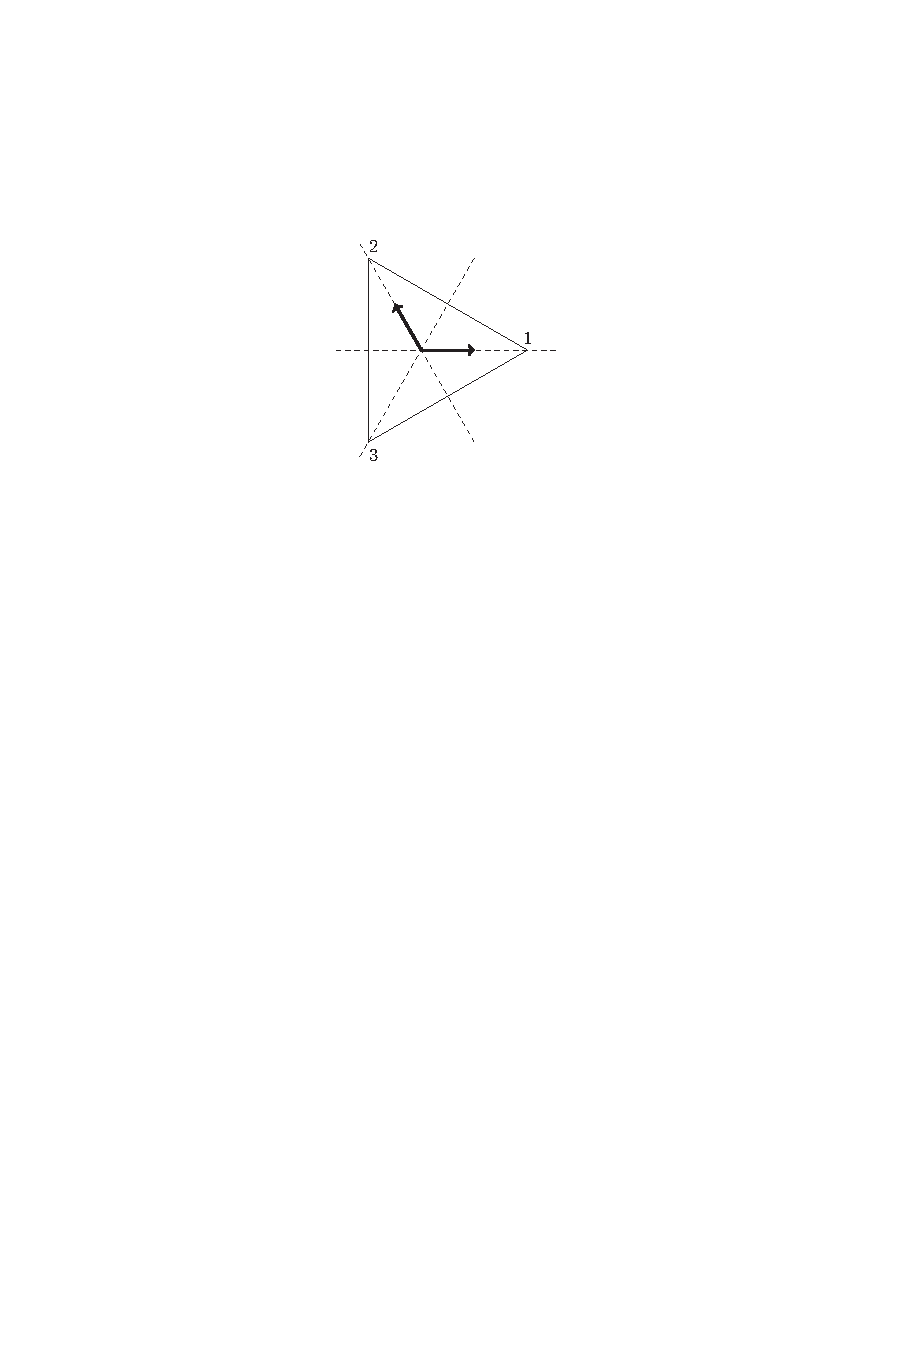
\includegraphics{pictures/rep-of-S_3-dim2}\]
Positioning the center of the triangle at the origin of $V$ and labeling the three vertices of the triangle as $1$, $2$, and $3$, we get a representation
\[\begin{array}{c}

(1,2)\mapsto\begin{pmatrix}
0&1\\
1&0
\end{pmatrix}\quad (23)\mapsto\begin{pmatrix}
-1&0\\
-1&1
\end{pmatrix}\quad (13)\mapsto\begin{pmatrix}
1&-1\\
0&-1
\end{pmatrix}\\
(123)\mapsto\begin{pmatrix}
0&-1\\
1&-1
\end{pmatrix}\quad(132)\mapsto\begin{pmatrix}
-1&1\\
-1&0
\end{pmatrix}
\end{array}\]
where we have taken basis vectors in the directions of vertices $1$ and $2$, making an angle of $2\pi/3$ to each other. In fact these matrices define a representation of degree $2$ over any ring $R$, because although the representation was initially constructed over $\R$ the matrices have integer entries, and these may be interpreted in every ring. No matter what the ring is, the matrices always multiply together to give a copy of $\mathfrak{S}_3$.
\end{example}
\begin{example}\label{representation C_p on F_p eg}
Let $R=\F_p$, $V=R^2$, and let $G=C_p=\langle g\rangle$ be cyclic of order $p$ generated by an element $g$. We see that the assignment
\[\rho(g^r)=\begin{pmatrix}
1&0\\
r&1
\end{pmatrix}\]
is a representation. In this case, the fact that we have a representation is very much dependent on the choice of $R$ as the field $\F_p$: in any other characteristic it would not work, because the matrix shown would no longer have order $p$.
\end{example}
We can think of representations in various ways. One of them is that a representation is the specification of an action of a group on an $R$-module, as we now explain. Given a representation $\rho:G\to GL(V)$, an element $v\in V$, and a group element $g\in G$, we get another module element $\rho(g)(v)$. Sometimes we write just $g\cdot v$ or $gv$ for this element. This rule for multiplication satisfies
\begin{align*}
g\cdot(av+bw)&=ag\cdot v+bg\cdot w,\\
(gh)\cdot v&=g\cdot(h\cdot v),\\
1\cdot v&=v
\end{align*}
for all $g\in G$, $v,w\in V$, and $a,b\in R$. A rule for multiplication $G\times V\to V$ satisfying these conditions is called a \textbf{linear action} of $G$ on $V$. To specify a linear action of $G$ on $V$ is the same thing as specifying a representation of $G$ on $V$, since given a representation, we obtain a linear action as indicated earlier, and evidently, given a linear action, we may recover the representation.\par
Another way to define a representation of a group is in terms of the group
algebra. We define the group algebra $R[G]$ (or $R[G]$) of $G$ over $R$ to be the free $R$-module with the elements of $G$ as an $R$-basis and with multiplication given on the basis elements by group multiplication. The elements of $R[G]$ are the (formal) $R$-linear combinations of group elements, and the multiplication of the basis elements is extended to arbitrary elements using bilinearity of the operation. What this means is that a typical element of $R[G]$ is an expression $\sum_{g\in G}a_gg$ where $a_g\in R$, and the multiplication of these elements is given symbolically by
\[\Big(\sum_{g\in G}a_gg\Big)\Big(\sum_{h\in G}b_hh\Big)=\sum_{k\in G}\Big(\sum_{gh=k}a_gb_h\Big)k.\]
Having defined the group algebra, we may now define a representation of $G$ over $R$ to be a $R[G]$-module. The fact that this definition coincides with the previous ones is the content of the next proposition. Throughout this text, we may refer to group representations as modules (for the group algebra).
\begin{proposition}
A representation of $G$ over $R$ has the structure of a $R[G]$-module. Conversely, every $R[G]$-module provides a representation of $G$ over $R$.
\end{proposition}
\begin{proof}
Given a representation $\rho:G\to\GL(V)$, we define a module action of $R[G]$ on $V$ by $(\sum a_gg)v=\sum a_g\rho(g)(v)$. Given an $R[G]$-module $V$, the linear map $\rho(g):v\mapsto g\cdot v$ is an automorphism of $V$ and $\rho(g_1)\rho(g_2)=\rho(g_1g_2)$ so $\rho:G\mapsto\GL(V)$ is a representation.
\end{proof}
The group algebra gives another example of a representation, called the \textbf{regular representation}. In fact, for any ring $A$, we may regard $A$ itself as a left $A$-module with the action of $A$ on itself given by multiplication of the elements. We denote this left $A$-module by $_{A}A$ when we wish to emphasize the module structure, and this is the (left) regular representation of $A$. When $A=R[G]$, we may describe the action on $R[G]$ by observing that each element $g\in G$ acts on $R[G]$ by permuting the basis elements in the fashion $g\cdot h=gh$. Thus, each $g$ acts by a permutation matrix. The regular representation is an example of a \textbf{permutation representation}, namely one in which every group element acts by a permutation matrix.\par
Regarding representations of $G$ as $R[G]$-modules has the advantage that many definitions we wish to make may be borrowed from module theory. Thus, we may study $R[G]$-submodules of an $R[G]$-module $V$, and if we wish, we may call them subrepresentations of the representation afforded by $V$. To specify an $R[G]$-submodule of $V$, it is necessary to specify an $R$-submodule $W$ of $V$ that is closed under the action of $R[G]$. This is equivalent to requiring that $\rho(g)w\in W$ for all $g\in G$ and $w\in W$. We say that a submodule $W$ satisfying this condition is \textbf{stable} under $G$ or that it is an \textbf{invariant submodule} or \textbf{invariant subspace} (if $R$ happens to be a field). Such an invariant submodule $W$ gives rise to a homomorphism $\rho_W:G\to\GL(W)$ that is the subrepresentation afforded by $W$.
\begin{example}\label{representation of C_2 semisimple}
Let $C_2=\{1,-1\}$ be cyclic of order $2$ and consider the representation
\[\rho:C_2\to\GL_2(\R),\quad 1\mapsto\begin{pmatrix}
1&0\\
0&1
\end{pmatrix},\quad -1\mapsto\begin{pmatrix}
1&0\\
0&-1
\end{pmatrix}\]
There are just four invariant subspaces, namely $\{0\}$, $\langle(\begin{smallmatrix}1\\0\end{smallmatrix})\rangle$, $\langle(\begin{smallmatrix}0\\1\end{smallmatrix})\rangle$, $\R^2$ and no others. The representation space $\R^2=\langle(\begin{smallmatrix}1\\0\end{smallmatrix})\rangle\oplus\langle(\begin{smallmatrix}0\\1\end{smallmatrix})\rangle$ is the direct sum of two invariant subspaces.
\end{example}
\begin{example}\label{representation of C_p on F_p non semisimple}
In Example~\ref{representation C_p on F_p eg}, an elementary calculation shows that $\langle(\begin{smallmatrix}0\\1\end{smallmatrix})\rangle$ is the only $1$-dimensional invariant subspace, and so it is not possible to write the representation space $V$ as the direct sum of two nonzero invariant subspaces.
\end{example}
We make use of the notions of a homomorphism and an isomorphism of $R[G]$-modules. Since $R[G]$ has as a basis the elements of $G$, to check that an $R$-linear homomorphism $f:V\to W$ is in fact a homomorphism of $R[G]$-modules, it suffices to check that $f(gv)=gf(v)$ for all $g\in G$---we do not need to check for every $x\in R[G]$. By means of the identification of $R[G]$-modules with representations of $G$ (in the first definition given here) we may refer to homomorphisms and isomorphisms of group representations.\par
If $V$ and $W$ are $R[G]$-modules then we may form their (external) direct sum
$V\oplus W$, which is the same as the direct sum of $V$ and $W$ as $R$-modules together with an action of $G$ given by $g(v,w)=(gv,gw)$. We also have the notion of the internal direct sum of $R[G]$-modules and write $U=V\oplus W$ to mean that $U$ has $R[G]$-submodules $V$ and $W$ satisfying $U=V+W$ and $V\cap W=0$. In this situation, we also say that $V$ and $W$ are direct summands of $U$.
\subsection{Semisimple representations}
We come now to our first nontrivial result, one that is fundamental to the study of representations over fields of characteristic zero, or characteristic not dividing the group order. This surprising result says that in this situation representations always break apart as direct sums of smaller representations. We do now require the ring $R$ to be a field, and in this situation, we will often use the symbols $F$ or $k$ instead of $R$.
\begin{theorem}[\textbf{Maschke}]
Let $V$ be a representation of the finite group $G$ over a field $k$ in which $|G|$ is invertible. Let $W$ be an invariant subspace of $V$. Then there exists an invariant subspace $W'$ of $V$ such that $V=W\oplus W'$ as
representations.
\end{theorem}
\begin{proof}
Let $\pi:V\to W$ be any projection of $V$ onto $W$ as vector spaces. Since $k$ is a field, we may always find such a projection by finding a vector space complement to $W$ in $V$ and projecting off the complementary factor. Then $V=W\oplus\ker(\pi)$ as vector spaces, but $\ker(\pi)$ is not necessarily invariant under $G$. Consider the map $\widetilde{\pi}:V\to V$ defined by
\[\widetilde{\pi}=\frac{1}{|G|}\sum_{g\in G}g\pi g^{-1}.\]
Then $\widetilde{\pi}$ is $k$-linear, and if $w\in W$ then
\begin{align*}
\widetilde{\pi}(w)=\frac{1}{|G|}\sum_{g\in G}g\pi(g^{-1} w)=\frac{1}{|G|}\sum_{g\in G}gg^{-1}w=w.
\end{align*}
Since furthermore $\widetilde{\pi}(v)\in W$ for all $v\in V$, $\widetilde{\pi}$ is a projection onto $W$ and so $V=W\oplus\ker(\widetilde{\pi})$. We show finally that $\ker(\widetilde{\pi})$ is an invariant subspace by verifying that $\widetilde{\pi}$ is an $kG$-module homomorphism: if $h\in G$ and $v\in V$ then
\begin{align*}
\widetilde{\pi}(hv)=\frac{1}{|G|}\sum_{g\in G}g\pi g^{-1}(hv)=h\frac{1}{|G|}\sum_{g\in G}h^{-1}g\pi g^{-1}h(v)=h\widetilde{\pi}(v).
\end{align*}
This finishes the proof.
\end{proof}
Because the next results apply more generally than to group representations,
we let $A$ be a ring and consider its modules. A nonzero $A$-module $V$ is
said to be \textbf{simple} or \textbf{irreducible} if $V$ has no $A$-submodules other than $0$ and $V$.
\begin{example}
When $A$ is an algebra over a field, every module of dimension $1$ is simple. In Example~\ref{representation of S_3 eg}, we have constructed three representations of $\R\mathfrak{S}_3$, and they are all simple. The trivial and sign representations are simple because they have dimension $1$, and the $2$-dimensional representation is simple because, visibly, no $1$-dimensional subspace is invariant under the group action. We will see later that this is a complete list of the simple representations of $\mathfrak{S}_3$ over $\R$.
\end{example}
\begin{proposition}\label{simple module is cyclic}
Let $S$ be a simple $A$-module, then there exists a maximal left ideal $I$ in $A$ such that $S\cong A/I$.
\end{proposition}
\begin{proof}
Let $x\in S$ be nonzero. Then the map $\varphi:a\mapsto ax$ is a nonzero homomorphism, and hence is surjective due the simplicity of $S$. This implies $S\cong A/I$ where $I=\ker\varphi$ is a left ideal. Moreover, if $I$ is not maximal, then $A/I$ contains a nontrivial left ideal, and hence is not simple. This is a contradiction.
\end{proof}
A module that is the direct sum of simple submodules is said to be \textbf{semisimple} or \textbf{completely reducible}. We saw in Examples~\ref{representation of C_2 semisimple} and \ref{representation of C_p on F_p non semisimple} two examples of modules, one of which was semisimple and the other of which was not.
\begin{lemma}\label{semisimple simple submodule}
If $M\neq 0$ and $M$ is semisimple, then it has a simple submodule.
\end{lemma}
\begin{proof}
Let $x\in M-\{0\}$, and set $M'=Ax$. Then $M'$ is semisimple and nonzero, so we may assume that $M=M'$.\par
Set
\[\mathcal{X}=\{\text{$N$ is a submodule of $M$ and $x\notin N$}\}.\]
This set is nonempty because it contains the zero submodule. If $\mathcal{Y}\sub \mathcal{X}$ is totally ordered, then $N=\bigcup_{N'\in \mathcal{Y}}N'$ is a submodule of $M$. Also, $x\notin N$ by definition of $N$, so $N$ is an element of $\mathcal{X}$, and an upper bound of $\mathcal{Y}$. By Zorn's lemma, $\mathcal{X}$ has a maximal element $N$.\par
As $x\notin N$, $N\neq M$. As $M$ is semisimple, there exists a submodule $N'$ of $M$ such that $M=N\oplus N'$, and we have $N'\neq 0$ because $N\neq M$. We claim that $N'$ is simple. Indeed, if there were a submodule $0\neq N''\sub N'$, then we would have $N\oplus N''\notin\mathcal{X}$ by maximality of $N$ in $X$, so $x\in N\oplus N''$, but then $N\oplus N''=M$ (because $M=Ax$), and hence $N''=N'$.
\end{proof}
\begin{theorem}\label{semisimple module iff}
Let $A$ be a ring and $M$ be a $A$-module. The following are equivalent:
\begin{itemize}
\item[(\rmnum{1})] $M$ is semisimple.
\item[(\rmnum{2})] $M$ is a direct sum of simple modules.
\item[(\rmnum{3})] $M$ is a sum of simple modules.
\end{itemize}
\end{theorem}
\begin{proof}
Assume that $M$ is semisimple. Let $M'$ be the sum of all the simple submodules of $M$, and choose a submodule $M''$ of $M$ such that $M=M'\oplus M''$. If $M''\neq 0$, then by the lemma $M''$ has a simple submodule $N$, but then we should have $N\sub M'$, which contradicts the fact that $M'$ and $M''$ are in direct sum. So $M'=M$. This proves $(\rmnum{1})\Rightarrow(\rmnum{2})$.\par
Now let $(M_i)_{i\in I}$ be the family of all simple submodules of $M$ and assume that $M=\sum_{i\in I}M_i$. Let $N$ be a submodule of $M$. We will show that there exists $J\sub I$ such that
\[M=N\oplus\bigoplus_{j\in J}M_j\]
This clearly implies $(\rmnum{1})$, and we also get $(\rmnum{2})$ by taking $N=0$.\par
To get $J$, we apply the Zorn's lemma. Set
\[\mathcal{X}=\{K\sub I\mid\text{$N+\sum_{k\in K}M_k$ is a direct sum}\}.\]
This set $\mathcal{X}$ is not empty, because $\emp\in\mathcal{X}$. Let $\mathcal{Y}\sub\mathcal{X}$ be a totally ordered subset and let $K=\bigcup\mathcal{Y}$. If there are $n\in N$ and $m_{i}\in\bigcup_{k\in K}M_{k},i=1,\dots,n$ such that $n+\sum_{i=1}^{n}m_{k_i}=0$, then since $\mathcal{Y}$ is totally ordered, there exists $L\in\mathcal{Y}$ such that $k_1,\dots,k_n\in\bigcup_{k\in L}M_k$. Since $L\in\mathcal{X}$, the fact $n+\sum_{i=1}^{n}m_{i}=0$ implies that $n=0$ and $m_i=0$ for every $i=1,\dots,n$. Therefore $N+\sum_{k\in K}M_k$ is a direct sum and $K\in\mathcal{X}$.\par
By Zorn's lemma, $\mathcal{X}$ has a maximal element $J$. Let $M'=N\oplus\bigoplus_{j\in J}M_j$. We will show that $M=M'$. Let $i\in I$, if $M_i\nsubseteq M'$, then $M'\cap M_i=0$ since $M_i$ is simple. But then
\[M'+M_i=N\oplus\bigoplus_{j\in J}M_j+M_i\]
is a direct sum. This means $J\cup\{i\}\in\mathcal{X}$, and contradicts the maximality of $J$.
\end{proof}
\begin{corollary}
Let $k$ be a field in which $|G|$ is invertible. Then every finite-dimensional $kG$-module is semisimple.
\end{corollary}
This result puts us in very good shape if we want to know about the representations of a finite group over a field in which $|G|$ is invertible---for example any field of characteristic zero. To obtain a description of all possible finite-dimensional representations, we need only describe the simple ones, and then arbitrary ones are direct sums of these.\par
\begin{proposition}
Let $A$ be a ring and $M$ be an $A$-module.
\begin{itemize}
\item[(a)] The sum of all the simple submodules of $M$ is a semisimple module, that is the unique largest semisimple submodule of $M$.
\item[(b)] The sum of all submodules of $M$ isomorphic to some given simple module $S$ is a submodule isomorphic to a direct sum of copies of $S$. It is the unique largest submodule of $S$ with this property.
\end{itemize}
\end{proposition}
\begin{proof}
For (a), the sum of all simple submodules of $M$ is semisimple by Theorem~\ref{semisimple module iff}, and since any semisimple submodule of $M$ is a sum of simple modules, this is clearly the largest one. A similar argument proves (b).
\end{proof}
The largest semisimple submodule of a module $M$ is called the \textbf{socle of $\bm{M}$}, and is denoted $\Soc(M)$. There is a dual construction called the \textbf{radical of $\bm{M}$}, denoted $\Rad(M)$, that we will study later. It is defined to be the intersection of all the maximal submodules of $M$, and has the property that it is the smallest submodule of $M$ with semisimple quotient.
\begin{proposition}\label{direct sum of simple module summand char}
Let $M=\bigoplus_{i=1}^{r}S_i^{n_i}$ be a semisimple module over a ring $A$, where the $S_i$ are nonisomorphic simple $A$-modules and the $n_i$ are their multiplicities as summands of $M$. Then each submodule $S_i^{n_i}$ is uniquely determined and is characterized as the unique largest submodule of $M$ expressible as a direct sum of copies of $S_i$.
\end{proposition}
\begin{proof}
It suffices to show that $S_i^{n_i}$ contains every submodule of $M$ isomorphic to $S_i$. If $N$ is any nonzero submodule of $M$ not contained in $S_i^{n_i}$, then for some $j\neq i$, its projection to a summand $S_j$ must be nonzero. If we assume that $N$ is simple, this projection will be an isomorphism $N\cong S_i$. Thus, all simple submodules isomorphic to $S_i$ are contained in the summand $S_i^{n_i}$.
\end{proof}
Now we give some nonsemisimple representations and compute their scoles.
\begin{example}
Let $K_4=\{1,x,y,xy\}$ be the Klein four-group, $R=\F_2$, and consider the representation $\rho_1$ on $V=(\F_2)^3$ specified on the generators of $G$ by
\[\rho_1(x)\cdot(a,b,c)=(a+b,b,c),\quad\rho_1(y)(a,b,c)=(a+c,b,c).\]
From these expressions, we immediately see that $V_1=\langle e_1\rangle$ is the unique invariant subspace of dimension $1$. Now assume that $W$ is an invariant subspace of dimension $2$. If $(a,b,c)\in W$ is an nonzero element, then we have
\[\rho_1(x)\cdot(a,b,c)-(a,b,c)=(b,0,0)\in V_1,\quad \rho_1(y)(a,b,c)-(a,b,c)=(c,0,0)\in V_1.\]
This implies any invariant subsapce of $\rho_1$ contains $V_1$, and so $V_1$ is the only irreducible subrepresentation of $\rho_1$. Therefore, the scole of $\rho_1$ is given by $V_1=\langle e_1\rangle$, with trivial action on it.\par
Now we consider another representation $\rho_2$ of $G$ on the same space given by
\[\rho_2(x)(a,b,c)=(a,b+c,c),\quad \rho_2(y)(a,b,c)=(a+c,b,c).\]
Therefore, it can be easily seen that $V_1=\langle e_1\rangle$ and $V_2=\langle(0,1,0)\rangle$ are both invariant subsapces of $\rho_2$. Note that if $(a,b,c)\in V$ with $c\neq 0$, then
\[\rho_2(x)(a,b,c)-(a,b,c)=(0,c,0)\in V_2,\quad\rho_2(y)(a,b,c)-(a,b,c)=(c,0,0)\in V_1.\]
This implies $V_1$ and $V_2$ are the only irreducible subrepresentation of $\rho_2$, and therefore the scole of $\rho_2$ is given by $V_1\oplus V_2$, with trivial action on it.
\end{example}
\begin{example}\label{representation of C_p on F_p}
Let $G=C_p=\langle x\rangle$ and $R=\F_p$ for some prime $p\geq 3$. Consider the two representations $\rho_1$ and $\rho_2$ specified by
\[\rho_1(x)=\begin{pmatrix}
1&1&0\\
0&1&1\\
0&0&1
\end{pmatrix}\quad\rho_2(x)=\begin{pmatrix}
1&1&1\\
0&1&0\\
0&0&1
\end{pmatrix}\]
and $V$ has a basis $\{e_1,e_2,e_3\}$. For $\rho_1$, it can be easily verified that $\langle e_1\rangle$ and $\langle e_1,e_2\rangle$ are invariant subspaces of $\rho_1$. Since $\langle e_1\rangle$ is the unique invariant subspace of one dimensional, it follows that the scole of $\rho_1$ is $\langle e_1\rangle$.\par
Similarly, it can be easily shown that $\langle e_1\rangle$ and $\langle e_2-e_3\rangle$ are invariant subspaces of $\rho_2$, and so the scole of $\rho_2$ is $\langle e_1\rangle\oplus\langle e_2-e_3\rangle$. Note that in this case we have a decomposition $V=\langle e_1,e_2\rangle\oplus\langle e_2-e_3\rangle$.
\end{example}
\begin{example}\label{representation of C_2 times C_2 char=2}
Let $k$ be an infinite field of characteristic $2$, and $G=\langle x,y\rangle\cong C_2\times C_2$ be the noncyclic group of order $4$. For each $\lambda\in k$, let $V_\lambda$ be a $k$-vector space of dimension $2$ with basis $\{e_1,e_2\}$, and $\rho_\lambda$ be the representation defined by
\[\rho_\lambda(x)=\begin{pmatrix}
1&0\\
1&1
\end{pmatrix}\quad\rho_\lambda(y)=\begin{pmatrix}
1&0\\
\lambda&1
\end{pmatrix}\]
Clearly $\langle e_1\rangle$ is the unique invariant subspace of $V_\lambda$, so the scole is given by $\Soc(V_\lambda)=\langle e_1\rangle$. By Schur lemma, if $\varphi:V_\lambda\to V_\mu$, we must have $\varphi(\Soc(V_\lambda))=\Soc(V_{\mu})$, and therefore $\varphi$ has the form
\[\varphi=\begin{pmatrix}
a&0\\
b&c
\end{pmatrix}\]
By a computation of the linear condition on $\varphi$, we get $\lambda=\mu$. Therefore $V_{\lambda}=V_{\mu}$ if and only if $\lambda=\mu$. This implies in particular that $kG$ has infinitely many nonisomorphic $2$-dimensional representations.
\end{example}
\subsection{Schur's lemma and Wedderburn's theorem}
Possibly the most important single technique in representation theory is to consider endomorphism rings. It is the main technique of this part, and we will see it in use throughout this chapter. The first result is basic and will be used time and time again.
\begin{theorem}[\textbf{Schur's lemma}]
Let $A$ be a ring and let $M$ and $N$ be $A$-modules, and $\varphi:M\to N$ be a $A$-linear map.
\begin{itemize}
\item If $M$ is simple, then $\varphi=0$ or $\varphi$ is injective.
\item If $N$ is simple, then $\varphi=0$ or $\varphi$ is surjective.
\item If $M$ and $N$ are simple, then $\varphi=0$ or $\varphi$ is an isomorphism.
\end{itemize}
In particular, if $M$ is a simple $A$-module, then $\End_A(M)$ is a division ring.
\end{theorem}
\begin{proof}
Since $\ker\varphi$ and $\im\varphi$ are both submodules, these claims follow from the definition of simplicity.
\end{proof}
\begin{corollary}\label{endomorphism of simple module scalar}
Let $A$ be a finite-dimensional algebra over an algebraically closed field $k$, and $S$ be a simple $A$-module. Then every endomorphism in $\End_A(S)$ is multiplication by some scalar. Thus, $\End_A(S)\cong k$ in this case.
\end{corollary}
\begin{proof}
If $A$ is a finite-dimensional $k$-algebra and $k$ is algebraically closed then $S$ is a finite-dimensional vector space by Proposition~\ref{simple module is cyclic}. Let $\varphi$ be an $A$-module endomorphism of $S$ and let $\lambda$ be an eigenvalue of $\varphi$. Now $(\varphi-\lambda I):S\to S$ is a singular endomorphism of $A$-modules, so $\varphi-\lambda I=0$ and $\varphi=\lambda I$.
\end{proof}
We have seen in Maschke's theorem that if $k$ is a field and $|G|$ is invertible then every $kG$-module is semisimple. We now consider the exact condition under which all modules are semisimple. It has the following description.
\begin{theorem}\label{semisimple ring iff}
Let $A$ be a ring. The following are equivalent:
\begin{itemize}
\item[(\rmnum{1})] All short exact sequences of $A$-modules split.
\item[(\rmnum{2})] All $A$-modules are semisimple.
\item[(\rmnum{3})] All finitely generated $A$-modules are semisimple.
\item[(\rmnum{4})] All cyclic $A$-modules are semisimple.
\item[(\rmnum{5})] The left regular $A$-module $_{A}A$ is semisimple.
\end{itemize}
If these conditions are satisfied, then we say that the ring $A$ is \textbf{semisimple}.
\end{theorem}
A priori, this notion should be called \textbf{left semisimple ring}, and we should have a similarly defined notion of \textbf{right semisimple ring}. But we will see that left semisimple and right semisimple are actually equivalent, so we just use the name semisimple ring.
\begin{proof}
The condition $(\rmnum{1})$ is easily seen to be equivalent to $(\rmnum{2})$ from the definition of semisimple modules, and the implications $(\rmnum{2})\Rightarrow(\rmnum{3})\Rightarrow(\rmnum{4})\Rightarrow(\rmnum{5})$ are obvious. Now we prove $(\rmnum{5})\Rightarrow(\rmnum{2})$. Let $M$ be a $A$-module. If $x\in M$, then $Ax\sub M$ is a quotient of $_{A}A$, so it's semisimple because $_{A}A$ is semisimple. As $M=\sum_{x\in M}Ax$, Theorem~\ref{semisimple module iff} implies that $M$ is semisimple.
\end{proof}
The next result is the main tool in recovering the structure of an algebra from its representations, which will be used in our structural theorem of semisimple rings. We use the notation $A^{op}$ to denote the opposite ring of $A$, namely, the ring that has the same set and the same addition as $A$, but with a reverse multiplication.
\begin{lemma}\label{endomorphism of _AA is right multiplication}
For any ring $A$ we have $\End_A(_{A}A)\cong A^{op}$.
\end{lemma}
\begin{proof}
We prove the result by writing down homomorphisms in both directions
that are inverse to each other. The inverse isomorphisms are
\begin{align*}
&\Phi:\End_A(_{A}A)\to A^{op},\quad \phi\mapsto\phi(1),\\
&\Psi:A^{op}\to\End_A(_{A}A),\quad x\mapsto(a\mapsto ax).
\end{align*}
Note that the map $a\mapsto ax$ takes value in $\End_{A}(_{A}A)$ because $_{A}A$ is a left module. Now we check that these are homomorphisms of rings. To distinguish, we denote the multiplication in $A^{op}$ by $a\ast b$, and the multiplication in $A$ be $a\cdot b$. We compute that
\begin{align*}
&\Phi(\phi\circ\psi)=\phi\circ\psi(1)=\phi(\psi(1))=\phi(\psi(1)\cdot 1)=\psi(1)\phi(1)=\phi(1)\ast\psi(1),\\
&\Phi(\phi+\psi)=(\phi+\psi)(1)=\phi(1)+\psi(1),\\
&\Phi(\id)=\id(1)=1,
\end{align*}
and
\begin{align*}
&\Psi(x\ast y)(a)=a(x\ast y)=ayx=(ay)x=\Psi(x)(ay)=\Psi(x)\circ\Psi(y)(a),\\
&\Psi(x+y)(a)=a(x+y)=ax+ay=\Psi(x)(a)+\Psi(y)(a),\\
&\Psi(1)(a)=a=\id(a).
\end{align*}
Therefore $\Phi$ and $\Psi$ are both homomorphism of rings. Finally, for $\phi\in\End_{A}(_{A}A)$ and $x\in A^{op}$, we observe that
\[\Psi(\Phi(\phi))(a)=\Psi(\phi(1))(a)=a\phi(1)=\phi(a),\quad \Phi(\Psi(x))=\Psi(x)(1)=x,\]
which imply that $\Phi\circ\Psi=\Psi\circ\Phi=\id$, completing the proof.
\end{proof}
\begin{remark}
Observe that the proof of Lemma~\ref{endomorphism of _AA is right multiplication} establishes that every endomorphism of the regular representation is a right multiplication.
\end{remark}
\begin{theorem}[\textbf{Artin-Wedderburn}]\label{Artin-Wedderburn}
Let $A$ be a finite-dimensional algebra over a field $k$ with the property that every finite-dimensional module is semisimple. Then $A$ is a direct sum of matrix algebras over division rings. Specifically, if
\[_{A}A\cong S_1^{n_1}\oplus\cdots\oplus S_r^{n_r}\]
where the $S_1,\dots,S_r$ are nonisomorphic simple modules occuring with multiplicities $n_1,\dots,n_r$ in the regular representation, then
\[A\cong\mathcal{M}_{n_1}(D_1)\times\cdots\times\mathcal{M}_{n_r}(D_r)\]
where $D_i=\End_A(S_i)^{op}$. Furthermore, if $k$ is algebraically closed then $D_i=k$ for all $i$.
\end{theorem}
\begin{proof}
We first observe that if we have a direct sum decomposition
\[M=M_1\oplus\cdots\oplus M_r\]
of a module $M$ then $\End_A(M)$ is isomorphic to the algebra of $r\times r$ matrices in which the $(i,j)$ entries lie in $\Hom_A(M_j,M_i)$. This is because any endomorphism $\phi:M\to M$ may be writen as a matrix of components $\phi=(\phi_{i,j})$ where $\phi_{i,j}:M_j\to M_i$, and when viewed in this way endomorphisms compose in the manner of matrix multiplication. Since $\Hom_A(S_j^{n_j},S_i^{n_i})=0$ if $i\neq j$ by Schur's Lemma, the decomposition of $_{A}A$ shows that
\[\End_A(_{A}A)\cong \End_A(S_1^{n_1})\times\cdots\times\End_A(S_r^{n_r})\cong\mathcal{M}(\End_A(S_1))\times\cdots\times\mathcal{M}(\End_A(S_i)).\]
Furthermore, consider the map
\[\Phi:\mathcal{M}_{n_i}(\End_A(S_i))^{op}\to\mathcal{M}_{n_i}(\End_A(S_i)^{op}),\quad A\mapsto A^T.\]
It is clear that $\Phi$ is bijective; it is a homomorphism since
\begin{align*}
\Phi(A\ast B)_{ij}=\Phi(BA)_{ij}=(BA)^T_{ij}=(A^TB^T)_{ij}=(\Phi(A)\Phi(B))_{ij}.
\end{align*}
Therefore we see that $\mathcal{M}_{n_i}(\End_A(S_i))^{op}\cong\mathcal{M}_{n_i}(\End_A(S_i)^{op})=\mathcal{M}_{n_i}(D_i)$. Since we can identify $\End_A(_{A}A)$ as $A^{op}$, putting these pieces together gives the matrix algebra decomposition. Finally, if $k$ is algebraically closed, it follows from Schur's Lemma that $D_i=k$ for all $i$.
\end{proof}
We now determine the multiplicities appear in the decomposition of Theorem~\ref{Artin-Wedderburn}.
\begin{proposition}\label{Artin-Wedderburn multiplicity}
Let $A$ be a finite-dimensional semisimple $k$-algebra, $S$ a simple $A$-module and $D=\End_A(S)$. Then $S$ may be regarded as a module over $D$ and the multiplicity of $S$ as a summand of $_{A}A$ equals $\dim_DS$. In particular, if $k$ is algebraically closed then the multiplicity of $S$ equals $\dim_k S$.
\end{proposition}
\begin{proof}
If $M$ is any finite-dimensional $A$-module and $M\cong\bigoplus_iS_i^{n_i}$ is a decomposition into pairwise non-isomorphic simple $A$-modules $S_i$ then
\begin{align*}
\Hom_A(M,S)&=\Hom_A(\bigoplus_iS_i^{n_i},S)=\prod_{i}\Hom_A(S_i^{n_i},S)\\
&=\Hom_A(S^n,S)=\Hom_A(S,S)^n=\End_A(S)^n=D^n,
\end{align*}
as $k$-vector spaces, where $n$ is the multiplicity of $S$ in $M$. It follows that
\[\dim_k\Hom_A(M,S)=n\dim_kD,\]
and therefore
\[n=\frac{\dim_k\Hom_A(M,S)}{\dim_kD}=\dim_{D}\Hom_A(M,S).\]
Take $M=A$, since $\Hom_A(A,S)\cong S$ as $k$-vector spaces, we conclude the claim.
\end{proof}
\begin{corollary}\label{semisimple ring decomposition multiplicity}
Let $A$ be a finite-dimensional semisimple algebra over a field $k$. In any decomposition,
\[_{A}A=S_1^{n_1}\oplus\cdots\oplus S_r^{n_r}\]
where the $S_i$ are pairwise nonisomorphic simple modules, we have that $S_1,\dots,S_r$ is a complete set of representatives of the isomorphism classes of simple $A$-modules. If $k$ is algebraically closed, then $n_i=\dim_kS_i$ and $\dim_k A=n_1^2+\cdots+n_r^2$.
\end{corollary}
\begin{proof}
All isomorphism types of simple modules must appear in the decomposition because every simple module can be expressed as a homomorphic image of $_{A}A$, and so must be a homomorphic image of one of the modules $S_i$. When $k$ is algebraically closed all the division rings $D_i$ coincide with $k$ by Schur's Lemma, and $\End_A(S_i^{n_i})\cong\mathcal{M}_{n_i}(k)$. The ring decomposition $A=\mathcal{M}_{n_1}(k)\times\cdots\times\mathcal{M}_{n_r}(k)$ of Theorem~\ref{Artin-Wedderburn} immediately gives $\dim_kA=n_1^2+\cdots+n_r^2$ and $\dim_kS_i=n_i$.
\end{proof}
Let us now restate what we have proved specifically in the context of group representations.
\begin{corollary}
Let $G$ be a finite group and $k$ a field in which $|G|$ is invertible. Then as a ring, $kG$ is a direct sum of matrix algebras over division rings.
\end{corollary}
\begin{corollary}\label{representation degree sum formula}
Let $G$ be a finite group and $k$ a algebraically closed in which $|G|$ is invertible. Let $S_1,\dots,S_r$ be a complete set of representatives of the simple $kG$-modules, with $d_i=\dim_kS_i$. Then $d_i$ is the multiplicity with which $S_i$ is a summand of the regular representation of $G$, and
\[|G|=\sum_{i=1}^{r}d_i^2.\]
\end{corollary}
\begin{proof}
This follows from Maschke's theorem, the Artin-Wedderburn theorem, and Corollary~\ref{semisimple ring decomposition multiplicity}.
\end{proof}
The result above provides a numerical criterion that enables us to say when we have constructed all the simple modules of a group over an algebraically closed field $k$ in which $|G|$ is invertible: we check that $\sum_id_i^2=|G|$. While this is an easy condition to verify, it will be superseded later on by the even more straightforward criterion that the number of simple $kG$-modules (with the same hypotheses on $k$) equals the number of conjugacy classes of elements of $G$. Once we have proved this, the formula $\sum_id_i^2=|G|$ allows the degree of the last simple representation to be determined once the others are known.
\begin{example}
In Example~\ref{representation of S_3 eg}, we have seen three representations of $\mathfrak{S}_3$ over $\R$ that are simple: the trivial representation, the sign representation, and a $2$-dimensional representation. Since $1^2+1^2+2^2=|\mathfrak{S}_3|$, we have constructed
all the simple representations of $\mathfrak{S}_3$ over $\R$.
\end{example}
At this point, we make a deduction about representations of finite abelian
groups.
\begin{corollary}\label{representation of finite abelian group}
Let $G$ be a finite abelian group. Over an algebraically closed field $k$ in which $|G|$ is invertible, every simple representation of $G$ has degree one and the number of nonisomorphic simple representations equals $|G|$.
\end{corollary}
\begin{proof}
We know that $kG$ is semisimple, and because $kG$ is a commutative ring the matrix summands that appear in Theorem~\ref{Artin-Wedderburn} must all have size $1$, and the division rings that appear must be commutative. In fact, since we have supposed that $k$ is algebraically closed, the division rings must all be $k$. This means that the degrees of the irreducible representations are all $1$, and so the number of them must be $|G|$ since this is the sum of the degrees.
\end{proof}
\begin{example}
Let $A$ be a finite-dimensional semisimple algebra. Then since $A$ has only finitely many simple modules, the isomorphism types of $A$-modules in each dimension is finite. Note that this is not in general true for algebras that are not semisimple: in Example~\ref{representation of C_2 times C_2 char=2} we saw that $k[C_2\times C_2]$ has infinitely many nonisomorphic $2$-dimensional representations when $k$ is an infinite field of characteristic $2$.
\end{example}
\begin{example}
Let $T$ be an invertible matrix of finite order, with order relatively prime to the characteristic of $k$. Then $T$ gives a representation of the cyclic group it generates on the space of vectors on which the matrix acts. Moreover, by invertibility of the order, the representation is semisimple. It is a direct sum of $1$-dimensional spaces by Corollary~\ref{representation of finite abelian group}. On choosing basis vectors to lie in these $1$-dimensional spaces, the matrix is diagonal.
\end{example}
\begin{example}\label{representation cyclic group eg}
Let $G=\langle g\rangle$ be a cyclic group of order $n$ and $k$ a field. By considering the homomorphism $k[x]\to kG$ which sends $x$ to $g$, we see that $kG\cong k[x]/(x^n-1)$ as rings. Let $x^n-1=p_1(x)^{d_1}\cdots p_r(x)^{d_r}$ be the factorization of $x^n-1$ in $k[x]$, where $p_i(x)$ are irreducible and coprime, then by the Chinese remainder theorem,
\[kG\cong\frac{k[x]}{(x^n-1)}\cong\frac{k[x]}{(p_1(x)^{n_1})}\times\cdots\times\frac{k[x]}{(p_r(x)^{n_r})}.\]
Since every simple $A$-module is the quotient of $A$ by a maximal ideal (Proposition~\ref{simple module is cyclic}), it follows that every simple module in $k[x]/(x^n-1)$ is isomorphism to $k[x]/(p(x))$, for some irreducible factor $p(x)$ of $x^n-1$.\par
Suppose that the characteristic of $k$ does not divide $n$. Then since $x^n-1$ is separable, $d_i=1$ for all $i$. Therefore each ideal $(p_i(x))$ is maximal, and it follows that
\[kG\cong\frac{k[x]}{(p_1(x))}\times\cdots\times\frac{k[x]}{(p_r(x))}\]
is the decomposition of $kG$. Let $S_i$ be the simple module corresponding to $p_i(x)$, then $\dim_kS_i=\deg p_i(x)$. Since $n=\sum_{i=1}^{r}\deg p_i(x)$, it follows that each component $S_i$ appears in $kG$ exactly once. Therefore, in view of Proposition~\ref{Artin-Wedderburn multiplicity}, we conclude that $\End_{kG}(S_i)\cong k[x]/(p_i(x))$.\par
In particular, if $k$ is algebraically closed, then all irreducible representations of $G$ have degree $1$.\par
Let $n$ be a prime and $k=\Q$, so that $x^n-1/(x-1)=x^{n-1}+x^{n-2}+\cdots+1$ is irreducible. By the preceeding arguments, there is a simple module $S$ such that $\End_{kG}(S)\cong\Q(e^{2\pi i/n})$.\par
Finally, consider $k=\R$. In this case we have the following factorizations of $x^n-1$:
\begin{align*}
&x^{2n}-1=\prod_{k=1}^{n}(x-e^{\frac{2\pi ki}{2n}})(x-e^{-\frac{2\pi ki}{2n}})=(x+1)(x-1)\prod_{i=1}^{n-1}(x^2-2\cos\frac{k\pi}{n}x+1),\\
&x^{2n+1}-1=(x-1)\prod_{k=1}^{n}(x-e^{\frac{2\pi ik}{2n+1}})(x-e^{-\frac{2\pi ik}{2n+1}})=(x-1)\prod_{i=1}^{n}(x^2-2\cos\frac{2k\pi}{2n+1}x+1).
\end{align*}
Therefore, when $n$ is odd, $G$ has $(n-1)/2$ simple representations of degree $2$ as well as the trivial representation of degree $1$; when $n$ is even, $G$ has $(n-2)/2$ simple representations of degree $2$ as well as two simple representations of degree $1$. If $S$ is one of the simple representations of degree $2$, then $\End_{\R G}(S)\cong\C$.
\end{example}
\begin{example}\label{representation of Q_8 is H}
Let $\H$ be the algebra of quaternions, that has a basis over $\R$ consisting of elements $\mathbf{1}$, $\mathbf{i}$, $\mathbf{j}$, $\mathbf{k}$ and multiplication determined by the relations
\[\mathbf{i}^2=\mathbf{j}^2=\mathbf{k}^2=\mathbf{ijk}=-1.\]
The elements $\{\pm 1,\pm\mathbf{i},\pm\mathbf{j},\pm\mathbf{k}\}$ 0form the quaternion group $Q_8$ of order $8$, and it acts on $\H$ by left multiplication, so that $\H$ is a $4$-dimensional representation of $Q_8$ over $\R$.
\end{example}
\section{Characters}
\subsection{The character table}
Assume that $\rho:G\to\GL(V)$ is a finite-dimensional representation of $G$ over the field of complex numbers $\C$ or one of its subfields. We define the \textbf{character} $\chi$ of $\rho$ to be the function $\chi:G\to\C$ given by
\[\chi(g)=\tr(\rho(g))\]
the trace of the linear map $\rho(g)$. The degree of the character is $\dim V$, which equals $\chi(1)$. We say that the representation $\rho$ and the representation space $V$ afford the character $\chi$, and we may write $\chi_{\rho}$ or $\chi_{V}$ when we wish to specify this character more precisely. The restriction to subfields of $\C$ is not significant: we will see in future that representations of a finite group over a field characteristic $0$ may always be realized over $\C$.\par
We now list some immediate properties of characters.
\begin{proposition}\label{character prop}
Let $\chi$ be the character of a representation $\rho$ of $G$ over $\C$ and let $g,h\in G$. Then
\begin{itemize}
\item[(a)] $\chi(1)$ is the degree of $\rho$, namely, the dimension of the representation space of $\rho$;
\item[(b)] if $g$ has order $n$ then $\chi(g)$ is a sum of $n$-th roots of unity;
\item[(c)] $|\chi(g)|\leq\chi(1)$, with equality if and only if $\rho(g)$ is scalar multiplication;
\item[(d)] $\chi(g)=\chi(1)$ if and only if $\rho(g)=1$, that is, $g$ lies in the kernel of $\rho$;
\item[(e)] $\chi(g^{-1})=\widebar{\chi(g)}$, the complex conjugate;
\item[(f)] $\chi(hgh^{-1})=\chi(g)$;
\item[(g)] if $V$ and $W$ are isomorphic $\C[G]$-modules then $\chi_V=\chi_W$ as functions on $G$.
\end{itemize}
\end{proposition}
\begin{proof}
Part (a) is immediate because the identity of the group must act as the identity matrix, and its trace is the degree of $\rho$, since this is the dimension of the representation space of $\rho$. For (b), recall that $\rho(g)$ is diagonalizable, so that $\chi(g)$ is the sum of its eigenvalues $\lambda_1,\dots,\lambda_d$, where $d$ is the degree of $\chi$. These eigenvalues are $n$-th roots of unity since $g$ has finite order $n$. From this we get the inequality $|\chi(g)|\leq|\lambda_1|+\cdots+|\lambda_d|=d$, and the equality holds if and only if $\lambda_1=\cdots=\lambda_d$ so that $\rho(g)$ is scalar. This proves (c).\par
For (d), if $\rho(g)=1$ then clearly $\chi(g)=\chi(1)$. Conversely, if $\chi(g)=d$ then by part (c), $\rho(g)$ is multiplication by a scalar $\lambda$. Now $\chi(g)=d\lambda=d$, so $\lambda=1$.\par
If $\lambda_1,\dots,\lambda_d$ are the eigenvalues of $\rho(g)$, then $\lambda_1^{-1},\dots,\lambda_d^{-1}$ are those of $\rho(g^{-1})$. Since $\lambda_i$ are roots of unity, we have $\lambda_i^{-1}=\widebar{\lambda_i}$. This gives (e).\par
Part (f) just a fact that $\tr(AB)=\tr(BA)$. For (g), suppose that $\rho_V$ and $\rho_W$ are the representations of $G$ on $V$ and $W$, and that we have an isomorphism of $\C[G]$-modules $\alpha:V\to W$. Then $\alpha\rho_V(g)=\rho_W(g)\alpha$ for all $g\in G$, so that
\[\chi_W(g)=\tr(\rho_W(g))=\tr(\alpha\rho_V(g)\alpha^{-1})=\tr(\rho_V(g))=\chi_V(g).\]
This finishes the proof.
\end{proof}
As an application of Proposition~\ref{character prop}(d), we see that certain normal subgroups, namely, the kernels of representations, are determined by knowing the characters of the representations. We will see that all normal subgroups of a finite group may be found from knowledge of the characters of representations, as intersections of the kernels of simple characters. This means that whether or not a group is simple may be easily read from this information on characters.\par
We see in Proposition~\ref{character prop}(f) that characters are constant on conjugacy classes, so that in listing values of characters on group elements we only need take one element from each conjugacy class. The table of complex numbers whose rows are indexed by the isomorphism types of simple representations of $G$, whose columns are indexed by the conjugacy classes of $G$ and whose entries are the values of the characters of the simple representations on representatives of the conjugacy classes is called the \textbf{character table} of $G$. It is usual to index the first column of a character table by the (conjugacy class of the) identity, and to put the character of the trivial representation as the top row. With this convention the top row of every character table will be a row of $1$'s, and the first column will list the degrees of the simple representations. Above the table, it is usual to list two rows, the first of which is a list of cardinalities of each conjugacy classes of $G$, in some notation. The row underneath lists a representative for each conjugacy in the top row.
\begin{example}
We present the character table of $\mathfrak{S}_3$. We sawthat we already have a complete list of the simple modules for $\mathfrak{S}_3$, and the values of their characters on representatives of the conjugacy classes of $\mathfrak{S}_3$ are computed from the matrices that give these representations.
\begin{table}[h]
\centering
\begin{tabular}{c|ccc}
\toprule
$\mathfrak{S}_3$&$1$&$3$&$2$\\
$g$&$1$&$(12)$&$(123)$\\
\midrule
$\chi_1$&$1$&$1$&$1$\\
$\chi_{\sgn}$&$1$&$-1$&$1$\\
$\chi_2$&$2$&$0$&$-1$\\
\bottomrule
\end{tabular}
\caption{Character table of $\mathfrak{S}_3$.}
\end{table}
\end{example}
\begin{example}
We consider the representation of $(\Z/2\Z)^n$. First, note that
\[\rho_1:[1]\mapsto 1,\quad \rho_2:[1]\mapsto-1\]
are all irreducible representations of $\Z/2\Z$. For each $Y\sub\{1,2,\dots,n\}$, we define a representation of $(\Z/2\Z)^n$ by
\[\rho_Y(g_1,g_2,\dots,g_n)=\prod_{i=1}^{n}\rho_{\iota_i}(g_i)\]
where $\iota_i=2$ for $i\in Y$. We can compute that for $n=(g_1,\cdots,g_n)$,
\[\chi_Y(g)=\prod_{i=1}^{n}\chi_{\iota_i}(g_i)=(-1)^{|\alpha(g)\cap Y|}.\]
Each $\rho_Y$ is a degree one representation, hence is irreducible. Since there are $2^n$ such representations, by Proposition~\ref{representation of finite abelian group} these are all irreducible representaions of $(\Z/2\Z)^n$.
\end{example}
We will see that the character table has remarkable properties, among which
are that it is always square, and its rows (and also its columns) satisfy certain orthogonality relations. Our next main goal is to state and prove these results. To do this, we first introduce three ways to construct new representations of a group from existing ones. These constructions have validity no matter what ring $R$ we work over, although in the application to the character table we will suppose that $R=\C$.\par
Suppose $V$ and $W$ are representations of $G$ over $R$. The $R$-module $V\otimes_RW$ acquires an action of $G$ by means of the formula $g\cdot(v\otimes w)=gv\otimes gw$, thereby making the tensor product into a representation. This is what is called the \textbf{tensor product} of the representations $V$ and $W$, but it is not the only occurrence of tensor products in representation theory, and as the other ones are different this one is sometimes also called the \textbf{Kronecker product}. The action of $G$ on the Kronecker product is called the \textbf{diagonal action}. To do things properly, we should check that the formula for the diagonal action does indeed define a representation of $G$. This is immediate, but the fact that we can make the definition at all is special for finite groups and group algebras: it does not work for algebras in general.\par
For the second construction, we form the $R$-module $\Hom_R(V,W)$. This acquires an action of $G$ by means of the formula $(g\cdot f)(v)=gf(g^{-1}v)$ for each $R$-linear map $f:V\to W$ and $g\in G$. It is worth checking that the negative exponent in the formula is really necessary so that we have a left action of $G$. Thus, $\Hom_R(V,W)$ becomes an $R[G]$-module.\par
The third construction is the particular case of the second in which we take $W$ to be the trivial module $R$. We write $V^*=\Hom_R(V,R)$ and the action is $(g\cdot f)(v)=f(g^{-1}v)$ for each $f:V\to R$ and $g\in G$. This representation is called the dual or contragredient representation of $V$. It is usually only considered when $V$ is free (or at least projective) of finite rank as an $R$-module, in which case we have $V\cong V^{**}$ as $R[G]$-modules. The exponent $-1$ in the action of $G$ is necessary to make $V^*$ a left $R[G]$-module. Without this exponent we would get a right $R[G]$-module.\par
If $R$ happens to be a field and we have bases $v_1,\dots,v_m$ for $V$ and $w_1,\dots,w_n$ for $W$ then $V\otimes W$ has a basis $\{v_i\otimes w_j:1\leq i\leq m,1\leq j\leq n\}$ and $V^*$ has a dual basis $v^1,\dots,v^m$. With respect to these bases an element $g\in G$ acts on $V\otimes W$ with the matrix that is the tensor product of the two matrices giving its action on $V$ and $W$, and on $V^*$ it acts with the transpose of the inverse of the matrix of its action on $V$. If $\alpha:V\to W$ and $\beta:W\to W$ are endomorphisms, then the matrix of
\[\alpha\otimes\beta:V\otimes W\to V\otimes W\]
is the tensor product of the matrices that represent $\alpha$ and $\beta$. We see from this that $\tr(\alpha\otimes\beta)=\tr(\alpha)\tr(\beta)$.\par
In the following result, we consider the sum and product of characters, which are defined in the usual manner for functions by the formulas
\[(\chi_V+\chi_W)(g)=\chi_V(g)+\chi_W(g),\quad(\chi_V\cdot\chi_W)(g)=\chi_V(g)\chi_W(g)\]
\begin{proposition}\label{character of sum and tensor prod}
Let $V$ and $W$ be finite-dimensional representations of $G$ over a field $k$ of characteristic zero.
\begin{itemize}
\item[(a)] $V\oplus W$ has character $\chi_V+\chi_W$.
\item[(b)] $V\otimes W$ has character $\chi_V\cdot\chi_W$.
\item[(c)] $V^*$ has character $\chi_{V^*}(g)=\chi_V(g^{-1})=\widebar{\chi_V(g)}$, the complex conjugate.
\item[(d)] Let $V$ and $W$ be representations of $G$ over any ground ring $R$. Suppose that, as an $R$-module, at least one of $V$ and $W$ is free of finite rank, then $\Hom_R(V,W)\cong V^*\otimes_RW$ as $R[G]$-modules. When $R=k$ is a field of characteristic zero this representation has character equal to $\chi_{V^*}\chi_W$.
\end{itemize}
\end{proposition}
\begin{proof}
Part (a), (b), and (c) are immediate from Proposition~\ref{character prop} and the subsequent remarks. For (d), we define an R-module homomorphism
\[\alpha:V^*\otimes W\to\Hom_R(V,W),\quad \phi\otimes v\mapsto(u\mapsto\phi(u)\cdot v).\]
this being the specification on basic tensors. We show that if either $V$ or $W$ is free as an $R$-module of finite rank then $\alpha$ is an isomorphism.\par
Suppose that $V$ is free, with basis $v_1,\dots,v_m$. Then $V^*$ is free with basis $v^1,\dots,v^m$ where $v^i(v_j)=\delta_{i,j}$. Any morphism $f:V\to W$ is determined by its values $f(v_i)$ on the basis elements by means of the formula $f(v)=\sum_{i=1}^{m}v^i(v)f(v_i)$ and it follows that $f=\alpha(\sum_{i=1}^{m}v^i\otimes f(v_i))$ so that $\alpha$ is surjective. If $\alpha(\sum_{i=1}^{m}v^i\otimes w_i)=0$ for certain elements $w_i\in N$ then applying this map to $v_j$ gives $w_j$, so we deduce $w_j=0$ for all $j$, and hence $\sum_{i=1}^{m}v^i\otimes w_i=0$. Thus, $\alpha$ is injective.\par
If $W$ is free as an $R$-module with basis $w_1,\dots,w_n$, let $p_i:W\to R$ be projection onto coordinate $i$. Any morphism $f:V\to W$ equals $\alpha(\sum_{i=1}^{n}p_if\otimes w_i)$, so $\alpha$ is surjective. If $\alpha(\sum_{i=1}^{n}\phi_i\otimes w_i)=0$ for certain $\phi_i\in V^*$ then for any $v\in V$, $\sum_{i=1}^{n}\phi_i(v)w_i=0$, which implies that $\phi_i(v)=0$ for all $i$ and $v$. This means that $\phi_i$ is the zero map for all $i$, so that $\sum_{i=1}^{n}\phi_i\otimes w_i=0$ and $\alpha$ is injective.\par
We now observe that $\alpha$ is a map of $R[G]$-modules, since for $g\in G$,
\begin{align*}
\alpha(g(\phi\otimes w))&=\alpha(g\phi\otimes gw)=(v\mapsto(g\phi)(v)\cdot gw)\\
&=(v\mapsto g(\phi(g^{-1}v)w))=g(v\mapsto\phi(v)w)\\
&=g\alpha(\phi\otimes w).
\end{align*}
Finally, the last formula for characters follows from parts (b) and (c).
\end{proof}
Of course, if $R$ is taken to be a field in part (d) of Proposition~\ref{character of sum and tensor prod} then the argument can be simplified. Since $V$ and $W$ are always free as $R$-modules in this situation, only one of the two arguments given is needed. After showing that $\alpha$ is either surjective or injective, the other follows by observing that the dimensions on the two sides are equal.
\subsection{Orthogonality relations and bilinear forms}
We start with some preliminary constructions that will be used in the proof of the orthogonality relations for characters. A fundamental notion in dealing with group actions is that of fixed points. If $V$ is an $R[G]$-module, we define the fixed points
\[V^G=\{v\in V:g\cdot v=v\text{ for all }g\in G\}.\]
This is the largest $R[G]$-submodule of $V$ on which $G$ has trivial action.
\begin{lemma}\label{representation fix point of Hom}
Over any ring $R$, $\Hom_R(V,W)^G=\Hom_{R[G]}(V,W)$.
\end{lemma}
\begin{proof}
An $R$-linear map $f:V\to W$ is a morphism of $R[G]$-modules precisely if it commutes with the action of $G$, which is to say that $f(gv)=gf(v)$ for all $g\in G$ and $v\in V$, or in other words $gf(g^{-1}v)=f(v)$ always. This is exactly the condition that $f$ is fixed under the action of $G$.
\end{proof}
The next result is an abstraction of the idea that was used in proving Maschke's Theorem, where the applicationwas to the $R[G]$-module $\Hom_R(V,V)$. By a projection, we mean a linear transformation $\pi:V\to V$ which is the identity on its image so that, equivalently, $\pi^2=\pi$. The projection operator about to be described appears throughout representation theory.
\begin{lemma}\label{representation fix point projection}
Let $V$ be an $R[G]$-module where $R$ is a ring in which $|G|$ is invertible. Then
\[\frac{1}{|G|}\sum_{g\in G}g:V\to V^G\]
is a map of $R[G]$-modules which is projection onto the fixed points of $V$. When $R$ is a field of characteristic zero, we have
\[\tr\Big(\frac{1}{|G|}\sum_{g\in G}g\Big)=\dim V^G.\]
\end{lemma}
\begin{proof}
Let $\pi:V\to V$ denote the map described above. Clearly $\pi$ is a linear map, and it commutes with the action of $G$: if $h\in G$ and $v\in V$, we have
\begin{align*}
\pi(hv)&=\Big(\frac{1}{|G|}\sum_{g\in G}gh\Big)v=\pi(v)=\Big(\frac{1}{|G|}\sum_{g\in G}hg\Big)v=h\pi(v),
\end{align*}
since as $g$ ranges through the elements of $G$ so do $gh$ and $hg$. The same equations show that every vector of the form $\pi(v)$ is fixed by $G$. Furthermore, if $v\in V^G$ then
\[\pi(v)=\frac{1}{|G|}\sum_{g\in G}gv=\frac{1}{|G|}\sum_{g\in G}v=v,\]
so $\pi$ is indeed projection onto $V^G$.
\end{proof}
There is one more ingredient we describe before stating the orthogonality relations for characters: an inner product on characters. It does not make sense without some further explanation, because an inner product must be defined on a vector space and characters do not form a vector space. They are, however, elements in a vector space, namely, the vector space of class functions on $G$.\par
A \textbf{class function} on $G$ is a function $G\to\C$ that is constant on each conjugacy class of $G$. Such functions are in bijection with the functions from the set of conjugacy classes of $G$ to $\C$. These functions become an algebra when we define addition, multiplication, and scalar multiplication pointwise on the values of the function. If $G$ has $n$ conjugacy classes, this algebra is isomorphic to $\C^n$, the direct sum of $n$ copies of $\C$, and is semisimple. We have seen in Proposition~\ref{character prop} that characters of representations of $G$ are examples of class functions on $G$.\par
We define a Hermitian form on the complex vector space of class functions on $G$ by means of the formula
\[\langle\chi,\psi\rangle=\frac{1}{|G|}\sum_{g\in G}\chi(g)\widebar{\psi(g)}.\]
Since the functions $\chi$ and $\psi$ are constant on conjugacy classes, this can also be written
\begin{align}\label{inner product on class function other forms}
\langle\chi,\psi\rangle=\frac{1}{|G|}\sum_{g\in\Cl(G)}\frac{|G|}{|C_G(g)|}\chi(g)\widebar{\psi(g)}=\sum_{g\in\Cl(G)}\frac{1}{|C_G(g)|}\chi(g)\widebar{\psi(g)},
\end{align}
where $\Cl(G)$ denotes a set of representatives of the conjugacy classes of $G$, since the number of conjugates of $g$ is $[G:C_G(g)]$. As well as the usual identities that express bilinearity and the fact that the form is Hermitian, it satisfies
\[\langle\chi\phi,\psi\rangle=\langle\chi,\phi^*\psi\rangle,\]
where $\phi^*=\widebar{\phi(g)}$ is the class function obtained by complex conjugation. If $\chi$ and $\psi$ happen to be characters of a representation, we have $\widebar{\chi(g)}=\chi(g^{-1})$ and that $\psi^*$ is the character of the contragredient representation, and in this case, we obtain further expressions for the bilinear form:
\begin{align*}
\langle\chi,\psi\rangle&=\frac{1}{|G|}\sum_{g\in G}\chi(g)\widebar{\psi(g)}=\frac{1}{|G|}\sum_{g\in G}\chi(g)\psi(g^{-1})\\
&=\frac{1}{|G|}\sum_{g\in G}\chi(g^{-1})\psi(g)=\frac{1}{|G|}\sum_{g\in G}\widebar{\chi(g)}\psi(g)=\langle\psi,\chi\rangle.
\end{align*}
We emphasize that we have assumed that $\chi$ and $\psi$ are actually characters of representations to obtain these equalities. With this assumption, $\langle\chi,\psi\rangle=\langle\psi,\chi\rangle=\widebar{\langle\psi,\chi\rangle}$ must be real, and we will see in the coming results that, for characters, this number must be a nonnegative integer.\par
With all this preparation, we now present the orthogonality relations for the rows of the character table.
\begin{theorem}[\textbf{Row orthogonality relations}]
Let $G$ be a finite group. If $V,W$ are simple complex representations of $G$ with characters $\chi_V$, $\chi_W$ then
\[\langle\chi_V,\chi_W\rangle=\dim_\C\Hom_{\C[G]}(V,W)=\begin{cases}
1&\text{if $V\cong W$},\\
0&\text{otherwise}.
\end{cases}\]
\end{theorem}
\begin{proof}
By Proposition~\ref{character of sum and tensor prod} the character of $\Hom_{\C}(V,W)$ is $\widebar{\chi_{V}}\cdot\chi_W$. By Lemma~\ref{representation fix point of Hom} and Lemma~\ref{representation fix point projection},
\begin{align*}
\dim_\C\Hom_{\C[G]}(V,W)&=\dim_\C\Hom_{\C}(V,W)^G=\tr\Big(\frac{1}{|G|}\sum_{g\in G}g\Big)=\frac{1}{|G|}\sum_{g\in G}\chi_{\Hom_{\C[G]}(V,W)}(g)\\
&=\frac{1}{|G|}\sum_{g\in G}\widebar{\chi_V(g)}\chi_W(g)=\langle\chi_W,\chi_V\rangle=\langle\chi_V,\chi_W\rangle.
\end{align*}
Schur's Lemma asserts that this number is $1$ if $V\cong W$, and $0$ otherwise.
\end{proof}
We now describe many consequences of the orthogonality relations, and the first is that they provide a way of determining the decomposition of a given representation as a direct sum of simple representations. This procedure is similar to the way of finding the coefficients in the Fourier expansion of a function using orthogonality of the functions $\sin(nx)$ and $\cos(nx)$.
\begin{corollary}\label{representation multiplicity by char}
Let $V$ be a $\C[G]$-module. In any expression
\[V=S_1^{d_1}\oplus\cdots\oplus S_r^{d_r}\]
in which $S_1,\dots,S_r$ are nonisomorphic simple modules, we have
\[d_i=\langle\chi_V,\chi_{S_i}\rangle.\]
In particular, $d_i$ is determined by $V$ independently of the choice of decomposition.
\end{corollary}
\begin{example}
Let $G=\mathfrak{S}_3$ and denote by $\C$ the trivial representation, $\epsilon$ the sign representation, and $V$ the $2$-dimensional simple representation over $\C$. We decompose the $4$-dimensional representation $V\otimes V$ as a direct sum of simple representations. Since the values of the character of $\chi_{V\otimes V}$ is given by $\widebar{\chi_V}\cdot\chi_V$, we have
\begin{align*}
\langle\chi_{V\otimes V}\rangle&=\frac{1}{6}(4\cdot 1+0+2\cdot 1\cdot 1)=1,\\
\langle\chi_{V\otimes V}\rangle&=\frac{1}{6}(4\cdot 1+0+2\cdot 1\cdot 1)=1,\\
\langle\chi_{V\otimes V}\rangle&=\frac{1}{6}(4\cdot 2+0-2\cdot 1\cdot 1)=1.
\end{align*}
and we deduce that
\[V\otimes V\cong\C\oplus\epsilon\oplus V.\]
\end{example}
\begin{corollary}\label{representation isomorphic iff char}
For finite-dimensional complex representations $V$ and $W$, we have $V\cong W$ if and only if $\chi_V=\chi_W$.
\end{corollary}
\begin{proof}
We saw in Proposition~\ref{character prop} that if $V$ and $W$ are isomorphic then they have the same character. Conversely, if they have the same character, they both may be decomposed as a direct sum of simple representations, and by Corollary~\ref{representation multiplicity by char}, the multiplicities of the simples in these two decompositions must be the same. Hence the representations are isomorphic.
\end{proof}
\begin{example}
Let $V$ and $W$ be $\C[G]$-modules, then we have
\[\chi_{(V\otimes_{\C}W)^*}=\widebar{\chi_{V\otimes_{\C}W}}=\widebar{\widebar{\chi_V}\chi_W}=\chi_{V}\widebar{\chi_W}=\chi_{(V^*\otimes_{\C}W^*)},\]
therefore $(V\otimes_{\C}W)^*\cong V^*\otimes_{\C}W^*$ as $\C[G]$-modules.
\end{example}
The next result is a criterion for a representation to be simple. An important step in studying the representation theory of a group is to construct its character table, and one proceeds by compiling a list of the simple characters which at the end of the calculation will be complete. At any stage one has a partial list of simple characters, and considers some (potentially) new character. One finds the multiplicity of each previously obtained simple character as a summand of the new character, and subtracts off the these simple characters to the correct multiplicity. What is left is a character all of whose simple components are new simple characters. This character will itself be simple precisely if the following easily verified criterion is satisfied.
\begin{corollary}\label{representation simple iff char orthonormal}
If $\chi$ is the character of a complex representation $V$ then $\langle\chi,\chi\rangle$ is a positive integer, and equals $1$ if and only if $V$ is simple.
\end{corollary}
\begin{proof}
We may write $V\cong S_1^{n_1}\oplus\cdots\oplus S_r^{n_r}$ and then $\langle\chi,\chi\rangle=\sum_{i=1}^{r}n_i^2$ is a positive integer, which equals $1$ precisely if one $n_i$ is $1$ and the others are $0$.
\end{proof}
\begin{example}[\textbf{Character table of $\bm{\mathfrak{S}_4}$}]\label{representation of S_4}
We construct the character table of $\mathfrak{S}_4$, since it illustrates some techniques in finding simple characters.\par
We will exploit the isomorphism between $\mathfrak{S}_4$ and the group of rotations of $\R^3$ that preserve a cube. We may see that these groups are isomorphic from the fact that the group of such rotations permutes the four diagonals of the cube. This action on the diagonals is faithful, and since every transposition of diagonals may be realized through some rotation, so can every permutation of the diagonals. Hence the full group of such rotations is isomorphic to $\mathfrak{S}_4$.\par
There is a homomorphism $\sigma:\mathfrak{S}_4\to\mathfrak{S}_3$ which sends
\[1\mapsto 1,\quad (12)\mapsto(12),\quad (12)(34)\mapsto 1,\quad (1234)\mapsto(13),\quad (123)\mapsto(123),\]
which has kernel the normal subgroup $\{1,(12)(34),(13)(24),(14)(23)\}$. One way to obtain this homomorphism from the identification of $\mathfrak{S}_4$ with the group of rotations of a cube is to observe that each rotation gives rise to a permutation of the three pairs of opposite faces. Any representation $\rho:\mathfrak{S}_3\to\GL(V)$ gives rise to a representation $\rho\sigma$ of $\mathfrak{S}_4$ obtained by composition with $\sigma$, and if we start with a simple representation of $\mathfrak{S}_3$ we will obtain a simple representation of $\mathfrak{S}_4$ since $\sigma$ is surjective and the invariant subspaces for $\rho$ and $\rho\sigma$ are the same. Thus, the simple characters of $\mathfrak{S}_3$ give a set of simple characters of $\mathfrak{S}_4$ obtained by applying $\sigma$ and evaluating the character of $\mathfrak{S}_3$. This procedure, which in general works whenever one group is a homomorphic image of another, gives the trivial, sign and $2$-dimensional representations of $\mathfrak{S}_4$. At this point, we have computed the top three rows of the character table of $\mathfrak{S}_4$.\par
The isomorphism from $\mathfrak{S}_4$ to the group of rotations of the cube also gives an action of $\mathfrak{S}_4$ on $\R^3$. The character $\chi_{3a}$ of this action is the fourth row of the character table. To compute the traces of the matrices that represent the different elements, we do not actually have to work out what those matrices are, relying instead on the observation that every rotation of $\R^3$ has matrix conjugate to a matrix
\[\begin{pmatrix}
\cos\theta&-\sin\theta&0\\
\sin\theta&\cos\theta&0\\
0&0&1
\end{pmatrix}\]
where $\theta$ is the angle of rotation, noting that conjugate matrices have the same trace. Thus, for example, $(12)$, $(123)$ and $(1234)$ must act as rotations through $\pi$, $2\pi/3$ and $\pi/2$, respectively, so act via matrices that are conjugates of
\[\begin{pmatrix}
-1&0&0\\[6pt]
0&-1&0\\[6pt]
0&0&1
\end{pmatrix}\quad\begin{pmatrix}
-\frac{1}{2}&-\frac{\sqrt{3}}{2}&0\\[6pt]
\frac{\sqrt{3}}{2}&-\frac{1}{2}&0\\[6pt]
0&0&1
\end{pmatrix}\quad \begin{pmatrix}
0&-1&0\\[6pt]
1&0&0\\[6pt]
0&0&1
\end{pmatrix}\]
which have traces $-1$, $0$ and $1$. We may show that this character is simple either geometrically, since the group of rotations of a cube has no nontrivial invariant subspace, or by computing the inner product $\langle\chi_{3a},\chi_{3a}\rangle=1$.\par
At this point, we have computed four rows of the character table of $\mathfrak{S}_4$, and we will see several ways to complete the table. We start with one. There is an action of $\mathfrak{S}_4$ on $\C^4$ given by the permutation action of $\mathfrak{S}_4$ on four basis vectors. Since the subspace $\langle e_1+e_2+e_3+e_4\rangle$ is an invariant subspace, it has a complementary invariant subspace of dimension $3$. Its character $\psi$ is given by
\[
\begin{tabular}{c|ccccc}
\toprule
$\psi$&$3$&$1$&$-1$&$-1$&$0$\\
\bottomrule
\end{tabular}\]
Again, we have
\[\langle\psi,\psi\rangle=\frac{1}{24}(9+6\cdot 1+3\cdot 1+6\cdot 1+0)=1.\]
so $\chi_{3b}:=\psi$ is simple by Corollary~\ref{representation simple iff char orthonormal}, and this is the bottom row of the character table.
\begin{table}[htbp]
\centering
\begin{tabular}{c|ccccc}
\toprule
$\mathfrak{S}_4$&$1$&$6$&$3$&$6$&$8$\\
$g$&$1$&$(12)$&$(12)(34)$&$(1234)$&$(123)$\\
\midrule
$\chi_1$&$1$&$1$&$1$&$1$&$1$\\
$\chi_{\sgn}$&$1$&$-1$&$1$&$-1$&$1$\\
$\chi_2$&$2$&$0$&$2$&$0$&$-1$\\
$\chi_{3a}$&$3$&$-1$&$-1$&$1$&$0$\\
$\chi_{3b}$&$3$&$1$&$-1$&$-1$&$0$\\
\bottomrule
\end{tabular}
\caption{Character table of $\mathfrak{S}_4$.}
\label{character table of S_4}
\end{table}

We now need to know that there are no more simple characters. This will follow from the fact that the character table is always square, but we do not need this result here: the simple characters are independent functions in $\C^{\Cl(G)}$, by orthogonality, and since we have five of them in a $5$-dimensional space there can be no more.
\end{example}
\begin{example}[\textbf{Character table of $\bm{\mathfrak{A}_4}$}]
Now we consider the character table of $\mathfrak{A}_4$. Recall that $\mathfrak{A}_4$ has four conjugate classes: the types
\[[1,1,1,1],\quad [2,2].\]
are preserved in $\mathfrak{A}_4$; while the type $[3,1]$ splits into two conjugation classes in $\mathfrak{A}_4$. Let $K$ be the subgroup of $\mathfrak{A}_4$ consists of premutations of type $[3,1]$ (we have encountered it in Example~\ref{representation of S_4}),
\[K=\{1,(12)(34),(13)(24),(14)(23)\}\]
Then $K$ is normal, and $\mathfrak{A}_4/K\cong\Z/3\Z$. Hence there are three degree one irreducible representation of $\mathfrak{A}_4$ inherited from $\Z/3\Z$. From the computation 
\[\left\{\begin{array}{l}
\{1\}\\
\{(12)(34),(13)(24),(14)(23)\}\\
\{(123),(142),(134),(243)\}\\
\{(132),(124),(143),(234)\}
\end{array}\right. \stackrel{\mathfrak{A}_4/K}{\Longrightarrow}\left\{\begin{array}{l}
\{[0]\}\\
\{[0]\}\\
\{[1]\}\\
\{[2]\}
\end{array}\right. \]
we can write down these three representations explicitly.\par
Note that the permutation representation of $\mathfrak{S}_4$ descends to $\mathfrak{A}_4$, which has a invariant subspace $\langle e_1+e_2+e_3+e_4\rangle$. The complementary space of this subspace is irreducible, and its character $\psi$ is given by
\[\begin{tabular}{c|cccc}
\toprule
$\psi$&$3$&$-1$&$0$&$0$\\
\bottomrule
\end{tabular}\]
From the formula
\[12=1+1+1+3^2\]
we know these four irreducible representaions give a complete table of that of $\mathfrak{A}_4$.
\begin{table}[h]
\centering
\begin{tabular}{c|cccc}
\toprule
$\mathfrak{A}_4$&$1$&$3$&$4$&$4$\\
$g$&$1$&$(12)(34)$&$(123)$&$(132)$\\
\midrule
$\chi_{1}$&$1$&$1$&$1$&$1$\\
$\chi_{2}$&$1$&$1$&$e^{\frac{2\pi i}{3}}$&$e^{\frac{4\pi i}{3}}$\\
$\chi_{3}$&$1$&$1$&$e^{\frac{4\pi i}{3}}$&$e^{\frac{2\pi i}{3}}$\\
$\psi$&$3$&$-1$&$0$&$0$\\
\bottomrule
\end{tabular}
\caption{Character table of $\mathfrak{A}_4$.}
\label{char table of A_4}
\end{table}
\end{example}
\begin{example}[\textbf{Character table of $\bm{Q_8}$}]\label{character table Q_8}
Let $Q_8$ be the group of quaternions. We now present the character table of $Q_8$. First, note that the subgroup $N=\{\pm 1\}$ is normal in $Q_8$ and we have $Q_8/N\cong\Z/2\Z\times\Z/2\Z$, so by lifting the representations of $Q_8/N$ we can get four simple representations of $Q_8$.\par
One more representation can be obtained from Example~\ref{representation of Q_8 is H}. The representation of $\H$ as complex matrices
\[a+b\mathbf{i}+c\mathbf{j}+d\mathbf{k}\mapsto\begin{pmatrix}
a+bi&c+di\\
-c+di&a-bi
\end{pmatrix}\]
induces a representation $\rho_{\H}:Q_8\to\GL_2(\C)$, which has the following form
\[\rho_{\H}(1)=\begin{bmatrix}
1&0\\
0&1
\end{bmatrix}\quad \rho_{\H}(\mathbf{i})=\begin{bmatrix}
i&0\\
0&-i
\end{bmatrix}\quad\rho_{\H}(\mathbf{j})=\begin{bmatrix}
0&1\\
-1&0
\end{bmatrix}\quad\rho_{\H}(\mathbf{k})=\begin{bmatrix}
0&i\\
i&0
\end{bmatrix}\]
The character of $\rho_{\H}$, which we denote by $\chi_{\H}$, is thus given by
\[\begin{tabular}{c|ccccc}
\toprule
$\psi$&$2$&$-2$&$0$&$0$&$0$\\
\bottomrule
\end{tabular}\]
and so
\[\langle\chi_{\H},\chi_{\H}\rangle=\frac{1}{8}(2\cdot 2+(-2)\cdot(-2))=1.\]
Therefore $\rho_{\H}$ is an irreducible representation of degree $2$ for $Q_8$. Since there are only five conjugacy classes in $Q_8$, there are no more irreducible representations.
\begin{table}[h]
\centering
\begin{tabular}{c|ccccc}
\toprule
$Q_8$&$1$&$1$&$2$&$2$&$2$\\
$g$&$1$&$-1$&$\mathbf{i}$&$\mathbf{j}$&$\mathbf{k}$\\
\midrule
$\chi_{1}$&$1$&$1$&$1$&$1$&$1$\\
$\chi_{2}$&$1$&$1$&$-1$&$1$&$-1$\\
$\chi_{3}$&$1$&$1$&$1$&$-1$&$-1$\\
$\chi_{4}$&$1$&$1$&$-1$&$-1$&$1$\\
$\chi_{\H}$&$2$&$-2$&$0$&$0$&$0$\\
\bottomrule
\end{tabular}
\caption{Character table of $Q_8$.}
\label{char table of Q_8}
\end{table}
\end{example}
Our next main goal is to prove that the character table of a finite group is square and to deduce the column orthogonality relations. Before doing this, we show in the next two results how part of the column orthogonality relations may be derived in a direct way. Consider the regular representation of $G$ on $\C[G]$, and let $\chi_{\C[G]}$ denote the character of this representation.
\begin{lemma}
Let $\C[G]$ be the regular representation of $G$, then
\[\chi_{\C[G]}(g)=\begin{cases}
|G|&g=1,\\
0&\text{otherwise}.
\end{cases}\]
\end{lemma}
\begin{proof}
Each $g\in G$ acts by the permutation matrix corresponding to the permutation $h\mapsto gh$. Now $\chi_{\C[G]}(g)$ equals the number of $1$'s down the diagonal of this matrix, which equals $\{h\in G:gh=h\}$.
\end{proof}
We may deduce an alternative proof of Corollary~\ref{representation degree sum formula} (in case $k=\C$), and also a way to do the computation of the final row of the character table once the others have been determined.
\begin{corollary}\label{regular representation prop}
Let $\chi_1,\dots,\chi_r$ be the simple complex characters of $G$, with degrees $d_1,\dots,d_r$. Then $\langle\chi_{\C[G]},\chi_i\rangle=d_i$, and hence
\begin{itemize}
\item[(a)] $\sum_{i=1}^{r}d_i^2=|G|$, and
\item[(b)] $\sum_{i=1}^{r}d_i\chi_i(g)=0$ if $g\neq 1$.
\end{itemize}
\end{corollary}
\begin{proof}
Direct evaluation gives $\langle\chi_{\C[G]},\chi_i\rangle=d_i$, and hence $\chi_{\C[G]}=d_1\chi_1+\dots+d_r\chi_r$. Evaluating at $1$ gives (a), and at $g\neq 1$ gives (b).
\end{proof}
\subsection{The number of simple characters}
It is an immediate deduction from the fact that the rows of the character table are orthogonal that the number of simple complex characters of a group is at most the number of conjugacy classes of elements in the group. We shall now prove that there is always equality here. The proof follows a surprising approach in which examine the center of the group algebra. For any ring $A$, we denote by $Z(A)$ the center of $A$.
\begin{lemma}\label{matrix algebra center}
\mbox{}
\begin{itemize}
\item[(a)] For any commutative ring $R$,
\[Z(\mathcal{M}_n(R))=\{\lambda I:\lambda\in R\}.\] 
\item[(b)] The number of simple complex characters of $G$ equals $\dim Z(\C[G])$.
\end{itemize}
\end{lemma}
\begin{proof}
Let $E_{ij}$ denote the matrix which is $1$ in place $(i,j)$ and $0$ elsewhere. If $X=(x_{ij})$ is any matrix then
\begin{align*}
&E_{ij}X=\text{the matrix with row $j$ of $X$ moved to row $i$, and $0$ elsewhere},\\
&XE_{ij}=\text{the matrix with column $i$ of $X$ moved to column $j$, and $0$ elsewhere.}
\end{align*}
If $X\in Z(\mathcal{M}_n(R))$ these two are equal, and we deduce that $x_{ii}=x_{jj}$ and all other entries in row $j$ and column $i$ are $0$. Therefore $X=\lambda I$.\par
For (b), in Theorem~\ref{Artin-Wedderburn}, we constructed an isomorphism
\[\C[G]\cong\mathcal{M}_{n_1}(\C)\times\cdots\times\mathcal{M}_{n_r}(\C),\]
where the matrix summands are in bijection with the isomorphism classes of simple modules. On taking centers, each matrix summand contributes $1$ to $\dim Z(\C[G])$.
\end{proof}
\begin{lemma}\label{group ring center basis}
Let $x_1,\dots,x_r$ be representatives of the conjugacy classes of elements of $G$ and let $R$ be any ring. For each $i$, let $s(x_i)\in R[G]$ denote the sum of the elements in the same conjugacy class as $x_i$. Then $Z(R[G])$ is free as an $R$-module, with basis $s(x_1),\dots,s(x_r)$.
\end{lemma}
\begin{proof}
We first show that $s(x_i)\in Z(R[G])$. Write $s(x_i)=\sum_{y\in\Cl(x_i)}y$. Then
\[gs(x_i)g^{-1}=\sum_{y\in\Cl(x_i)}gyg^{-1}=\sum_{y\in\Cl(x_i)}y=s(x_i),\]
since as $y$ runs through the elements of $G$ conjugate to $x_i$, so does $gyg^{-1}$, and from this, it follows that $s(x_i)$ is central.\par
Next suppose $\sum_{g\in G}a_gg\in Z(R[G])$. We show that if $g_1$ is conjugate to $g_2$ then $a_{g_1}=a_{g_2}$. Suppose that $g_2=hg_1h^{-1}$. The coefficient of $g_2$ in $h(\sum_{g\in G}a_gg)h^{-1}$ is $a_{g_1}$ and in
$\sum_{g\in G}a_gg$ is $a_{g_2}$. Since elements of $G$ are independent in $R[G]$, these coefficients must be equal. From this, we see that every element of $Z(R[G])$ can be expressed as an $R$-linear combination of the $s(x_i)$.\par
Finally, we observe that the $s(x_i)$ is independent over $R$, since each is a sum of group elements with support disjoint from the supports of the other $s(x_j)$.
\end{proof}
\begin{theorem}\label{representation number}
Let $G$ be a finite group. The following three numbers are equal:
\begin{itemize}
\item the number of simple complex characters of $G$,
\item the number of isomorphism classes of simple complex representations of $G$,
\item the number of conjugacy classes of elements of $G$.
\end{itemize}
The character table of $G$ is square. The characters simple characters form an orthonormal basis of the space $\C^{\Cl(G)}$ of class functions on $G$.
\end{theorem}
\begin{proof}
It follows from the definition of a simple character as the character of a simple representation and Corollary~\ref{representation isomorphic iff char} that the first two numbers are equal.\par
In Lemma~\ref{matrix algebra center}, we showed that the number of simple characters equals the dimension of the center $Z(\C[G])$, and in Lemma~\ref{group ring center basis}, we showed that this is equal to the number of conjugacy classes of $G$.
\end{proof}
From the fact that the character table is square, we get orthogonality relations between its columns.
\begin{corollary}[\textbf{Column orthogonality relations}]
Let $X$ be the character table of $G$, regarded as a matrix, and let
\[C=\begin{bmatrix}
|C_G(x_1)|&0&\cdots&0\\
0&|C_G(x_1)|&&\\
\vdots&&\ddots&\vdots\\
0&&\cdots&|C_G(x_r)|
\end{bmatrix}\]
where $x_1,\dots,x_r$ are representatives of the conjugacy classes of elements of $G$. Then
\[X^T\widebar{X}=C\]
where the bar denotes complex conjugation.
\end{corollary}
\begin{proof}
By $(\ref{inner product on class function other forms})$, the orthogonality relations between the rows may be written $\widebar{X}C^{-1}X^T=I$. Since all these matrices are square with independent rows or columns, they are invertible, and so $X^T=(\widebar{X}C^{-1})^{-1}$. Therefore $X^T\widebar{X}C^{-1}=I$, which is $X^T\widebar{X}=C$.
\end{proof}
Another way to state the column orthogonality relations is
\[\sum_{\chi}\chi_i(g)\widebar{\chi_i(h)}=\begin{cases}
|C_G(g)|&\text{if $g\sim h$},\\
0&\text{otherwise}.
\end{cases}\]
This means that the column of the character table indexed by $g\in G$ is orthogonal in the usual sense to all the other columns, except the column indexed by $g^{-1}$ (because $\chi(g^{-1})=\chi(g)$), and the scalar product of those two columns is $|C_G(g)|$. The special case of this in which $g=1$ has already been seen in Corollary~\ref{regular representation prop}.
\subsection{Algebraic integers and divisibility of character degrees}
So far we have established that the degrees of the irreducible complex characters of $G$ have the properties that their number equals the number of conjugacy classes of $G$, and the sum of their squares is $|G|$. We now establish a further important property, which is that the character degrees all divide $|G|$---a big restriction on the possible degrees that may occur. It is proved using properties of algebraic integers, which we now develop. They will be used again in the proof of Burnside's Theorem, but not elsewhere in this text.\par
Suppose that $S$ is a commutative ring and $R$ is a subring of $S$ with the same $1$. An element $s\in S$ is said to be \textbf{integral} over $R$ if $f(s)=0$ for some monic polynomial $f\in R[x]$, that is, a polynomial in which the coefficient of the highest power of $x$ is $1$. We say that the ring $S$ is \textbf{integral over $\bm{R}$} if every element of $S$ is integral over $R$. An element of $\C$ integral over $\Z$ is called an \textbf{algebraic integer}. We summarize the properties of integrality that we will need.
\begin{proposition}\label{algebraic integer prop}
Let $R$ be a subring of a commutative ring $S$.
\begin{itemize}
\item[(a)] The following are equivalent for an element $s\in S$.
\begin{itemize}
    \item[(\rmnum{1})] $s$ is integral over $R$.
    \item[(\rmnum{2})] $R[s]$ is contained in some $R$-submodule $M$ of $S$, which is finitely generated over $R$ and such that $sM\sub M$.
\end{itemize} 
\item[(b)] The elements of $S$ integral over $R$ form a subring of $S$.
\item[(c)] $\{x\in\Q\text{$x$ is integral over $\Z$}\}=\Z$.
\item[(d)] Let $g$ be any element of a finite group $G$ and $\chi$ any character of $G$. Then $\chi(g)$ is an algebraic integer.
\end{itemize}
\end{proposition}
\begin{proof}
Suppose $s$ is an element integral over $R$, satisfying the equation
\[s^n+a_{n-1}s^{n-1}+\cdots+a_1s+a_0=0\]
where $a_i\in R$. Then $R[s]$ is generated as an $R$-module by $1,s,s^2,\dots,s^{n-1}$. We may take $M=R[s]$. Conversely, if $sM\sub M$ for some finitely generated $R$-module $M$, then $s$ is a root of its minimal polynomial. Thus it is integral over $R$.\par
We show that if $a,b\in S$ are integral over $R$ then $a+b$ and $ab$ are also integral over $R$. These lie in $R[a,b]$, and we show that this is finitely generated as an $R$-module. We see from the proof of (a) that each of $R[a]$ and $R[b]$ is finitely generated as an $R$-module. If $R[a]$ is generated by $x_1,\dots,x_m$ and $R[b]$ is generated by $y_1,\dots,y_n$, then $R[a,b]$ is evidently generated as an $R$-module by all the products $x_iy_j$. Now $R[a,b]$ also satisfies the remaining condition of $(\rmnum{2})$ of (a), and we deduce that $a+b$ and $ab$ are integral over $R$.\par
Suppose that $p/q$ is integral over $\Z$, where $p,q$ are coprime integers. Then
\[\Big(\frac{p}{q}\Big)^n+a_{n-1}\Big(\frac{p}{q}\Big)^{n-1}+\cdots+a_1\frac{p}{q}+a_0=0\]
for certain integers $a_i$, and so
\[p^n+a_{n-1}p^nq+\cdots+a_1pq^{n-1}+a_0p^n=0.\]
Since $q$ divides all terms in this equation except perhaps the term $p^n$, it must also be a factor of $p^n$. Since $p$ and $q$ are coprime, this is only possible if $q=\pm 1$, and we deduce that $p/q\in\Z$.\par
Finally, the character $\chi(g)$ is the sum of the eigenvalues of $g$ in its action on the representation which affords $\chi$. Since $g^n=1$ for some $n$ these eigenvalues are all roots of $x^n-1$ and so are algebraic integers.
\end{proof}
In the next result, we identify $\Z$ with the subring $\Z\cdot 1$, which is contained in the center $Z(\Z G)$ of $\Z G$.
\begin{proposition}\label{group ring ZG center integral over Z}
The center $Z(\Z G)$ is integral over $\Z$. Hence if $x_1,\dots,x_r$ are representatives of the conjugacy classes of $G$, $s(x_i)\in\Z G$ is the sum of the elements conjugate to $x_i$, and $\lambda_1,\dots,\lambda_r\in\C$ are algebraic integers then the element $\sum_{i=1}^{r}\lambda_is(x_i)\in Z(\C[G])$ is integral over $\Z$.
\end{proposition}
\begin{proof}
It is the case that every commutative subring of $\Z G$ is integral over $\Z$, using condition $(\rmnum{2})$ of Proposition~\ref{algebraic integer prop}, since such a subring is in particular a subgroup of the finitely generated free abelian group $\Z G$, and hence is finitely generated as a $\Z$-module.\par
We have seen in Lemma~\ref{group ring center basis} that the elements $s(x_1),\dots,s(x_r)$ lie in $Z(\Z G)$, so they are integral over $\Z$, and by (b) of Proposition~\ref{algebraic integer prop}, the linear combination $\sum_{i=1}^{r}\lambda_is(x_i)$ is integral also.
\end{proof}
Let $\rho_1,\dots,\rho_r$ be the simple representations of $G$ over $\C$ with degrees $d_1,\dots,d_r$ and characters $\chi_1,\dots,\chi_r$. Then each $\rho_i:G\to\mathcal{M}_{d_i}(\C)$ extends by linearity to a $\C$-algebra homomorphism
\[\prod_{i=1}^{r}\mathcal{M}_{d_i}(\C)\cong\C[G]\to\mathcal{M}_{d_i}(\C)\]
projecting onto the $i$-th matrix summand. The fact that this algebra homomorphism is projection onto the ith summand arises from the way we identify $\C[G]$ as a sum of matrix algebras, in which each matrix summand acts on the corresponding simple module as matrices on the space of column vectors. The action of $\rho_i$ on central elements turns out to be very simple:
\begin{proposition}\label{group ring central element expression by character}
Fixing the suffix $i$, if $x\in Z(\C[G])$ then $\rho_i(x)=\lambda I$ for some $\lambda\in\C$. In fact
\[\rho_i(x)=\frac{1}{d_i}\tr(\rho_i(x))\cdot I,\]
where $\tr$ is the trace and $I$ is the identity matrix. Writing $x=\sum_{g\in G}a_gg$, we have
\[\rho_i(x)=\frac{1}{d_i}\sum_{g\in G}a_g\chi_i(g)\cdot I.\]
\end{proposition}
\begin{proof}
Since $x$ is central, the matrix $\rho_i(x)$ commutes with $\rho_i(g)$ for all $g\in G$, so $\rho_i(x)$ is a $\C[G]$-homomorphism on $\rho_i$. By Schur's lemma, since $\rho_i$ is a simple representation, $\rho_i(x)=\lambda I$ for some scalar $\lambda$ that we now compute. Evidently, $\lambda=\tr(\lambda I)/d_i$, so substituting $\rho_i(x)$ into the right-hand side and multiplying both sides by $I$ gives the first expression for $\rho_i(x)$. Replacing $x$ by the expression in the statement of the proposition, we obtain
\begin{align*}
\lambda=\frac{1}{d_i}\tr\Big(\rho_i\Big(\sum_{g\in G}a_gg\Big)\Big)=\frac{1}{d_i}\sum_{g\in G}a_g\tr(\rho_i(g))=\frac{1}{d_i}\sum_{g\in G}a_g\chi_i(g),
\end{align*}
which gives the last expression for $\rho_i(x)$.
\end{proof}
\begin{theorem}\label{representation degree dividing}
The degrees $d_i$ of the simple complex representations of $G$ all divide $|G|$.
\end{theorem}
\begin{proof}
Let $x=\sum_{g\in G}\chi_i(g^{-1})g$. This element is central in $\C[G]$ by Lemma~\ref{group ring center basis}, since the coefficients of group elements are constant on conjugacy classes. By Proposition~\ref{group ring central element expression by character},
\[\rho_i(x)=\frac{1}{d_i}\sum_{g\in G}\chi_i(g)\widebar{\chi_i(g)}\cdot I=\frac{|G|}{d_i}\cdot I,\]
the second equality arising from the fact that $\langle\chi_i,\chi_i\rangle=1$. Now $x$ is integral over $\Z\cdot 1$ by Proposition~\ref{group ring ZG center integral over Z} since the coefficients $\widebar{\chi_i(g)}$ are algebraic integers, so $\rho_i(x)$ is integral over $\rho_i(\Z\cdot 1)=\Z\cdot I$. Thus, $|G|/d_i$ is integral over $\Z$ and hence $|G|/d_i\in\Z$. We deduce that $d_i\mid |G|$.
\end{proof}
\begin{corollary}\label{representation |C|chi(g)/d is algebraic integer}
Let $G$ be a finite group and let $C$ be a conjugacy class of $G$. Suppose that $\rho:G\to\GL_d(\C)$ is an irreducible representation. Then $|C|\chi(g)/d$ is an algebraic integer for all $g\in C$.
\end{corollary}
\begin{proof}
Let $x=\sum_{g\in C}g$, then $x\in Z(\C[G])$ and by Proposition~\ref{group ring central element expression by character},
\[\rho(x)=\frac{1}{d}\sum_{g\in C}\chi(g)\cdot I=\frac{|C|}{d}\chi(C)\cdot I.\]
Similar to the proof of Theorem~\ref{representation degree dividing}, we see that $|C|\chi(g)/d$ is integral over $\Z$ for any $g\in C$.
\end{proof}
\subsection{Burnside's \boldmath$p^aq^b$ theorem}
The following proposition is technical, but it is crucial in the proof of Burnside's theorem.
\begin{proposition}\label{representation degree coprime to conjugate class}
Let $G$ be a finite group and let $C$ be a conjugacy class of $G$. Suppose that $\rho:G\to\GL_d(\C)$ is an irreducible representation and assume that $|C|$ is relatively prime to $d$. Then either
\begin{itemize}
\item there exists $\lambda\in\C^*$ such that $\rho(g)=\lambda I$ for all $g\in C$; or
\item $\chi_\rho(g)=0$ for all $g\in C$.
\end{itemize}
\end{proposition}
\begin{proof}
Set $\chi=\chi_\rho$. First note that if $\rho(g)=\lambda I$ for some $g\in C$, then $\rho(x)=\lambda I$ for all $x\in C$ since conjugating a scalar matrix does not change it. Also since $\chi$ is a class function, if it vanishes on any element of $C$, it must vanish on all elements of $C$. Therefore, it suffices to show that if $\rho(g)\neq\lambda I$ for some $g\in C$, then $\chi_\rho(g)=0$.\par
By Proposition~\ref{representation |C|chi(g)/d is algebraic integer} we know that $|C|\chi(g)/d$ is an algebraic integer; also $\chi(g)$ is an algebraic integer by Proposition~\ref{algebraic integer prop}. Since $\gcd(d,|C|)=1$, we can find integers $x,y$ so that $x|C|+yd=1$. Let
\[\alpha=x\Big(\frac{|C|}{d}\chi(g)\Big)+y\chi(g)=\frac{x|C|+yd}{d}\chi(g)=\frac{\chi(g)}{d}\]
so $\alpha$ is an algebraic integer. Since $\rho(g)$ is diagonalizable and its eigenvalues $\lambda_1,\cdots,\lambda_d$ are $n$-th roots of unity. Also, $\rho(g)$ not a scalar matrix so its eigenvalues are not all the same. Then $\chi(g)=\lambda_1+\cdots+\lambda_d$ yields $|\chi(g)|<d$, and so
\[\alpha\in\Q(\zeta_n)\quad\text{and}\quad |\alpha|=\Big|\frac{\chi(g)}{d}\Big|<1\]
Let $\sigma\in\Gal(\Q(\zeta_n/\Q)$, so that $\sigma(\alpha)$ is an algebraic integer. Since
\[\sigma(\chi(g))=\sigma(\lambda_1)+\cdots+\sigma(\lambda_d)\]
is again a sum of $n$-th roots of unity, not all equal, another application of triangle inequality yields \[|\sigma(\alpha)|<\Big|\frac{\sigma(\chi(g))}{d}\Big|<1\]
Putting all this together, we obtain that $\beta=\prod_{\sigma\in\Gal(\Q(\zeta_n/\Q)}\sigma(\alpha)$ is an algebraic integer with
\[|\beta|=\prod_{\sigma\in\Gal(\Q(\zeta_n/\Q)}|\sigma(\alpha)|<1\]
But note that $\beta\in\Q$, therefore, $q\in\Z$ by Proposition~\ref{algebraic integer prop}. Since $|\beta|<1$, we may conclude that $\beta=0$ and hence $\sigma(\alpha)=0$ for some $\sigma\in\Gal(\Q(\zeta_n)/\Q)$. Because $\sigma$ are all automorphisms, this implies $\alpha=0$. We conclude $\chi(g)=0$, as was to be proved.
\end{proof}
\begin{lemma}\label{simple group lem}
Let $G$ be a finite non-abelian group. Suppose that there is a conjugacy class $C$ of $G$ such that $|C|=p^s$ with $p$ prime and $s\geq 1$. Then $G$ is not simple.
\end{lemma}
\begin{proof}
Assume that $G$ is simple, we prove by contradiction. Let $\rho_1,\dots,\rho_r$ be irreducible representations of $G$, $\chi_1,\cdots,\chi_r$ be their respective characters and $d_1,\cdots,d_r$ their degrees. We may take $\rho_1$ to be the trivial representation.\par 
Since $G$ is simple, $\ker\rho_i=\{1\}$ for $i>1$. Therefore, $\rho_i$ is injective for $i>1$. For each $i>1$ we define
\[H_i=\{\lambda I_{d_i}:\lambda\in\C^*\},\quad Z_i=\{g\in G:\text{$\rho_i(g)$ is a scalar matrix}\}=(\rho_i)^{-1}(H_i).\] 
Since $H_i$ is the center of $\GL_{d_i}(\C)$, it is normal in $\GL_{d_i}(\C)$, therefore $Z_i$ is a normal subgroup of $G$. Since each $H_i$ is commutative and $\rho_i$ is injective, it follows that each $Z_i$ is also commutative: in fact, for $g,h\in Z_i$ we have
\begin{align*}
\rho_i(gh)=\rho_i(g)\rho_i(h)=\rho_i(h)\rho_i(g)=\rho_i(hg),
\end{align*}
which implies $gh=hg$. Therefore we can not have $G=Z_i$ for any $i$, so $Z_i=\{1\}$ by simplicity of $G$. Let $1\neq g\in C$, then since $Z_i=\{1\}$, Theorem~\ref{representation degree coprime to conjugate class} implies if $p\nmid d_i$, then $\chi_i(g)=0$. Consider the regular representation $\C[G]\cong d_1\rho_1\oplus\cdots\oplus d_r\rho_r$ of $G$. Since $g\neq 1$, we have
\begin{align*}
0&=\chi_{\C[G]}(g)=1+\sum_{i=2}^{r}d_i\chi_i(g)=1+\sum_{p\mid d_i}d_i\chi_i(g)=1+pz
\end{align*}
where $z$ is an algebraic integer. Hence $1/p=-z$ is an algebraic integer, and thus an integer. This contradiction establishes the lemma.
\end{proof}
\begin{theorem}[\textbf{Burnside}]\label{Burnside p^aq^b}
Let $G$ be a group of order $p^aq^b$ with $p,q$ primes. Then $G$ is not simple unless it is cyclic of prime order.
\end{theorem}
\begin{proof}
Since an abelian group is simple if and only if it is cyclic of prime order, we may assume that $G$ is non-abelian. Since groups of prime power order have nontrivial centers, if $a$ or $b$ is zero, then we are done.\par
Suppose next that $a,b\geq 1$. By Sylow's theorem, $G$ has a subgroup $H$ of order $q^b$. Since $H$ is a $q$-group, by acting $H$ on $G$ by conjugation and use class formula, we can show 
\[Z(H)=\{x\in G:hxh^{-1}=x\text{ for all $h\in H$}\}\neq\{1\}.\]
Let $1\neq g\in Z(H)$, then $H\sub N_G(g)$. Thus
\[p^a=[G:H]=[G:N_G(g)][N_G(g):H]\]
and so $[G:N_G(g)]=p^s$ for some $s\geq0$. Note that $Z(G)$ is a normal subgroup of $G$, and since $G$ is nonabelian, $Z(G)\neq G$. If $G=N_G(g)$ then $g\in Z(G)$, and since $g\neq 1$, we conclude that $Z(G)$ is nontrivial, and so $G$ is not simple. Otherwise, we have $s\geq 1$. But $[G:N_G(g)]$ is the size of the conjugacy class of $g$, and since $g\neq 1$ the previous lemma now implies $G$ is not simple.
\end{proof}
\subsection{Conjugate representaions}
Let $\rho:G\to\GL_d(\C)$ be a representation of $G$, then we can define the \textbf{conjugate representation} $\widebar{\rho}$ by $\widebar{\rho}_g=\widebar{\rho_g}$. If $f:G\to\C$ is a function, then similarly we define $\widebar{f}(g)=\widebar{f(g)}$.
\begin{proposition}\label{representation conjugate character}
Let $\rho:G\to\GL_d(\C)$ be a representation. Then we have $\chi_{\widebar{\rho}}=\widebar{\chi_{\rho}}$.
\end{proposition}
\begin{proof}
Note that $\widebar{\tr(A)}=\tr(\widebar{A})$, so the claim follows.
\end{proof}
As a consequence, we observe that the conjugate of an irreducible representation is again irreducible.
\begin{corollary}
Let $\rho:G\to\GL_d(\C)$ be irreducible. Then $\widebar{\rho}$ is irreducible.
\end{corollary}
\begin{proof}
Let $\chi=\chi_\rho$, then
\[\langle\widebar{\chi},\widebar{\chi}\rangle=\frac{1}{|G|}\sum_{g\in G}\widebar{\chi(g)}\chi(g)=\langle\chi,\chi\rangle=1,\]
so the claim follows.
\end{proof}
Quite often one can use the above corollary to produce new irreducible characters for a group. However, the case when $\widebar{\chi}=\chi$ is also of importance.
\begin{definition}[\textbf{Real character}]
A character $\chi$ of $G$ is called \textbf{real} if $\widebar{\chi}=\chi$, that is, $\chi(g)\in\R$ for all $g\in G$.
\end{definition}
Since the number of irreducible characters equals the number of conjugacy
classes, there should be a corresponding notion of a real conjugacy class. Recall that $\widebar{\chi(g)}=\chi(g^{-1})$ for any character $\chi$ and $g\in G$, and if $g$ and $h$ are conjugate, then $g^{-1}$ and $h^{-1}$ are also conjugate. So if $C$ is a conjugacy class of $G$, then $C^{-1}$ is also a conjugacy class of $G$ and moreover if $\chi$ is any character then $\chi(C^{-1})=\widebar{\chi(C)}$. Thus we make the following defintion.
\begin{definition}[\textbf{Real conjugacy class}]
A conjugacy class $C$ of $G$ is said to be \textbf{real} if $C=C^{-1}$.
\end{definition}
The following proposition motivates the name.
\begin{proposition}
Let $C$ be a real conjugacy class and $\chi$ a character of $G$. Then
$\chi(C)=\widebar{\chi(C)}$, that is, $\chi(C)\in\R$.
\end{proposition}
\begin{proof}
If $C$ is real then $\widebar{\chi(C)}=\chi(C^{-1})=\chi(C)$.
\end{proof}
\begin{lemma}\label{representation S_n standard lem}
Let $\rho:\mathfrak{S}_n\to\GL_n(\C)$ be the standard representation of $\mathfrak{S}_n$ and let $A\in\mathcal{M}_n(\C)$ be a matrix. Then, for $\sigma\in\mathfrak{S}_n$, the matrix $\rho(\sigma)A$ is obtained from $A$ by permuting the rows of $A$ according to $\sigma$ and $A\rho(\sigma)$ is obtained from $A$ by permuting the columns of $A$ according to $\sigma^{-1}$.
\end{lemma}
\begin{proof}
We compute 
\[(\rho(\sigma)A)_{\sigma(i)j}=\sum_{k=1}^{n}\rho(\sigma)_{\sigma(i)k}A_{kj}=A_{ij}\]
Since
\[\rho(\sigma)_{\sigma(i)k}=\begin{cases}
1&k=i,\\
0&\text{otherwise}.
\end{cases}\]
Thus $\rho(\sigma)A$ is obtained from $A$ by placing row $i$ of $A$ into row $\sigma(i)$. Note that
\[A\rho(\sigma)=(\rho(\sigma)^TA^T)^T=(\rho(\sigma^{-1})A)^T,\] 
so the second statement follows from the first.
\end{proof}
\begin{theorem}[\textbf{Burnside}]\label{Burnside real conjugate}
Let $G$ be a finite group. The number of real irreducible characters of $G$ equals the number of real conjugacy classes of $G$.
\end{theorem}
\begin{proof}
Let $r$ be the number of conjugacy classes of $G$. Our standing notation will be that $\chi_1,\cdots,\chi_r$ are the irreducible characters of $G$ and $C_1,\cdots,C_r$ are the conjugacy classes. Define $\alpha,\beta\in\mathfrak{S}_r$ by 
\[\widebar{\chi_i}=\chi_{\alpha(i)}\quad\text{and}\quad C^{-1}_i=C_{\beta(i)}.\]
Note that $\chi_i$ is a real character if and only if $\alpha(i)=i$ and similarly $C_i$ is a real conjugacy class if and only if $\beta(i)=i$. Therefore, $|Z(\alpha)|$ is the number of real irreducible characters and $|Z(\beta)|$ is the number of real conjugacy classes. Also note that $\alpha=\alpha^{-1}$ and $\beta=\beta^{-1}$ since 
\[\chi_{\alpha^2(i)}=\widebar{\widebar{\chi_i}}=\chi_i,\quad C_{\beta^2(i)}=(C_i^{-1})^{-1}=C_i.\]
Let $\rho:\mathfrak{S}_r\to\GL_r(\C)$ be the standard representation and $\chi$ be its character. Then by definition we have 
\[\chi(\alpha)=|Z(\alpha)|,\quad\chi(\beta)=|Z(\beta)|,\]
so it suffices to prove $\tr(\rho(\alpha))=\tr(\rho(\beta))$. Let $X$ be the character table of $G$. Then, by Lemma~\ref{representation S_n standard lem}, $\rho(\alpha)X$ is obtained from $X$ by swapping the rows of $X$ corresponding to $\chi_i$ and $\widebar{\chi_i}$ for each $i$. But this means $\rho(\alpha)X=\widebar{X}$. Similarly, $X\rho(\beta)$ is obtained from $X$ by swapping the columns of $X$ corresponding to $C_i$ and $C_i^{-1}$ for each $i$. Since $\chi(C^{-1})=\widebar{\chi(C)}$ for each conjugacy class $C$, this swapping again results in $\widebar{X}$. In other words,
\[\rho(\alpha)X=\widebar{X}=X\rho(\beta).\]
By the second orthogonality relations the matric $X$ is invertible, thus $\rho(\alpha)$ is similar to $\rho(\beta)$, and thus $\tr(\rho(\alpha))=\tr(\rho(\beta))$, as claimed.
\end{proof}
As a consequence, we see that groups of odd order do not have non-trivial real irreducible characters.
\begin{proposition}\label{group have real character iff odd order}
Let $G$ be a group. Then $|G|$ is odd if and only if $G$ does not have any non-trivial real irreducible characters.
\end{proposition}
\begin{proof}
By Theorem~\ref{Burnside real conjugate}, it suffices to show that $\{1\}$ is the only real conjugacy class of $G$ if and only if $|G|$ is odd.\par 
Suppose first $G$ has even order. Then by Cauchy's theorem there is an element $a\in G$ of order $2$. Let $C$ be the conjugacy class of $g$, then $x\in C$ if and only if $a=gxg^{-1}=gx^{-1}g^{-1}=(gxg^{-1})^{-1}$. Thus we conclude $C=C^{-1}$ is a non-trivial real conjugacy class.\par
Suppose conversely that $G$ contains a non-trivial real conjugacy class $C$. Let $g\in C$ and let $N_G(g)$ be the normalizer of $g$. Then
\[|C|=[G:N_G(g)]\]
Since $g$ and $g^{-1}$ is both in $C$, there is $h\in G$ such that $hgh^{-1}=g^{-1}$. Then
\[h^2gh^{-2}=h(hg^{-1}h^{-1})h^{-1}=hg^{-1}h^{-1}=(hgh^{-1})^{-1}=g,\]
thus $h^2\in N_G(g)$. Now consider the order of $h$. If it is even, then $|G|$ must be even. If it is odd, then $h\in\langle h^2\rangle$, and so $h\in N_G(g)$. But this implies $g^{-1}=hgh^{-1}=g$, which means $g^2=1$ and then $|G|$ is agian even.
\end{proof}
From Proposition~\ref{group have real character iff odd order}, we deduce a curious result about groups of odd order that does not seem to admit a direct elementary proof.
\begin{theorem}\label{conjugacy class of odd order group}
Let $G$ be a group of odd order and let $r$ be the number of conjugacy classes of $G$. Then $r\equiv |G|$ mod $16$.
\end{theorem}
\begin{proof}
By Proposition~\ref{group have real character iff odd order}, $G$ has the trivial character $\chi_0$ and the remaining characters come in conjugate pairs $\chi_1,\widebar{\chi}_1,\cdots,\chi_k,\widebar{\chi}_k$ of degrees $d_1,\cdots,d_k$. In particular, $r=1+2k$ and
\[|G|=1+\sum_{i=1}^{k}2d_i^2.\]
Since $d_j$ divides $|G|$ it is odd and so we may write it as $d_i=2n_i+1$ for some non-negative integer $n_i$. Therefore, we have
\begin{align*}
|G|&=1+\sum_{i=1}^{k}2d_i^2=1+\sum_{i=1}^{k}2(2n_i+1)^2=1+\sum_{i=1}^{k}(8n_i^2+8n_i+2)\\
&=1+2k+8\sum_{i=1}^{k}n_i(n_i+1)=r+8\sum_{i=1}^{k}n_i(n_i+1)\\
&\equiv r\mod 16
\end{align*}
since exactly one of $n_i$ and $n_i+1$ is even.
\end{proof}
\section{The construction of modules and characters}
\subsection{Cyclic groups and direct products}
We start with the particular case of complex characters of cyclic groups, noting that some properties of simple representations of cyclic groups over more general fields were already explored in Example~\ref{representation cyclic group eg}.
\begin{proposition}
Let $G=\langle g\rangle$ be a cyclic group of order $n$, and let $\zeta_n\in\C$ be a primitive $n$-th root of unity. Then the simple complex characters of $G$ are the $n$ functions
\[\chi_i(g)=\zeta_{n}^{i}\]
where $0\leq i\leq n-1$.
\end{proposition}
We next show how to obtain the simple characters of a product of groups in
terms of the characters of the groups in the product. Combining this with the last result, we obtain the character table of any finite abelian group.We describe a construction that works over any ring $R$. Suppose that $\rho_1:G_1\to\GL(V_1)$ and $\rho_2:G_2\to\GL(V_2)$ are representations of groups $G_1$ and $G_2$. We may define an action of $G_1\times G_2$ on $V_1\otimes_RV_2$ by the formula
\[(g_1,g_2)(v_1\otimes v_2)=(g_1v_1)\otimes(g_2v_2).\]
where $g_i\in G_i$ and $v_i\in V_i$. When $R$ is a field we may choose bases for $V_1$ and $V_2$, and now $(g_1,g_2)$ acts via the tensor product of the matrices by which $g_1$ and $g_2$ act. It follows when $R=\C$ that
\[\chi_{V_1\otimes V_2}(g_1,g_2)=\chi_{V_1}(g_1)\chi_{V_2}(g_2).\]
\begin{theorem}
Let $V_1,\dots,V_m$ and $W_1,\dots,W_n$ be complete lists of the simple complex representations of groups $G_1$ and $G_2$. Then the representations $V_i\otimes W_j$ with $1\leq i\leq m$ and $1\leq j\leq n$ form a complete list of the simple complex $G_1\times G_2$ representations.
\end{theorem}
\begin{proof}
We first verify that the representations $V_i\otimes W_j$ are simple using the criterion of Proposition~\ref{representation simple iff char orthonormal}:
\begin{align*}
\langle\chi_{V_i\otimes W_j},\chi_{V_r\otimes V_s}\rangle&=\frac{1}{|G_1\times G_2|}\sum_{(g_1,g_2)\in G_1\times G_2}\chi_{V_i\otimes W_j}(g_1,g_2)\widebar{\chi_{V_r\otimes W_s}(g_1,g_2)}\\
&=\frac{1}{|G_1\times G_2|}\sum_{(g_1,g_2)\in G_1\times G_2}\chi_{V_i}(g_1)\chi_{W_j}(g_2)\widebar{\chi_{V_r}(g_1)\chi_{W_s}(g_2)}\\
&=\frac{1}{|G_1|}\sum_{g_1\in G_1}\chi_{V_i}(g_1)\widebar{\chi_{V_r}(g_1)}\cdot\frac{1}{|G_2|}\sum_{g_2\in G_2}\chi_{W_j}(g_2)\widebar{\chi_{W_s}(g_2)}\\
&=\begin{cases}
1&(i,j)=(r,s),\\
0&(i,j)\neq(r,s).
\end{cases}
\end{align*}
To show that we have the complete list, we observe that if $\dim V_i=d_i$ and $\dim W_j=e_j$ then $V_i\otimes W_j$ is a representation of degree $d_ie_j$ and
\[\sum_{i,j}(d_ie_j)^2=\sum_{i=1}^{m}d_i^2\cdot\sum_{j=1}^{n}e_j^2=|G_1||G_2|.\]
This establishes what we need.
\end{proof}
\begin{example}
Putting the last two results together enables us to compute the character table of any finite abelian group. To give a very small example, let
\[G=\langle x,y\mid x^2=y^2=[x,y]=1\rangle\cong C_2\times C_2.\]
The character tables of $\langle x\rangle$ and $\langle y\rangle$ are
\[\begin{tabular}{c|cc}
\toprule
$\langle x\rangle$&$1$&$1$\\
$g$&$1$&$x$\\
\midrule
$\chi_1$&$1$&$1$\\
$\chi_2$&$1$&$-1$\\
\bottomrule
\end{tabular}\quad\quad\quad
\begin{tabular}{c|cc}
\toprule
$\langle y\rangle$&$1$&$1$\\
$g$&$1$&$y$\\
\midrule
$\psi_1$&$1$&$1$\\
$\psi_2$&$1$&$-1$\\
\bottomrule
\end{tabular}\]
and the character table of $C_2\times C_2$ is
\[\begin{tabular}{c|cccc}
\toprule
$\langle x\rangle\times\langle y\rangle$&$1$&$1$&$1$&$1$\\
$g$&$1$&$x$&$y$&$xy$\\
\midrule
$\chi_1\psi_1$&$1$&$1$&$1$&$1$\\
$\chi_2\psi_1$&$1$&$-1$&$1$&$-1$\\
$\chi_1\psi_2$&$1$&$1$&$-1$&$-1$\\
$\chi_2\psi_2$&$1$&$-1$&$-1$&$1$\\
\bottomrule
\end{tabular}\]
We immediately notice that this identifies the character table of $C_2\times C_2$ as the tensor product of the character tables of $C_2$ and $C_2$, and evidently this is true in general.
\end{example}
\begin{corollary}
The character table of a direct product $G_1\times G_2$ is the tensor product of the character tables of $G_1$ and $G_2$.
\end{corollary}
We may see from this theory that all simple complex characters of an abelian group have degree one, and that in fact this property characterizes abelian groups. We will give a different argument later on that shows that over any algebraically closed field the simple representations of abelian groups all have degree one.
\begin{proposition}\label{representation irr degree one iff abelian}
The following are equivalent for a finite group $G$:
\begin{itemize}
\item[(\rmnum{1})] $G$ is abelian,
\item[(\rmnum{2})] all simple complex representations of $G$ have degree one.
\end{itemize}
\end{proposition}
\begin{proof}
Since the simple representations over $\C$ of every finite cyclic group all have degree one, and since every finite abelian group is a direct product of cyclic groups, the last result shows that all simple representations of a finite abelian group have degree one.\par
Conversely, if the latter holds, then $G$ has $|G|$ irreducible representations, and it follows that $G$ has $|G|$ conjugacy classes. This can only happen when $G$ is abelian.
\end{proof}
\begin{example}
Neither implication of Proposition~\ref{representation irr degree one iff abelian} holds if we do not assume that our representations are defined over an algebraically closed field of characteristic prime to $|G|$, such as $\C$. For example, over $\R$ the $2$-dimensional representation of the cyclic group $\langle x\mid x^3=1\rangle$, in which $x$ acts as rotation through $2\pi/3$, is simple since there is no $1$-dimensional subspace stable under the group action. We need to pass to $\C$ to split it as a sum of two representations of degree $1$. It is also possible to find a non-abelian group all of whose simple representations do have degree $1$: we shall see that this happens whenever $G$ is a $p$-group and we consider
representations in characteristic $p$.
\end{example}
The following corollaries are often proved by Sylow's theorem. But we can also prove them using representaion theory.
\begin{corollary}\label{group order p^2 is abliean}
Let $p$ be a prime and let $G$ be a group of order $p^2$. Then $G$ is an abelian. 
\end{corollary}
\begin{proof}
Let $d_1,\cdots,d_r$ be the degrees of the irreducible representations of $G$. Then $d_i$ can be $1,p$ or $p^2$. Since the trivial representation has degree $1$ and
\[|G|=d_1^2+\cdots+d_s^2\]
it follows that all $d_i=1$ and hence $G$ is abelian.
\end{proof}
\begin{corollary}\label{representation pq abelian}
Let $p,q$ be primes with $p<q$ and $q\not\equiv1$ mod $p$. Then any group $G$ of order $pq$ is abelian.
\end{corollary}
\begin{proof}
Let $d_1,\cdots,d_s$ be the degrees of the irreducible representations of $G$. Since $d_i$ divides $|G|$ and
\[|G|=d_1^2+\cdots+d_s^2\]
it follows that $d_i=1$ or $p$ for all $i$. Let $N_p$ be the number of degree $p$ representations of $G$ and let $N_1$ be the number of degree one representations of $G$. Then 
\begin{align}\label{representation pq abelian-1}
pq=N_1+N_p\cdot p^2
\end{align}
so we get $p\mid N_1$. Since $N_1$ divides $|G|$ by Proposition~\ref{representation degree one number} and $N_1\geq 1$, we must have $N_1=p$ or $N_1=pq$.\par 
If $N_1=pq$ then the claim follows, so let's assume $N_1=p$. Then from $(\ref{representation pq abelian-1})$ we get
\[p(q-1)=N_p\cdot p^2\]
hence $q\equiv 1$ mod $p$, contradiction.
\end{proof}
\begin{corollary}\label{representation pq no abelian}
Let $p,q$ be primes with $p<q$ and $q\equiv 1$ mod $p$. Let $G$ be a non-abelian group of order $pq$. Then $G$ has a complete set of irreducible representations consists of degree one and degree $p$, and the number is
\[N_1=p,\quad N_p=\frac{q-1}{p}.\]
\end{corollary}
\subsection{Symmetric and exterior powers}
As further ways of constructing new representations from old ones, we describe the symmetric powers and exterior powers of a representation. If $V$ is a vector space over a field $k$, its $n$-th symmetric power is the vector space $\Sym^n(V)=V^{\otimes n}/I$, where $V^{\otimes n}=V\otimes\cdots\otimes V$ with $n$ factors, and $I$ is the subspace spanned by tensors of the form $(\cdot\otimes v_i\otimes\cdots\otimes v_j\otimes\cdots)-(\cdots\otimes v_j\otimes\cdots\otimes v_i\otimes\cdots)$, where all places in the two basic tensors are the same except for two of them, where the elements $v_i,v_j\in V$ are interchanged. We write the image of the tensor $v_1\otimes\cdots\otimes v_n$ in $\Sym^n(V)$ as a (commutative) product $v_1\cdots v_n$, noting that in $\Sym^n(V)$ it does not matter in which order we write the terms. A good way to think of $\Sym^n(V)$ is as the space of homogeneous polynomials of degree $n$ in a polynomial ring. Indeed, if $u_1,\dots,u_r$ is any basis of $V$ and we let $k[u_1,\dots,u_r]_n$ denote the vector space of homogeneous polynomials of degree $n$ in the $u_i$ as indeterminates, there is a surjective linear map
\[V^{\otimes n}\to k[u_1,\dots,u_r]_n,\quad u_{i_1}\otimes\cdots\otimes u_{i_n}\mapsto u_{i_1}\cdots u_{i_n}\]
(extended by linearity to the whole of $V^{\otimes n}$). This map contains $I$ in its kernel, so there is induced a map
\[\Sym^n(V)\to k[u_1,\dots,u_r]\]
This is now an isomorphism since, modulo $I$, the tensors
\[u_1^{a_1}\otimes\cdots\otimes u_r^{a_r}\]
where $\sum_{i=1}^{r}a_i=n$ span $V^{\otimes n}$, and their image is a basis of $k[u_1,\dots,u_r]_n$. As is well known, $\dim_kk[u_1,\dots,u_r]_n=\binom{n+r-1}{n}$.\par
The $n$-th exterior power of $V$ is the vector space
\[\bigwedge\nolimits^n(V)=V^{\otimes n}/J\]
where $J$ is the subspace spanned by tensors
\[(\cdots\otimes v_i\otimes\cdots\otimes v_j\otimes\cdots)-(\cdots\otimes v_j\otimes\cdots\otimes v_i\otimes\cdots)\]
and
\[(\cdots\otimes v_i\otimes\cdots\otimes v_i\otimes\cdots)\]
where $v_i,v_j\in V$. We write the image of $v_1\otimes\cdots\otimes v_n$ in $\bigwedge^n(V)$ as $v_1\wedge\cdots\wedge v_n$, so that interchanging $v_i$ and $v_j$ changes the sign of the symbol, and if two of $v_i$ and $v_j$ are equal the symbol is zero. If the characteristic of $k$ is not $2$, the second of these properties follows from the first, but for the sake of characteristic $2$, we impose it anyway. By an argument similar to the one used for symmetric powers, we see that $\bigwedge^n(V)$ has as a basis $\{u_{i_1}\wedge\cdots\wedge u_{i_n}:1\leq i_1<\cdots<i_n\leq r\}$
and its dimension is $\binom{n}{r}$. In particular, $\dim\bigwedge^nV=0$ if $n>\dim V$.\par
Suppose now that a group $G$ acts on $V$ and consider the diagonal action of $G$ on $V^{\otimes n}$. The subspaces of relations $I$ and $J$ are preserved by this action, and so there arise actions of $G$ on $\Sym^n(V)$ and $\bigwedge^n(V)$:
\[g\cdot(v_1\cdots v_n)=(gv_1)\cdots(gv_n),\quad g(v_1\wedge\cdots\wedge v_n)=(gv_1)\wedge\cdots\wedge(gv_n)\]
Because we substitute the expressions for $gv_i$ into the monomials that form the bases of $\Sym^n(V)$ and $\bigwedge^n(V)$, we say that $G$ acts on these spaces by linear substitutions. With these actions, we have described the symmetric and exterior powers of the representation $V$.
\begin{example}
Consider the representation of $G=\langle x\mid x^3=1\rangle$ on the vector
space $V$ with basis $\{u_1,u_2\}$ given by
\[xu_1=u_2,\quad xu_2=-u_1-u_2\]
Then $\Sym^2(V)$ has a basis $\{u_1^2,u_1u_2,u^2_2\}$ and
\[xu_1^2=u_2^2,\quad x\cdot(u_1u_2)=u_2(-u_1-u_2)=-u_1u_2-u_2^2,\quad x\cdot u_2^2=(-u_1-u_2)^2=u_1^2+2u_1u_2+u_2^2.\]
Similarly, $\Sym^2(V)$ has basis $\{u_1\wedge u_2\}$ and
\[x\cdot(u_1\wedge u_2)=u_2\wedge(-u_1\wedge u_2)=u_1\wedge u_2.\]
\end{example}
The symmetric and exterior powers fit into a more general framework where
we consider tensors with different symmetry properties. There is an action of the symmetric group $\mathfrak{S}_n$ on the $n$-fold tensor power $V^{\otimes n}$ given by permuting the positions of vectors in a tensor, so that for example, if $\alpha,\beta,\gamma$ are vectors in $V$ then
\[(1,2)\alpha\otimes\beta\otimes\gamma=\beta\otimes\alpha\otimes\gamma\]
For $\sigma\in\mathfrak{S}_n$, then
\[\sigma(v_1\otimes\cdots\otimes v_n)=v_{\sigma^{-1}(1)}\otimes\cdots\otimes v_{\sigma^{-1}(n)}\]
With this action, it is evident that $\Sym^n(V)$ is the largest quotient of $V^{\otimes n}$ on which Sn acts trivially, and when $\char(k)\neq 2$, $\bigwedge^n(V)$ is the largest quotient of $V^{\otimes n}$ on which $\mathfrak{S}_n$ acts as a sum of copies of the sign representation.\par
We define the \textbf{symmetric tensors} or \textbf{divided powers} to be the fixed points $(V^{\otimes n})^{\mathfrak{S}_n}$, and when $\char k\neq 2$, we define the \textbf{skew-symmetric tensors} to be the largest $k\mathfrak{S}_n$-submodule of $V^{\otimes n}$ that is a sum of modules isomorphic to the sign representation. Thus,
\[\text{symmetric tensors}=\{w\in V^{\otimes n}:\sigma(w)=w\text{ for all } \sigma\in\mathfrak{S}_n\}\]
\[\text{skew symmetric tensors}=\{w\in V^{\otimes n}:\sigma(w)=\sgn(\sigma)w\text{ for all } \sigma\in\mathfrak{S}_n\}\]
When we let $G$ act diagonally on $V^{\otimes n}$ the symmetric tensors, the skewsymmetric tensors, as well as the subspaces $I$ and $J$ defined earlier remain invariant for the action of $G$. We easily see this directly, but at a more theoretical level the reason is that the actions of $G$ and $\mathfrak{S}_n$ on $V^{\otimes n}$ commute with each other (as is easily verified), so that $V^{\otimes n}$ acquires the structure of a $k[G\times\mathfrak{S}_n]$-module, and elements of $G$ act as endomorphisms of $V^{\otimes n}$ as a $k\mathfrak{S}_n$-module, and vice-versa. Every endomorphism of the $k\mathfrak{S}_n$-module $V^{\otimes n}$ must send the $\mathfrak{S}_n$-fixed points to themselves, for example, and so the symmetric tensors are invariant under the action of $G$. One sees similarly that the other subspaces are also invariant under the action of $G$.\par
We remark that, in general, the symmetric power $\Sym^n(V)$ and the symmetric tensors provide nonisomorphic representations of $G$, as do $\bigwedge^n(V)$ and the skew symmetric tensors. However, these pairs of $kG$-modules are isomorphic in characteristic zero, and we now consider in detail the case of the symmetric and exterior square. Suppose that $k$ is a field whose characteristic is not $2$. In this situation, the only tensor that is both symmetric and skew-symmetric is $0$. Any degree $2$ tensor may be written as the sum of a symmetric tensor and a skew-symmetric tensor in the following way:
\[\sum_{i,j}\lambda_{ij}v_i\otimes v_j=\frac{1}{2}\sum\lambda_{ij}(v_i\otimes v_j+v_j\otimes v_i)+\frac{1}{2}\sum\lambda_{ij}(v_i\otimes v_j-v_j\otimes v_i)\]
as $kG$-modules.
We deduce from this that
\[V\otimes V=\text{symmetric tensors}\oplus\text{skew symmetric tensors}\]
as $kG$-modules. The subspace $I$ that appeared in the definition of $\Sym^2(V)$ is contained in the space of skew-symmetric tensors, and the subspace $J$ for which $\bigwedge^2(V)=(V\otimes V)/J$ is contained in the space of symmetric tensors. By counting dimensions, we see that $\dim I+\dim J=\dim V\otimes V$ and putting this together, we see that
\[V\otimes V=I\oplus J\]
From this information, we see on factoring out $I$ and $J$ that
\[\Sym^2(V)\cong\text{symmetric tensors},\quad\bigwedge\nolimits^2(V)\cong\text{skew symmetric tensors}.\]
and we have proved the following result.
\begin{proposition}
Suppose $V$ is a representation for $G$ over a field $k$ whose characteristic is not $2$. Then
\[V\otimes V\cong\Sym^2(V)\oplus\bigwedge\nolimits^2(V)\]
as kG-modules, where $G$ acts diagonally on $V\oplus V$ and by linear substitutions on $\Sym^2(V)$ and $\bigwedge^2(V)$.
\end{proposition}
One application of this is that when constructing new representations from an existing representation $V$ by taking tensor products, the tensor square will always decompose (away from characteristic $2$) giving two smaller representations. Suppose now that $k=\C$. If $\chi$ is the character of a representation $V$, we write $\Sym^2\chi$ and $\bigwedge^2\chi$ for the characters of $\Sym^2(V)$ and $\bigwedge^2(V)$.
\begin{proposition}
Let $\chi$ be the character of a representation $V$ of $G$ over $\C$. Then
\[\Sym^2\chi(g)=\frac{1}{2}(\chi(g)^2+\chi(g^2)),\quad\bigwedge\nolimits^2\chi(g)=\frac{1}{2}((\chi(g))^2-\chi(g^2))=\frac{1}{2}((\chi(g))^2-\chi(g^2)).\]
\end{proposition}
\begin{proof}
For each $g\in G$, $\Res^G_{\langle x\rangle}$ is the direct sum of $1$-dimensional representations of the cyclic group $\langle g\rangle$, and so we may choose a basis $u_1,\dots,u_r$ for $V$ such that $g\cdot u_i=\lambda_iu_i$ for scalars $\lambda_i$. The monomials $u_i^2$ with $1\leq i\leq r$ and $u_iu_j$ with $1\leq i<j\leq r$ form a basis for $\Sym^2(V)$, and so the eigenvalues of $g$ on this space are $\lambda_i^2$ with $1\leq i\leq r$ and $\lambda_i\lambda_j$ with $1\leq i<j\leq r$. Therefore
\begin{align*}
\Sym^2\chi(g)&=\sum_{i=1}^{r}\lambda^2+\sum_{1\leq i<j\leq r}\lambda_i\lambda_j\\
&=\frac{1}{2}((\lambda_1+\cdots+\lambda_r)^2+(\lambda_1^2+\cdots+\lambda_r^2))\\
&=\frac{1}{2}((\chi(g))^2+\chi(g^2)).
\end{align*}
Similarly, $\bigwedge^2(V)$ has a basis $u_i\wedge u_j$ with $1\leq i<j\leq r$, so the eigenvalues of $g$ on $\bigwedge^2(V)$ are $\lambda_i\lambda_j$ with $1\leq i<j\leq r$ and
\begin{align*}
\bigwedge\nolimits^2\chi(g)=\sum_{1\leq i<j\leq r}\lambda_i\lambda_j=\frac{1}{2}((\lambda_1+\cdots+\lambda_r)^2-(\lambda_1^2+\cdots+\lambda_r^2))=\frac{1}{2}((\chi(g))^2-\chi(g^2)).
\end{align*}
This finishes the proof.
\end{proof}
\subsection{Permutation representation}
Suppose that $X$ is a $G$-set; that is, a set with an action of $G$ by permutations. We may form $R[X]$, the free $R$-module with the elements of $X$ as a basis, and it acquires the structure of an $R[G]$-module via the permutation action of $G$ on this basis. This is the \textbf{permutation module} (or \textbf{permutation representation}) determined by $X$.\par
Characters of permutation modules over $\C$ are easily computed. Over any ring $R$, each element $g\in G$ acts on a permutation module $R[X]$ by means of a permutation matrix with respect to the basis $X$. Such a matrix has trace equal to the number of entries $1$ on the diagonal, the other diagonal entries being $0$. A $1$ on the diagonal is produced each time the corresponding basis element is fixed by $g$. We deduce from this, for the permutation module $\C[X]$, that the value of its character on $g$ equals the number of \textbf{fixed points} of $g$ on $X$:
\[\chi_{\C[X]}(g)=|Z(g)|.\]
We often consider permutation modules arising from multiply transitive $G$-sets. We say that a $G$-set $X$ is $n$-transitive (or, more properly, the action of $G$ on $X$ is $n$-transitive) if $X$ has at least $n$ elements and for every pair of $n$-tuples $(x_1,\dots,x_n)$ and $(y_1,\dots,y_n)$ in which the $x_i$ are distinct elements of $X$ and the $y_i$ are distinct elements of $X$, there exists $g\in G$ with $gx_i=y_i$ for every $i$. For example, $\mathfrak{S}_n$ acts $n$-transitively on $\{1,\dots,n\}$, and one may show that $\mathfrak{A}_n$ acts $(n-2)$-transitively on $\{1,\dots,n\}$ provided $n\geq 3$. Notice that if $G$ acts $n$-transitively on $X$ then it also acts $(n-1)$-transitively on $X$.
\begin{lemma}
Let $X$ be a $G$-set with at least $n$ elements (where $n\geq 1$) and let $x\in X$. Then $G$ acts $n$-transitively on $X$ if and only if $G$ acts transitively on $X$ and $G_x$ acts $(n-1)$-transitively on $X\setminus\{x\}$.
\end{lemma}
\begin{proof}
If $G$ acts $n$-transitively then $G$ also acts transitively, and if $x_2,\dots,x_n$ and $y_1,\dots,y_n$ are two lists of $n-1$ distinct points of $X$, none of them equal to $x$, then there exists $g\in G$ so that $g(x)=x$ and $g(x_i)=y_i$ for all $i$. This shows that $G_x$ acts $(n-1)$-transitively on $X\setminus\{x\}$.\par
Conversely, suppose $G$ acts transitively on $X$ and $G_x$ acts $(n-1)$- transitively on $X\setminus\{x\}$. Let $x_1,\dots,x_n$ and $y_1,\dots,y_n$ be two lists of $n$ distinct points of $X$. We may find $g_x,g_y\in G$ so that $g_x(x_1)=x$ and $g_y(y_1)=x$, by transitivity of $G$ on $X$. The elements $x,g_1(x_2),\dots,g_1(x_n)$ are distinct, as are the points $x,g_y(y_2),\dots,g_y(y_n)$, so we can find $g\in G_x$ so that $g(g_1(x_i))=g_y(y_i)$ when $2\leq i\leq n$. Now $g_y^{-1}gg_1(x_i)=y_i$ for $1\leq i\leq n$ and this shows that $G$ acts ntransitively on $X$.
\end{proof}
In application, we will focus on the $2$-transitivity. We make the following definiton for later use.
\begin{definition}[\textbf{Orbital}]
Let $\rho:G\to\mathfrak{S}_{X}$ be a transitive group action. Define $\rho^2:G\to\mathfrak{S}_{X\times X}$ by
\[\rho^2(g)(x_1,x_2)=\big(\rho(g)(x_1),\rho(g)(x_2)\big).\]
An orbit of $\rho^2$ is termed an \textbf{orbital} of $\rho$. The number of orbitals is called the \textbf{rank} of $\rho$.
\end{definition}
Let $\Delta=\{(x,x)\mid x\in X\}$. As $\rho^2(g)(x,x)=\big(\rho(g)(x),\rho(g)(x)\big)$, it follows from the transitivity of $G$ on $X$ that $\Delta$ is an orbital. It is called the \textbf{diagonal} or \textbf{trivial orbital}.
\begin{proposition}
Let $\rho:G\to\mathfrak{S}_X$ be a group action with $|X|\geq 2$. Then $\rho$ is $2$-transitive if and only if $\rho$ is transitive and $\rank(\rho)=2$.
\end{proposition}
\begin{proof}
First we observe that transitivity is necessary for $2$-transitivity. We observe that
\[(X\times X)\setminus\Delta=\{(x,y)\mid x\neq y\}\]
and so the complement of $\Delta$ is an orbital if and only if, for any two pairs $x_1\neq y_1$ and $x_2\neq y_2$ of distinct elements, there exists $g\in G$ with $\rho_g(x_1)=x_2$ and $\rho_g(y_1)=y_2$, that is, $\rho$ is $2$-transitive.
\end{proof}
Consequently the rank of $\mathfrak{S}_n$ is $2$. Let $\rho:G\to\mathfrak{S}_X$ be a group action. Then, for $g\in G$, we define
\[Z(g)=\{x\in X\mid \rho_g(x)=x\}\]
to be the set of \textbf{fixed points} of $g$. Let $Z^2(g)$ be the set of fixed points of $g$ on $X\times X$. The notation is unambiguous because of the following proposition.
\begin{proposition}\label{group action fixed point product}
Let $\rho:G\to\mathfrak{S}_X$ be a group action. Then
\[Z^2(g)=Z(g)\times Z(g).\]
\end{proposition}
\begin{proof}
Let $(x,y)\in X\times X$. Then it is clear that $(x,y)\in Z^2(g)$ if and only if $\rho(x)=x$ and $\rho(y)=y$. That is, if and only if $x,y\in Z(g)$.
\end{proof}
Recall that a group action yields a permutation representation $\C[X]$. We now compute $\C[X]^G$, the invariant subspace of $\C[X]$ under $G$. The following result is a generalization of Proposition~\ref{group ring center basis} and is proved similarly.
\begin{proposition}\label{permutation representation invariant subspace basis}
Let $\rho:G\to\mathfrak{S}_X$ be a group action. Let $\mathcal{O}_1,\cdots,\mathcal{O}_r$ be the orbits of $G$ on $X$ and define $v_i=\sum_{x\in\mathcal{O}_i}x$. Then $v_1,\cdots,v_r$ is a basis for $\C[X]^G$ and hence $\dim\C[X]^G$ is the number of orbits of $G$ on $X$.
\end{proposition}
\begin{proof}
First observe that
\[g(v_i)=\sum_{x\in\mathcal{O}_i}\rho_g(x)=\sum_{y\in\mathcal{O}_i}y=v_i\]
Thus $v_1,\cdots,v_r\in\C[X]^G$. Since the orbits are disjoint, we see $\{v_1,\cdots,v_s\}$ is linearly independent. It remain to prove that this set spans $\C[X]^G$.\par
Suppose $v=\sum_{x\in X}c_xx\in \C[X]^G$. If $y=g(x)$ then we have
\[\sum_{x\in X}c_xx=v=g(v)=\sum_{x\in X}c_xg(x)\]
and so $c_x=c_y$. It follows that $v$ is a linear combination of $v_1,\dots,v_r$, completing the proof.
\end{proof}
Since $G$ always has at least one orbit on $X$, the above result shows that the trivial representation appears as a constituent in $\C[X]$ and so if $|X|>1$, then $\C[X]$ is not irreducible.\par 
As a corollary to the above proposition we prove a useful result,
commonly known as Burnside's lemma. The lemma says that the number of orbits of $G$ on $X$ is the average number of fixed points.
\begin{proposition}[\textbf{Burnside's lemma}]
Let $\rho:G\to\mathfrak{S}_X$ be a group action. Then
\[|X/G|=\frac{1}{|G|}\sum_{g\in G}|Z(g)|.\]
\end{proposition}
\begin{proof}
Let $\chi_1$ be the trivial character of $G$. Then by Proposition~\ref{representation fix point of Hom} we have
\[|X/G|=\dim\C[X]^G=\frac{1}{|G|}\sum_{g\in G}\chi_{\C[X]}(g)\widebar{\chi_1(g)}=\frac{1}{|G|}\sum_{g\in G}\chi_{\C[X]}(g)=\frac{1}{|G|}\sum_{g\in G}|Z(g)|\]
as required.
\end{proof}
\begin{remark}
We also have a direct proof for Burnside's lemma. Define a set $S\sub G\times X$ by $S=\{(g,x)\in G\times X:gx=x\}$. Then we see
\[\sum_{g\in G}|Z(g)|=\sum_{g\in G}|S_g|.\]
By Fubini's theorem, this sum is equal to
\[\sum_{g\in G}|S_g|=\sum_{x\in X}|S^x|=\sum_{x\in X}|G_x|=\sum_{x\in X}\frac{|G|}{|O_x|}=|G||X/G|.\]
\end{remark}
\begin{example}
Suppose that $G$ acts transitively on a finite set $X$ with $|X|\geq 2$. By Burnside's lemma we have
\[1=\frac{1}{|G|}\sum_{g\in G}|Z(g)|.\]
Then each element in $G$ has at most one fixed point. But the identity $1$ has $|X|$ fixed points and $|X|\geq 2$. This means there is an element $g\in G$ without fixed points.\par
In particular, let $H$ be a proper subgroup of $G$ and let $G$ acts on the coset $G/H$, we observe that for any $x\in G$,
\begin{align*}
xHx^{-1}=\{g\in G:x^{-1}gx\in H\}=\{g\in G:gx\in xH\}=\{g\in G:gxH=xH\}=\Stab_{G}(xH).
\end{align*}
Therefore $g\in xHx^{-1}$ if and only if $xH\in Z(g)$. Since $|G/H|\geq 2$, by the previous part, there exist $g\in G$ such that $Z(g)=\emp$, hence $g\notin\bigcup_{x\in G}xHx^{-1}$. Therefore,
\[G\neq\bigcup_{x\in G}xHx^{-1}.\]
\end{example}
\begin{example}
Suppose that $G$ is a finite group of order $n$ with $r$ conjugacy classes. Suppose that one chooses a pair $(g,h)\in G\times G$ uniformly at random. Then by applying Burnside's lemma to the conjugate action of $G$ on itself, we get
\[r=\frac{1}{n}\sum_{g\in G}|Z(g)|.\]
Note that $gh=hg$ if and only if $h\in Z(g)$, thus the propability $g$ and $h$ commute is
\[\frac{\sum_{g\in G}|Z(g)|}{|G|^2}=\frac{r}{n}.\]
\end{example}
As a corollary of Burnside's lemma, we obtain two useful formulas for the rank of $\rho$.
\begin{corollary}\label{group action rank formula}
Let $\rho:G\to\mathfrak{S}_X$ be a transitive group action. Then
\[\rank(\rho)=\frac{1}{|G|}\sum_{g\in G}|Z(g)|^2=\langle\chi_{\C[X]},\chi_{\C[X]}\rangle.\]
\end{corollary}
\begin{proof}
Since $\rank(\rho)$ is the number of orbits of $\rho^2$ on $X\times X$ and the number of fixed points of $g$ on $X\times X$ is $|Z(g)|^2$, the first equality is a consequence of Burnside's lemma. For the second, we compute
\[\langle\chi_{\C[X]},\chi_{\C[X]}\rangle=\frac{1}{|G|}\sum_{g\in G}|Z(g)|\widebar{|Z(g)|}=\frac{1}{|G|}\sum_{g\in G}|Z(g)|^2.\]
completing the proof.
\end{proof}
\begin{proposition}
For a $G$-set $X$ with $|X|\geq 2$, the permutation module $\C[X]$ can be written as a direct sum of $\C[G]$-modules
\[\C[X]=\C\oplus V\]
for some nontrivial module $V$. The representation $V$ is simple if and only if $G$ acts $2$-transitively on $X$. In this case, $V$ is not the trivial representation.
\end{proposition}
\begin{proof}
By Proposition~\ref{permutation representation invariant subspace basis} the trivial representation $\C$ is always a constituent of $\C[X]$, and if $G$ acts on $X$ transitively then $V$ does not contain $\C$. To determine whether $V$ is simple, let $\chi_1$ be the trivial character of $G$, then
\begin{align*}
\langle\chi_{V},\chi_{V}\rangle&=\langle\chi_{\C[X]}-\chi_1,\chi_{\C[X]}-\chi_1\rangle=\langle\chi_{\C[X]},\chi_{\C[X]}\rangle-\langle\chi_{\C[X]},\chi_1\rangle-\langle\chi_1,\chi_{\C[X]}\rangle+\langle\chi_1,\chi_1\rangle\\
&=\rank(\rho)-1-1+1=\rank(\rho)-1.
\end{align*}
Therefore $V$ is simple if and only if $\rank(\rho)=2$, that is, if and only if $G$ is $2$-transitive on $X$.
\end{proof}
\begin{example}
Let $X=\{1,2,\dots,n\}$ acted upon transitively by $\mathfrak{S}_n$ and also by $\mathfrak{A}_n$. Then $\C[X]\cong \C\oplus V$ where $V$ is a simple representation of $\mathfrak{S}_n$, which remains simple on restriction to $\mathfrak{A}_n$ provided $n\geq 4$.
\end{example}
\subsection{Lifting from a quotient group}
Whenever we have a group homomorphism $G\to H$ and a representation of $H$ we get a representation of $G$: regarding the representation of $H$ as a group homomorphism $H\to\GL(V)$ we simply compose the two homomorphisms. The resulting representation of $G$ is called the \textbf{lift} of the representation of $H$. By this means, copies of the character tables of quotient groups of $H$ all appear in the character table of $G$, because the lift of a simple representation is always simple. This observation, although straightforward, allows us to fill out the character table of a group very rapidly, provided the group has normal subgroups.\par
As an instance of this, we may construct the part of the character table of any finite group that consists of characters of degree $1$ by combining the previous results with the next one, which is formulated so as to be true over any field.
\begin{proposition}\label{representation degree one number}
Let $G$ be a finite group and $G'$ be the commutator subgroup of $G$, then the degree one representations of any finite group $G$ over any field are precisely the degree one representations of $G/G'$, lifted to $G$ via the
homomorphism $G\to G/G'$.
\end{proposition}
\begin{proof}
We only have to observe that a degree one representation of $G$ over a field $k$ is a homomorphism $G\to\GL(1,k)=k^*$ that takes values in an abelian group, and so has kernel containing $G'$. Thus, such a homomorphism is always a composite $G\to G/G'\to\GL(1,k)$ obtained from a degree one representation of $G/G'$.
\end{proof}
\begin{example}
Consider the permutation group $\mathfrak{S}_n$ with $n\geq 3$. Since a three cycle $(ijk)$ can be represented as
\[(ijk)=(ik)(kj)(ik)^{-1}(kj)^{-1}\]
it follows that $\mathfrak{A}_n\sub\mathfrak{S}_n'$. Since $\mathfrak{S}_n$ is nonabelian for $n\geq 3$, we conclude that $\mathfrak{S}_n'=\mathfrak{A}_n$. Therefore, by Proposition~\ref{representation degree one number}, the only degreee one simple representaions of $\mathfrak{S}_n$ are $\chi_1$ and $\chi_{\sgn}$.
\end{example}
\subsection{Induction and restriction}
We now consider how to construct representations of a group from representations of its subgroups. Let $H$ be a subgroup of $G$ and $V$ an $R[H]$-module where $R$ is a commutative ring. We define an $R[G]$-module
\[\Ind^G_HV=R[G]\otimes_{R[H]}V\]
with the action of $G$ coming from the left module action on
\[x\cdot\Big(\sum_{a\in G}a_gg\otimes v\Big)=\Big(x\sum_{g\in G}a_gg\Big)\otimes v\]
where $x,g\in G$, $a_g\in R$, and $v\in V$. We refer to this module as $V$ induced from $H$ to $G$, and say that $\Ind^G_HV$ is an induced module. The operation $\Ind^G_H$ is called \textbf{induction}. We analyze the structure of an induced module.
\begin{proposition}\label{representation induction decomposition}
Let $H$ be a subgroup of $G$, let $V$ be an $R[H]$-module. Then
\[\Ind^G_HV=\bigoplus_{g\in[G/H]}g\otimes V\]
as $R$-modules, where $g\otimes V=\{g\otimes v:v\in V\}\sub R[G]\otimes_{R[H]}V$. Each $g\otimes V$ is isomorphic to $V$ as an $R$-module, and in case $V$ is free as an $R$-module, we have
\[\mathrm{rank}_R(\Ind^G_HV)=n\cdot\mathrm{rank}_RV.\]
If $x\in G$ then $x(g\otimes V)=g'\otimes V$ where $xgH=g'H$. Thus, the $R$-submodules $g\otimes V$ of $\Ind^G_HV$ are permuted under the action of $G$. This action is transitive, and if $h\in H$ then $\Stab_G(h\otimes V)=H$.
\end{proposition}
\begin{proof}
Let $[G:H]=n$. As a right $R[H]$-modules, we have
\[R[G]_{R[H]}=\bigoplus_{g\in[G/H]}gR[H]\cong(R[H])^n.\]
This is because in its right action $H$ permutes the group element basis of $R[G]$ with orbits $G/H$. Each orbit spans a right $R[H]$-submodule $R[gH]=gR[H]$ of $R[G]$ and so $R[G]$ is their direct sum. Each of these submodules is isomorphic to $R[H]_{R[H]}$ as right $R[H]$-modules via the isomorphism specified by $gh\mapsto h$ for each
$h\in H$. Now
\begin{align*}
R[G]\otimes_{R[H]}V&=(\bigoplus_{g\in[G/H]}gR[H])\otimes_{R[H]}V=\bigoplus_{g\in[G/H]}(gR[H]\otimes_{R[H]}V)=\bigoplus_{g\in[G/H]}g\otimes V.
\end{align*}
We next show that with its left action on $R[G]\otimes_{R[H]}V$ coming from the left action on $R[G]$, $G$ permutes these $R$-submodules. If $x\in G$ and $xg=g'h$ with $h\in H$ then
\begin{align*}
x(g\otimes v)=g'h\otimes v=g'\otimes hv,
\end{align*}
so that $x(g\otimes v)\sub g'\otimes V$. By a similar argument we have $x^{-1}g'\otimes V\sub g\otimes V$, and so $g'\otimes V\sub x(g\otimes V)$. This action of $G$ on the subspaces is transitive since it acts transitively on the coset space $G/H$.\par
Now to compute the stabilizer of $h\otimes V$ where $h\in H$, we just note that $xH=hH=H$ if and only $x\in H$. This finishes the proof.
\end{proof}
The structure of induced modules described in the last result in fact characterizes these modules, giving an extremely useful criterion for a module to be of this form that we will use several times later on.
\begin{proposition}\label{group ring module is a induction}
Let $M$ be an $R[G]$-module that has an $R$-submodule $V$ with the property that $M$ is the direct sum of the $R$-submodules $\{gV:g\in G\}$. Let $H=\{g\in G:gV=V\}$, then $M\cong\Ind^G_HV$.
\end{proposition}
\begin{proof}
By the hypothesis, we know that $M$ is a direct sum of $G$-orbits of $V$. We define a map of $R$-modules
\[\Psi:R[G]\otimes_{R[H]}V\to M,\quad g\otimes v\mapsto gv\]
extending this specification from the generators to the whole of $R[G]\otimes_{R[H]}V$ by $R$-linearity. This is in fact a map of $R[G]$-modules. The $R$-submodules $gV$ of $M$ are in bijection with the cosets $G/H$, since $G$ permutes them transitively, and the isotopy of one of them is $H$. Thus, each of $R[G]\otimes_{R[H]}V$ and $M$ is the direct sum of $[G:H]$ $R$-submodules $g\otimes V$ and $gV$, respectively, each isomorphic to $V$ via isomorphisms $g\otimes v\mapsto v$ and $gv\mapsto v$. Thus, on each summand the map specified by $g\otimes v\mapsto gv$ is an isomorphism, and so $R[G]\otimes_{R[H]}V\to M$ is itself an isomorphism.
\end{proof}
\begin{example}
Immediately from the definitions, we have
\[\Ind^G_1R=R[G]\otimes_{R}R\cong R[G]\]
so that $R[G]$ is induced from the identity subgroup.
\end{example}
\begin{example}\label{representation action is induced}
Let $X$ be a $G$-set, then the permutation module $R[X]=\bigoplus_{x\in X}Rx$ is the direct sum of rank $1$ $R$-submodules, each generated by a basis vector. In case $G$ acts transitively on $X$, these are permuted transitively by $G$. If we pick any element $x\in X$ and let $H=G_x$ then $H$ is also the isotopo of the space $R[X]$, and $R[X]=\Ind^G_HR$ by Proposition~\ref{representation induction decomposition}. This shows that permutation modules on transitive $G$-sets are exactly the modules that are induced from the trivial module on some subgroup.\par
Transitive permutation modules may be realized as quotient modules of $R[G]$, and also as submodules of $R[G]$. The induced module $\Ind^G_HR=R[G]\otimes_{R[H]}R$ is a quotient of $R[G]=R[G]\otimes_{R}R$ from the definition of the tensor product. To realize this permutation module also as a submodule of $R[G]$, write $s(H)=\sum_{h\in H}h\in R[G]$. Then $s(H)$ generates a submodule of $R[G]$ isomorphic to $\Ind^G_HR$. This may be proved
as an application of Proposition~\ref{group ring module is a induction}.
\end{example}
The main feature of induction is that it is one of the two main operations (the other being restriction) that relate the representations of a group to those of a subgroup. When working over $\C$ it provides a way of constructing new characters. With this in mind, we give the formula for the character of an induced representation. If $\chi$ is the character of a representation $V$ of a subgroup $H$, we write simply $\Ind^G_H\chi$ for the character of $\Ind^G_HV$. We will also write $[G/H]$ to denote some (arbitrary) set of representatives of the left cosets of $H$ in $G$. With this convention, $[G/H]$ is a set of elements of $G$, not a set of cosets.
\begin{proposition}\label{representation induction character}
Let $H$ be a subgroup of $G$ and let $V$ be a $\C[H]$-module with character $\chi$. Then the character of $\Ind^G_HV$ is
\[\Ind^G_H\chi=\frac{1}{|H|}\sum_{t\in G\atop t^{-1}gt\in H}\chi(t^{-1}gt)=\sum_{t\in[G/H]\atop t^{-1}gt\in H}\chi(t^{-1}gt).\]
\end{proposition}
\begin{proof}
The two formulas on the right are in fact the same, since if $t^{-1}gt\in H$ and $h\in H$ then $(th)^{-1}gth\in H$ also, and so $\{t\in G:t^{-1}gt\in H\}$ is a union of left cosets of $H$. Since $\chi(t^{-1}gt)=\chi((th)^{-1}gth)$ the terms in the first sum are constant on the cosets of $H$, and we obtain the second sum by choosing one representative from each coset and multiplying by $|H|$.\par
Using the vector space decomposition of Proposition~\ref{representation induction decomposition}, we obtain that the trace of $g$ on $\Ind^G_HV$ is the sum of the traces of $g$ on the spaces $t\otimes V$ that are invariant under $g$, where $t\in[G/H]$. This is because if $g$ does not leave $t\otimes V$ invariant, we get a matrix of zeros on the diagonal at that point in the block matrix decomposition for the matrix of $g$. Thus, we only get a nonzero contribution from subspaces $t\otimes V$ with $gt\otimes V=t\otimes V$. This happens if and only if $t^{-1}gt\otimes V=1\otimes V$, that is $t^{-1}gt\in H$. We have
\[\Ind^G_H\chi(g)=\sum_{t\in G\atop t^{-1}gt\in H}\text{trace of $g$ on $t\otimes V$}.\]
Now $g$ acts on $t\otimes V$ as
\[g(t\otimes v)=t(t^{-1}gt)\otimes v=t\otimes(t^{-1}gt)v.\]
and so the trace of $g$ on this space is $\chi(t^{-1}gt)$. Combining this with the last expression gives the result.
\end{proof}
\begin{example}
To make clearer what the terms in the expression for the induced character are, consider $G=\mathfrak{S}_3$ and $H=\langle(123)\rangle$, the normal subgroup of order $3$. We may take the coset representatives $[G/H]$ to be $\{e,(12)\}$. If $\chi$ is the trivial character of $H$ then
\begin{align*}
&\Ind^G_H\chi(1)=\chi(1)+\chi(1)=2,\\
&\Ind^G_H\chi((12))=0,\\
&\Ind^G_H\chi((123))=\chi((123))+\chi((123)^{(12)})=2.
\end{align*}
Recalling the character table of $\mathfrak{S}_3$, we find that $\Ind^G_H\chi$ is the sum of the trivial character and the sign character of $\mathfrak{S}_3$.
\end{example}
Induced representations can be hard to understand from first principles, so we now develop some formalism that will enable us to compute with them more easily. The companion notion to induction is that of \textbf{restriction} of representations. If $H$ is a subgroup of $G$ and $W$ is a representation of $G$, we denote it by $\Res^G_HW$ the representation of $H$ whose representation space is again $W$, and where the elements of $H$ act the same way on $W$ as they do when regarded as elements of $G$. In other words, we just forget about the elements of $G$ that are outside $H$. When $W$ is a complex representation with character $\psi$, we will write $\Res^G_H\psi$ for the character of $\Res^G_HW$. Its values are the same as those of $\psi$, but the domain of definition is restricted to $H$.\par
Restriction and induction are a particular case of the following more general situation. Whenever we have a homomorphism of rings $A\to B$, an $A$-module $V$ and a $B$-module $W$, we may form the $B$-module $B\otimes_AV$ and the $A$-moduleW $A_B$. On taking $A=R[H]$ and $B=R[G]$, we obtain the induction and restriction we have been studying. There are, in fact, further operations that relate the representations of $A$ and $B$, and we mention one now, namely, \textbf{coinduction}. Given an $A$-module $V$ we may form the $B$-module $\Hom_A(B,V)$, which acquires the structure of a left $B$-module because of the right action of $B$ on itself, and this is the coinduced module obtained from $V$. We will prove that induction and coinduction are the same in the case of group rings, so that we will not need to consider coinduction separately.
\begin{proposition}\label{group ring base change prop}
Let $H\sub K$ be subgroups of $G$, let $V$ be an $R[H]$-module, and let $W$ be an $R[G]$-module.
\begin{itemize}
\item[(a)] (\textbf{Frobenius reciprocity}) The functor $\Ind^G_H$ is left adjoint and right adjoint to $\Res^G_H$. That is,
\[\Hom_{R[G]}(\Ind^G_HV,W)\cong\Hom_{R[H]}(V,\Res^G_HW)\]
and
\[\Hom_{R[G]}(W,\Ind^G_HV)\cong\Hom_{R[H]}(\Res^G_HW,V).\]
\item[(b)] (\textbf{Transitivity of induction and restriction})
\[\Res^H_K\Res^G_HW\cong\Res^G_KW,\quad \Ind^G_H\Ind^H_K V\cong\Ind^G_KV\]
as $R[H]$-modules and $R[G]$-modules, respectively.
\item[(c)] (\textbf{Projection formula})
\[\Ind^G_H(V\otimes_R\Res^G_HW)\cong\Ind^G_HV\otimes_RW\]
as $R[G]$-modules. In particular, 
\[\Ind^G_H\Res^G_HW\cong \Ind^G_HR\otimes_RW.\]
\item[(d)] Induction and coinduction are isomorphic as $R[G]$-modules.
\end{itemize}
\end{proposition}
\begin{proof}
These are special cases of base change. We only show the last two part. Part (c) is nothing other that the associativity of tensor products:
\[\Ind^G_{H}(V\otimes_R\Res^G_HW)=R[G]\otimes_{R[H]}(V\otimes_RW)\cong (R[G]\otimes_{R[H]}V)\otimes_RW=\Ind^G_HV\otimes_RW.\]
To prove (d), consider the map
\[\Phi:R[G]\otimes_{R[H]}V\to\Hom_{R[H]}(R[G],V),\quad g\otimes v\mapsto\Phi_{g,v}\]
where $x\Phi_{g,v}=(xg)v$ if $xg\in H$ and is zero otherwise. Since for $h\in H$ we have
\[(hx)\Phi_{g,v}=hxgv=h(x\Phi_{g,v}),\]
we see $\Phi_{g,v}$ is in $\Hom_{R[H]}(R[G],V)$. To show it is a $R[G]$-homomorphism, let $g'\in G$, we observe that
\[x\Phi(g'(g\otimes v))=x\Phi_{g'g,v}=xg'gv=(xg')gv=(xg')\Phi_{g,v}=x(g'\Phi_{g,v}).\]
Therefore $\Phi$ is indeed a homomorphism. Now we construct an inverse of $\Phi$ by
\begin{align}\label{group ring base change prop-1}
\Psi:\Hom_{R[H]}(R[G],V)\to R[G]\otimes_{R[H]}V,\quad\theta\mapsto\sum_{g\in[G/H]}g\otimes g^{-1}\theta.
\end{align}
Note that if $g_1=g_2h$ with $h\in H$, then
\[g_1\otimes g_1^{-1}\theta=g_2h\otimes h^{-1}g_2^{-1}\theta=g_2\otimes g_2^{-1}\theta,\]
so the right side of $(\ref{group ring base change prop-1})$ is well defined. Note that $\Psi$ is a homomorphism because for $g\in G$ we have
\[\Psi(g\theta)=\sum_{t\in[G/H]}t\otimes t^{-1}g\theta=\sum_{t\in[G/H]}t\otimes(g^{-1}t)^{-1}\theta=\sum_{u\in[G/H]}gu\otimes u^{-1}\theta=g\Psi(\theta)\]
where the last step is obtained by setting $u=g^{-1}t$. Now we check that $\Psi$ is an inverse of $\Phi$. First we note that
\[\Psi(\Phi(g\otimes v))=\Psi(\Phi_{g,v})=\sum_{t\in[G/H]}t\otimes t^{-1}\Phi_{g,v}=\sum_{t\in[G/H]}t\otimes t^{-1}gv=g\otimes v\]
since $t^{-1}g\in H$ if and only if $g\in tH$, and so we can take $t=g$ in the representative. The other direction is also easy to verify: if $x=g_0h_0\in G$, then
\[x\Phi(\Psi(\theta))=x\Phi\Big(\sum_{g\in[G/H]}g\otimes g^{-1}\theta\Big)=\sum_{g\in[G/H]}(g_0h_0g)(g^{-1}\theta)=g_0h_0\theta=x\theta.\]
Therefore the claim is proved.
\end{proof}
In the case of representations in characteristic zero, all of these results may be translated into the language of characters. In this setting, the second Frobenius reciprocity formula, which used the fact that coinduced modules and induced modules are the same, becomes much easier. If our interest is only in character theory, we did not need to read about left and right adjoints, coinduction, and bimodules. Recall that if $V$ is a representation of $H$ with character $\chi$ and $W$ is a representation of $G$ with character $\psi$, we write $\Ind^G_H\psi$ and $\Res^G_H\psi$ for the characters of $\Ind^G_HV$ and $\Res^G_HW$.
\begin{corollary}\label{character base change prop}
Let $H\sub K$ be subgroups of $G$, let $\chi$ be a complex character of $H$ and $\psi$ a complex character of $G$.
\begin{itemize}
\item[(a)] (Frobenius reciprocity)
\[\langle\Ind^G_H\chi,\psi\rangle_G=\langle\chi,\Res^G_H\psi\rangle_H\]
and
\[\langle\psi,\Ind^G_H\chi\rangle_G=\langle\Res^G_H\psi,\chi\rangle_H.\]
In fact, all four numbers are equal.
\item[(b)] (Transitivity of induction) $\Ind^G_K\Ind^K_H\chi=\Ind^G_H\chi$.
\item[(c)] (Transitivity of restriction) $\Res^K_H\Res^G_K\psi=\Res^G_H\psi$.
\item[(d)] $\Ind^G_H\chi\cdot\psi=\Ind^G_H(\chi\cdot\Res^G_H\psi)$. 
\end{itemize}
\end{corollary}
\begin{proof}
The four parts are translations of the first four parts of Proposition~\ref{group ring base change prop} into the language of characters. In part (a), we use the fact that the inner products are the dimensions of the Hom groups. We may deduce the second formula from the first in this context because the Hermitian inner product takes real values on characters, and so is symmetric on them.
\end{proof}
Frobenius reciprocity for complex characters is equivalent to saying that if $\psi$ and $\chi$ are simple characters of $G$ and $H$, respectively, then the multiplicity of $\psi$ as a summand of $\Ind^G_H\chi$ equals the multiplicity of $\chi$ as a summand of $\Res^G_H\psi$.\par
At a more sophisticated level, we may interpret induction, restriction, and Frobenius reciprocity in terms of the space $\C^{\Cl(G)}$ of class functions. Since each conjugacy class of $H$ is contained in a unique conjugacy class of $G$ we have a mapping $\Cl(H)\to\Cl(G)$ and this
gives rise by composition to a linear map $\Res^G_H:\C^{\Cl(G)}\to\C^{\Cl(H)}$ that on characters is the restriction operation we have already defined. We may also define a linear map $\Ind^G_H:\C^{\Cl(H)}\to\C^{\Cl(G)}$ that, on characters, sends a character $\chi$ of $H$ to the character $\Ind^G_H\chi$. It is possible to define this on arbitrary class functions of $H$ by means of the explicit formula given in Proposition~\ref{representation induction character}. With this approach the transitivity of induction is not entirely obvious. It is easier to observe that the characters of simple representations of H form a basis of $\C^{\Cl(H)}$ and to define $\Ind^G_H\chi$ in the first instance on these basis elements. We then extend the definition of $\Ind^G_H$ to arbitrary class functions so that it is a linear map.\par
With these definitions the formulas of Corollary~\ref{character base change prop} hold for arbitrary class functions---except that in part (a) the numbers from the different equations are not equal (as stated there), but are complex conjugates of each other. Frobenius reciprocity becomes an adjoint relationship between $\Ind^G_H$ and $\Res^G_H$, regarded as linear maps between the spaces of class functions. The characters of the simple representations of $H$ and of $G$ form orthonormal bases of $\C^{\Cl(H)}$ and of $\C^{\Cl(G)}$ and, taking matrices with respect to these bases, Frobenius reciprocity states that the matrix of the induction map is the transpose of the matrix of the restriction map.
\begin{example}
Frobenius reciprocity is a most useful tool in calculating with induced characters. In the special case that $V$ and $W$ are simple representations over $\C$ of $H$ and $G$, respectively, where $H\leq G$, it says that the multiplicity of $W$ as a summand of $\Ind^G_HV$ equals the multiplicity of $V$ as a summand of $\Res^G_HW$. As an example, we may take both $V$ and $W$ to be the trivial representations of their respective groups. As explained in Example~\ref{representation action is induced}, $\Ind^G_H\C$ is a permutation module. We deduce from Frobenius reciprocity that as representations of $G$, $\C$ is a direct summand of $\Ind^G_H\C$ with multiplicity one.
\end{example}
\begin{example}[\textbf{Character table of $\bm{D_n}$}]
Let $G=\langle x,y\mid x^n=y^1=1,yxy^{-1}=x^{-1}\rangle=D_{n}$, the dihedral group of regular $n$-gon. We compute that the commutator $[y,x]=x^{n-2}$, and so
\[G'=\langle x^{n-2}\rangle=\begin{cases}
\langle x\rangle&\text{$n$ is odd},\\
\langle x^2\rangle&\text{$n$ is even},
\end{cases}\]
and so
\[G/G'=\begin{cases}
\Z/2\Z&\text{$n$ is odd}\\
\Z/2\Z\times\Z/2\Z&\text{$n$ is even}.
\end{cases}\]
Let $\chi_s$ denote the degree $1$ character of $\langle x\rangle$ specified by $\chi_s(x^r)=\zeta_n^{rs}$ where $\zeta_n=e^{2\pi i/n}$. Then $\Ind^G_{\langle x\rangle}\chi_s$ has values given in the following tables: when $n$ is odd we have
\[\begin{tabular}{c|cccccc}
\toprule
$D_n,\text{$n$ odd}$&$1$&$2$&$2$&$\cdots$&$2$&$n$\\
$g$&$1$&$x$&$x^2$&$\cdots$&$x^{\frac{n-1}{2}}$&$y$\\
\midrule
$\chi_1$&$1$&$1$&$1$&$\cdots$&$1$&$1$\\
$\chi_{-1}$&$1$&$1$&$1$&$\cdots$&$1$&$-1$\\
$\Ind^G_{\langle x\rangle}\chi_s$&$2$&$\zeta_n^s+\zeta_n^{-s}$&$\zeta_n^{2s}+\zeta_n^{-2s}$&$\cdots$&$\zeta_n^{\frac{n-1}{2}s}+\zeta_n^{-\frac{n-1}{2}s}$&$0$\\
\bottomrule
\end{tabular}\]
and when $n$ is even
\[\begin{tabular}{c|cccccccc}
\toprule
$D_n,\text{$n$ even}$&$1$&$2$&$2$&$\cdots$&$2$&$1$&$\frac{n}{2}$&$\frac{n}{2}$\\
$g$&$1$&$x$&$x^2$&$\cdots$&$x^{\frac{n}{2}-1}$&$x^{\frac{n}{2}}$&$y$&$xy$\\
\midrule
$\chi_1$&$1$&$1$&$1$&$\cdots$&$1$&$1$&$1$&$1$\\
$\chi_{2}$&$1$&$1$&$1$&$\cdots$&$1$&$1$&$-1$&$-1$\\
$\chi_{3}$&$1$&$-1$&$1$&$\cdots$&$(-1)^{\frac{n}{2}-1}$&$(-1)^{\frac{n}{2}}$&$1$&$-1$\\
$\chi_{4}$&$1$&$-1$&$1$&$\cdots$&$(-1)^{\frac{n}{2}-1}$&$(-1)^{\frac{n}{2}}$&$-1$&$1$\\
$\Ind^G_{\langle x\rangle}\chi_s$&$2$&$\zeta_n^s+\zeta_n^{-s}$&$\zeta_n^{2s}+\zeta_n^{-2s}$&$\cdots$&$\zeta_n^{(\frac{n}{2}-1)s}+\zeta_n^{-(\frac{n}{2}-1)s}$&$\zeta_n^{\frac{n}{2}s}+\zeta_n^{-\frac{n}{2}s}$&$0$&$0$\\
\bottomrule
\end{tabular}\]
From this, we see only the case $1\leq s\leq[n/2]-1$ should be considered. Moreover,
\begin{align*}
\langle\Ind^G_{\langle x\rangle}\chi_s,\Ind^G_{\langle x\rangle}\chi_s\rangle&=\frac{1}{2n}\Big(2+2\sum_{i=1}^{[n/2]-1}(\zeta_n^{is}+\zeta_n^{-is})^2\Big)\\
&=\frac{1}{2n}\Big(2+2\sum_{i=1}^{[n/2]-1}(\zeta_n^{2is}+\zeta_n^{-2is}+2)\Big)=1
\end{align*}
where we use the observation
\[2n=\begin{cases}
2+\dfrac{n-1}{2}\cdot 2^2&\text{$n$ is odd},\\[8pt]
4+\Big(\dfrac{n}{2}-1\Big)\cdot 2^2&\text{$n$ is even}.\\
\end{cases}\]
Therefore $\Ind^G_{\langle x\rangle}\chi_s$ is simple for each $1\leq s\leq[n/2]-1$. Also, we note that we have constructed all simple representations of $D_n$, due to the equality above.\par
In particular, the character of $D_4$ is
\[
\begin{tabular}{c|ccccccc}
\toprule
$D_4$&$1$&$2$&$1$&$2$&$2$\\
$g$&$1$&$x$&$x^2$&$y$&$xy$\\
\midrule
$\chi_{1}$&$1$&$1$&$1$&$1$&$1$\\
$\chi_{2}$&$1$&$1$&$1$&$-1$&$-1$\\
$\chi_{3}$&$1$&$-1$&$1$&$1$&$-1$\\
$\chi_{4}$&$1$&$-1$&$1$&$-1$&$1$\\
$\psi$&$2$&$0$&$-2$&$0$&$0$\\
\bottomrule
\end{tabular}
\]
Note that this character table is identical with that of $Q_8$, which is established in Example~\ref{representation of Q_8 is H}.
\end{example}
\subsection{Mackey's theorem}
For Mackey's Theorem, we need to consider double cosets. Given subgroups $H$ and $K$ of $G$, we define for each $g\in G$ the \textbf{$\bm{(H,K)}$-double coset}
\[HgK=\{hgk:h\in H,k\in K\}\]
If $X$ is a left $G$-set, we use the notation $X/G$ for the set of orbits of $G$ on $X$, and denote a set of representatives for the orbits by $[X/G]$. Similarly if $X$ is a right $G$-set, we write $X/G$ and $[X/G]$. We will use all the time the fact that if $X$ is a transitive $G$-set and $x\in X$ then $X\cong G/G_x$, the set of left cosets of the stabilizer of $x$ in $G$.
\begin{proposition}\label{double coset as orbit space}
Let $H,K\leq G$.
\begin{itemize}
\item[(a)] Each $(H,K)$-double coset is a disjoint union of right cosets of $H$ and a disjoint union of left cosets of $K$.
\item[(b)] Any two $(H,K)$-double cosets either coincide or are disjoint. The $(H,K)$-double cosets partition $G$.
\item[(c)] The set of $(H,K)$-double cosets is in bijection with the orbits $H\backslash(G/K)$, and also with the orbits $(H\backslash G)/K$ under the mappings
\[HgK\mapsto H(gK)\in H\backslash(G/K),\quad HgK\mapsto(Hg)K\in(H\backslash G)K.\] 
\end{itemize}
\end{proposition}
\begin{proof}
If $hgk\in HgK$ and $k_1\in K$ then $hgk\cdot k_1=hg(kk_1)\in HgK$ so that the entire left coset of $K$ that contains $hgk$ is contained in $HgK$. This shows that $HgK$ is a union of left cosets of $K$, and similarly it is a union of right cosets of $H$. Moreover, if $h_1g_1k_1=h_2g_2k_2\in Hg_1K\cap Hg_2K$ then $g_1=h^{-1}h_2g_2k_2k_1^{-1}\in Hg_2K$ so that $Hg_1K\sub Hg_2K$, and similarly $Hg_2K\sub Hg_1K$. Thus, if two double
cosets are not disjoint, they coincide.\par
Finally, in this statement, $G$ acts from the left on the left cosets $G/K$, hence so does $H$ by restriction of the action. We denote the set of $H$-orbits on $G/K$ by $H\backslash(G/K)$. The mapping
\[\{\text{$(H,K)$-double cosets}\}\mapsto H\backslash(G/K),\quad HgK\mapsto H(gK)\]
is evidently well defined and surjective. If $H(g_1K)=H(g_2K)$ then $g_2K=hg_1K$ for some $h\in H$, so $g_2\in Hg_1K$ and $Hg_1K=Hg_2K$ by (b). Hence the mapping is injective. The proof that double cosets biject with $(H\backslash G)/K$ is similar.
\end{proof}
In view of (c), we denote the set of $(H,K)$-double cosets in $G$ by $H\backslash G/K$. We denote a set of representatives for these double cosets by $[H\backslash G/K]$.
\begin{example}
Consider $\mathfrak{S}_2=\{\id, (12)\}$ as a subgroup of $\mathfrak{S}_3$. We have
\[\mathfrak{S}_2\backslash\mathfrak{S}_3/\mathfrak{S}_2=\{\{\id,(12)\},\{(123),(13),(23),(132)\}\},\]
while, for example,
\[[\mathfrak{S}_2\backslash\mathfrak{S}_3/\mathfrak{S}_2]=\{\id,(123)\}.\]
Since $\mathfrak{S}_3$ acts transitively on $\{1,2,3\}$ with $\Stab_{\mathfrak{S}_3}(3)=\mathfrak{S}_2$, as $\mathfrak{S}_3$-sets we have
\[\mathfrak{S}_3/\mathfrak{S}_2\cong\{1,2,3\}.\]
Thus, the set of orbits on this set under the action of $\mathfrak{S}_2$ is
\[\mathfrak{S}_2\backslash(\mathfrak{S}_3/\mathfrak{S}_2)\cong\{\{1,2\},3\}.\]
We observe that these orbits are indeed in bijection with the double cosets $\mathfrak{S}_2\backslash\mathfrak{S}_3/\mathfrak{S}_2$.
\end{example}
This example illustrates the point that when computing double cosets it may
be advantageous to identify $G/K$ as some naturally occurring $G$-set, rather than as the set of left cosets.
\begin{example}\label{Gl_2 Bruhat decomposition}
Let $G=\GL_2(\C)$ and $B$ be the group of invertible $2\times 2$ upper triangular matrices over $\C$. Note that we have
\[\begin{pmatrix}
a&b\\
c&d
\end{pmatrix}=\begin{pmatrix}
b-ad/c&a/c\\
0&1
\end{pmatrix}\begin{pmatrix}
0&1\\
1&0
\end{pmatrix}\begin{pmatrix}
c&d\\
0&1
\end{pmatrix}\]
Therefore the double coset $B\backslash G/B$ is given by
\[B\backslash G/B=\{B,B\begin{bmatrix}
0&1\\
1&0
\end{bmatrix}B\},\]
while $[B\backslash G/B]=\{I_2,(\begin{smallmatrix}
0&1\\1&0
\end{smallmatrix})\}$.
\end{example}
\begin{proposition}
Let $H,K$ be subgroups of $G$ and $g\in G$ an element. We have isomorphisms
\[HgK/K\cong H/(H\cap gKg^{-1})\]
and
\[H\backslash HgK\cong(g^{-1}Hg\cap K)\backslash K.\]
Thus, the double coset $HgK$ is a union of $[H:H\cap gKg^{-1}]$ left $K$-cosets and also of $[K:g^{-1}Hg\cap K]$ right $H$-cosets. We have
\[[G:K]=\sum_{g\in[H\backslash G/K]}[H:H\cap gKg^{-1}]\]
and
\[[G:H]=\sum_{g\in[H\backslash G/K]}[K:g^{-1}Hg\cap K].\]
\end{proposition}
\begin{proof}
By Proposition~\ref{double coset as orbit space}, the double coset $HgK$ is the $H$-orbit of $gK$. The stabilizer in $H$ of $gK$ is
\[\Stab_{H}(gK)=\{h\in H:hgK=gK\}=\{h\in H:g^{-1}hg\in K\}=H\cap gKg^{-1}.\]
Thus, $HgK/K\cong H/(H\cap gK)$ as left $H$-sets and the number of left $K$-cosets in $HgK$ equals $[H:H\cap gKg^{-1}]$. By summing these numbers over all double cosets, we obtain the total number of left $K$-cosets $[G:K]$. The argument with right $H$-cosets is similar.
\end{proof}
We introduce \textbf{conjugation of representations}, a concept we have in fact already met with induced representations. Suppose $H$ is a subgroup of $G$, $g\in G$, and $V$ is a representation of $H$. We define a representation $gVg^{-1}$ of $gHg^{-1}$ by specifying that $gVg^{-1}=V$ as a set, and if $ghg^{-1}\in gHg^{-1}$ then $ghg^{-1}\cdot v=hv$. Thus, if $\rho:H\to\GL(V)$ was the original representation, the conjugate representation is the composite
\[\begin{tikzcd}
gHg^{-1}\ar[r,"C_{g^{-1}}"]&H\ar[r,"\rho"]&\GL(V)
\end{tikzcd}\]
When studying the structure of induced representations $\Ind^G_HV=\bigoplus_{g\in[G/H]}g\otimes V$, the subspace $g\otimes V$ is in fact a representation for $gHg^{-1}$; for
\[ghg^{-1}\cdot(g\otimes v)=gh\otimes v=g\otimes hv.\]
When $g\otimes V$ is identified with $V$ via the linear isomorphism $g\otimes v\mapsto v$, the action of $gHg^{-1}$ on $V$ that arises coincides with the action we have just described on $gVg^{-1}$.
\begin{theorem}[\textbf{Mackey decomposition formula}]
Let $H,K$ be subgroups of $G$ and $V$ a representation for $K$ over a ring $R$. Then
\[\Res^G_H\Ind^G_KV\cong\bigoplus_{g\in[H\backslash G/K]}\Ind^H_{H\cap gKg^{-1}}\Res^{gKg^{-1}}_{H\cap gKg^{-1}}gVg^{-1}\]
as $R[H]$-modules.
\end{theorem}
\begin{proof}
We have $\Ind^G_KV=\bigoplus_{s\in[G/K]}s\otimes V$. For any double coset $HgK$, the terms
\[\bigoplus_{s\in[G/K],s\in HgK}s\otimes V\]
form an $R$-submodule invariant under the action of $H$, since it is the direct sum of an orbit of $R$-submodules permuted by $H$. Now
\begin{align*}
\Stab_H(g\otimes V)&=\{h\in H:hg\otimes V=g\otimes V\}\\
&=\{h\in H:g^{-1}hg\in\Stab_{G}(1\otimes V)=K\}=H\cap gKg^{-1}.
\end{align*}
Therefore, as a representation for $H$, this subspace is $\Ind^H_{H\cap gKg^{-1}}(g\otimes V)$ by Proposition~\ref{group ring module is a induction}. As observed before the statement of this theorem, we have \[g\otimes V\cong g(\Res^K_{g^{-1}Hg\cap K}V)g^{-1}=\Res^{gKg^{-1}}_{H\cap gKg^{-1}}gVg^{-1}\]
as a representation of $H\cap gKg^{-1}$. Putting these expressions together
gives the result.
\end{proof}
Recall that we have given the character of induced modules in Proposition~\ref{representation induction character}. Therefore Mackey's formula yields the following result. 
\begin{theorem}[\textbf{Mackey}]\label{Mackey formula on character}
Let $H,K$ be subgroups of $G$ and $f\in\C^{\Cl(K)}$ be a class function on $K$. Then
\[\Res^G_H\Ind^G_Kf=\sum_{g\in[H\backslash G/K]}\Ind^H_{H\cap gKg^{-1}}f^g\]
where we define $f^g(x)=f(g^{-1}xg)$.
\end{theorem}
\begin{proof}
Let $V$ be a representation of $K$ over $\C$ and $\chi$ be its character, then
\begin{align*}
\Res^G_H\Ind^G_K\chi(x)&=\sum_{g\in[H\backslash G/K]}\chi_{\Ind^H_{H\cap gKg^{-1}}(g(\Res^K_{g^{-1}Hg\cap K}V)g^{-1})}(x)\\
&=\sum_{g\in[H\backslash G/K]}\Ind^H_{H\cap gKg^{-1}}\chi_{(g(\Res^K_{g^{-1}Hg\cap K}V)g^{-1})}(x)\\
&=\sum_{g\in[H\backslash G/K]}\Ind^H_{H\cap gKg^{-1}}\chi_{V}(g^{-1}xg).
\end{align*}
Since characters forms a basis of $\C^{\Cl(K)}$, the claim now follows.
\end{proof}
From Theorem~\ref{Mackey formula on character}, we can deduce Mackey's irreducibility criterion.
\begin{definition}[\textbf{Disjoint representations}]
Two representations of $G$ are said to be \textbf{disjoint} if they have no common irreducible constituents. For this we need the following definition.
\end{definition}
\begin{proposition}\label{representation disjoint iff character}
Representations $V$ and $W$ of $G$ are disjoint if and only if $\chi_V$ and $\chi_W$ are orthogonal.
\end{proposition}
\begin{proof}
Let $V_1,\dots,V_r$ be a complete set of representatives of the equivalence classes of irreducible representations of $G$, and write
\[V\cong\bigoplus_{i=1}^{r}V_i^{\oplus m_i},\quad W\cong\bigoplus_{i=1}^{r}V_i^{\oplus n_i}\]
for certain non-negative integers $m_i,n_i$. From the orthonormality of irreducible characters, we obtain
\[\langle\chi_V,\chi_W\rangle=m_1n_1+\cdots+m_rn_r.\]
Now the claim is clear.
\end{proof}
\begin{theorem}[\textbf{Mackey's irreducibility criterion}]
Let $H$ be a subgroup of $G$ and let $V$ be a representation. Then $\Ind^G_HV$ is irreducible if and only if:
\begin{itemize}
\item $V$ is irreducible.
\item The representations $\Res^H_{H\cap gHg^{-1}}V$ and $\Res^{gHg^{-1}}_{H\cap gHg^{-1}}gVg^{-1}$ are disjoint for all $g\in G\setminus H$.
\end{itemize}
\end{theorem}
\begin{proof}
Let $\chi$ be the character of $V$. Without loss of generality we may ssume that $1\in[H\backslash G/H]$. Then Theorem~\ref{Mackey formula on character} yields
\begin{align*}
\Res^G_H\Ind^G_H\chi=\chi+\sum_{g\in[H\backslash G/H],g\neq 1}\Ind^H_{H\cap gHg^{-1}}\Res^{gHg^{-1}}_{H\cap gHg^{-1}}\chi^g
\end{align*}
Applying Frobenius reciprocity twice, we obtain
\begin{align*}
\langle\Ind^G_H\chi,\Ind^G_H\chi\rangle&=\langle\Res^G_H\Ind^G_H\chi,\chi\rangle\\
&=\langle\chi,\chi\rangle+\sum_{g\in[H\backslash G/H],g\neq 1}\langle\Ind^H_{H\cap gHg^{-1}}\Res^{gHg^{-1}}_{H\cap gHg^{-1}}\chi^g,\chi\rangle\\
&=\langle\chi,\chi\rangle+\sum_{g\in[H\backslash G/H],g\neq 1}\langle\Res^{gHg^{-1}}_{H\cap gHg^{-1}}\chi^g,\Res^H_{H\cap gHg^{-1}}\chi\rangle
\end{align*}
Since $\langle\chi,\chi\rangle\geq 1$ and all terms in the sum are non-negative, it follows that $\langle\Ind^G_H\chi,\Ind^G_H\chi\rangle=1$ if and only if
\[\langle\chi,\chi\rangle=1,\text{ and }\sum_{g\in[H\backslash G/H],g\neq 1}\langle\Res^{gHg^{-1}}_{H\cap gHg^{-1}}\chi^g,\Res^H_{H\cap gHg^{-1}}\chi\rangle=0.\]
Thus $\Ind^G_HV$ is irreducible if and only if $V$ is irreducible and $\Res^{gHg^{-1}}_{H\cap gHg^{-1}}\rho^g$ is disjoint with $\Res^{H}_{H\cap gHg^{-1}}\rho$ for all $g\in[H\backslash G/H]$ with $g\neq 1$. Since any $g\notin H$ can be choosen to be the representative satisfying this condition, we see the claim follows.
\end{proof}
Mackey's criterion is most readily applicable in the case that $H$ is a normal subgroup. In this setting one has the simplifications $H\backslash G/H=G/H$ and $H\cap gHg^{-1}=H$. So Mackey's criterion in this case boils down to the following:
\begin{corollary}\label{Mackey's irreducibility criterion normal subgroup}
Let $H$ be a normal subgroup of $G$ and let $V$ be a representation of $H$. Then $\Ind^G_HV$ is irreducible if and only if:
\begin{itemize}
\item $V$ is irreducible.
\item The representations $\rho$ and $\rho^s$ are inequivalent for all $s\in G\setminus H$, where $\rho^s(x)=\rho(s^{-1}xs)$ for $x\in H$.
\end{itemize}
\end{corollary}
\begin{proof}
Since $H$ is normal in $G$, we have
\begin{align*}
\langle\chi^g,\chi^g\rangle_{gHg^{-1}}&=\frac{1}{|gHg^{-1}|}\sum_{x\in gHg^{-1}}\chi(g^{-1}xg)\widebar{\chi(g^{-1}xg)}=\frac{1}{|H|}\sum_{y\in H}\chi(y)\widebar{\chi(y)}=\langle\chi,\chi\rangle_H
\end{align*}
so $\rho^g$ is irreducible iff $\rho$ is irreducible, and Mackey's criterion simplifies to the claim above.
\end{proof}
\begin{example}
Let $p$ be a prime and let
\[G=\Big\{\left[\begin{array}{cc}
a&b\\
0&1
\end{array}\right]:a\in\F_p^*,b,c\in\F_p\Big\},\quad H=\Big\{\left[\begin{array}{cc}
1&b\\
0&1
\end{array}\right]:b\in\F_p\Big\}.\]
Then $H\cong\Z/p\Z$, $H\lhd G$ and $G/H\cong\F_p^*$. A complete set of coset representatives for $G/H$ is
\[S=\Big\{\left[\begin{array}{cc}
a&0\\
0&1
\end{array}\right]:a\in\F_p^*\Big\}.\]
Let $\rho:H\to\C^*$ be given by
\[\rho\Big(\left[\begin{array}{cc}
1&b\\
0&1
\end{array}\right]\Big)=\zeta_p^b=e^{\frac{2\pi ib}{p}}.\]
If $g=\begin{bmatrix}
a^{-1}&0\\
0&1
\end{bmatrix}\in S$, then we have
\[\rho^g\Big(\left[\begin{array}{cc}
1&b\\
0&1
\end{array}\right]\Big)=\rho\Big(\left[\begin{array}{cc}
1&ab\\
0&1
\end{array}\right]\Big)=e^{\frac{2\pi iab}{p}}\]
and so $\rho$ and $\rho^g$ are inequivalent irreducible representations of $H$. Mackey's criterion now implies that $\Ind^G_H\rho$ is an irreducible representation of $G$ of degree $[G:H]=p-1$. Notice that
\[p-1+(p-1)^2=p(p-1)=|G|\]
Since one can lift the $p-1$ degree one representations of $G/H\cong\F_p^*$ to $G$, the above computation implies that $\Ind^G_H\rho$ and the $p-1$ degree one representations are all the irreducible representations of $G$.
\end{example}
\begin{example}\label{representation induced by cyclic normal subgroup}
Let $G$ be a group with a cyclic normal subgroup $H=\langle x\rangle$ of order $k$. Let $\chi_s:H\to\C^*$ be the simple characters of $H$ given by
\[\chi(x^d)=\zeta_k^{sd}=e^{\frac{2\pi isd}{k}}.\]
Then $\chi_s^g$ is simple for $g\notin H$. Assume that $g^{-1}xg=x^r$ with $1\leq r\leq k-1$, then 
\[\chi_s^g(x)=e^{\frac{2\pi ir}{k}}\]
Thus
\[\rho_s^g\nsim\rho_s\iff r\neq 1\]
Note that if $r=1$ if and only if $g\in N_G(x)$. Thus the character $\Ind^G_H\chi$ is simple if and only if $N_g(a)=H$.
\end{example}
\subsection{Clifford's Theorem}
We now turn to Clifford's Theorem, which we present in a weak and a strong
form. The weak form is used as a step in proving the strong form a little later, and as a result in its own right it only has force in a situation where $|G|$ is not invertible in the ground ring. In these versions of Clifford's Theorem, we make the hypothesis that the ground ring is a field.
\begin{theorem}[\textbf{Weak form of Clifford's Theorem}]\label{Clifford weak form}
Let $k$ be any field, $V$ a simple $kG$-module and $N$ a normal subgroup of $G$. Then $\Res^G_NV$ is semisimple as a $kN$-module.
\end{theorem}
\begin{proof}
Let $S$ be any simple $kN$-submodule of $\Res^G_NV$. For every $g\in G$, $gS$ is also a $kN$-submodule since if $n\in N$ we have $n(gs)=g(g^{-1}ng)s\in gS$, using the fact that $N$ is normal. Evidently $gS$ is also simple, since if $W$ were a $kN$-submodule of $gS$ then $g^{-1}W$ would be a submodule of $S$. Now $\sum_{g\in G}gS$ is a nonzero $G$-invariant subspace of the simple $kG$-module $S$, and so $\sum_{g\in G}gS=V$. As a $kN$-module, we see that $\Res^G_NV$ is the sum of simple submodules, and hence $\Res^G_NV$ is semisimple by Proposition~\ref{semisimple module iff}.
\end{proof}
The $kN$-submodules $gS$ that appear in the proof of Theorem~\ref{Clifford weak form} are isomorphic to modules we have seen before. Since $N\lhd G$, the conjugate module $gVg^{-1}$ is a representation for $gNg^{-1}=N$. The mapping
\[gVg^{-1}\to gV,\quad v\mapsto gv\]
is an isomorphism of $kN$-modules, since if $n\in N$ the action on $gVg^{-1}$ is $n\cdot v=g^{-1}ngv$ and the action on $gV$ is $n(gv)=g(g^{-1}ngv)$. Recall also that these modules appeared when we described induced modules. Part of Clifford's Theorem states that the simple module $V$ is in fact an induced module.
\begin{theorem}[\textbf{Clifford's Theorem}]
Let $k$ be any field, $V$ a simple $kG$-module and $N$ a normal subgroup of $G$. We may write $\Res^G_NV=S^{n_1}\oplus\cdots\oplus S_r^{n_r}$ where the $S_i$ are nonisomorphic simple $kN$-modules, occurring with multiplicities $n_i$. (We refer to the summands $S_i^{n_i}$ as the \textbf{homogeneous components}.) Then
\begin{itemize}
\item[(a)] $G$ permutes the homogeneous components transitively;
\item[(b)] $n_1=\cdots=n_r$ and $\dim S_1=\cdots=\dim S_r$; and
\item[(c)] if $H=\Stab_G(S_1^{n_1})$ then $V\cong\Ind^G_HS_1^{n_1}$ as $kG$-modules.
\end{itemize}
\end{theorem}
\begin{proof}
The fact that$\Res^G_NV$ is semisimple and hence can be written as a direct sum as claimed follows from Theorem~\ref{Clifford weak form}. We observe that, by Corollary~\ref{direct sum of simple module summand char}, the homogeneous component $S^{n_i}_i$ is characterized as the unique largest $kN$-submodule that is isomorphic to a direct sum of copies of $S_i$. If $g\in G$ then $g(S_i^{n_i})$ is a direct sum of isomorphic simple modules $gS_i$, and so by this characterization must be contained in one of the homogeneous components: $g(S_i^{n_i})\sub S_j^{n_i}$ for some $j$. Since $V=g(S_1^{n_1})\oplus g(S_r^{n_r})$, by counting dimensions, we have $g(S_i^{n_i})=S_j^{n_j}$. Thus, $G$ permutes the homogeneous components. Since $\sum_{g\in G}g(S_i^{n_i})$ is a nonzero $G$-invariant submodule of the simple module $V$, it must equal $V$, and so the action on the homogeneous components is transitive. This establishes (a), and (b) follows since for any pair $(i,j)$, we
can find $g\in G$ with $g(S_i^{n_i})=S_j^{n_j}$, so $n_i=n_j$ and $\dim S_i=\dim S_j$. Finally, (c) is a direct consequence of Proposition~\ref{representation action is induced}.
\end{proof}
For now, we give just one application of Clifford's Theorem. For this we will need a fact about representations of abelian groups that so far we have only proved when $|G|$ is invertible.
\begin{theorem}
Let $k$ be any algebraically closed field. If $G$ is abelian then every simple $kG$-module has dimension $1$.
\end{theorem}
\begin{proof}
Consider a simple $kG$-module $S$ and let $g\in G$. In its action on $S$, $g$ has an eigenvalue $\lambda$, with nonzero eigenspace $S_\lambda$. Since all elements $h\in G$ commute with $g$, we have $hS_\lambda=S_\lambda$ (by the argument that if $v\in S_\lambda$ then $gv=\lambda v$, so $g(hv)=h(gv)=h\lambda v=\lambda hv$ and $hv\in S_\lambda$; but the action of $h$ is invertible, so equality holds). Thus, $S_\lambda$ is a $kG$-submodule of $S$, so $S_\lambda=S$ by simplicity of $S$. It follows that every element $g\in G$ acts by scalar multiplication on $S$, and such a simple module $S$ must have dimension $1$.
\end{proof}
As a consequence of the last result and Proposition~\ref{representation degree one number}, over an algebraically closed field the degree $1$ representations of any group $G$ are the same as the representations of $G/G'$, lifted to $G$ via the quotient homomorphism $G\to G/G'$.\par
The next result about simple representations of $p$-groups is true as stated when $k$ has characteristic $p$, but it has no force in that situation because the only simple representation of a $p$-group in characteristic $p$ is the trivial representation. We are thus only really interested in the following result over fields of characteristic other than $p$, and in particular over fields of characteristic $0$.
\begin{corollary}
Let $k$ be any algebraically closed field and $G$ a $p$-group. Then every simple module for $G$ has the form $\Ind^G_HV$ where $V$ is a $1$-dimensional module for some subgroup $H$.
\end{corollary}
\begin{proof}
We proceed by induction on $|G|$. Let $\rho:G\to\GL(S)$ be a simple representation of $G$ over $k$ and put $N=\ker\rho$. Then $S$ is really a representation of $G/N$. If $N\neq 1$ then $G/N$ is a group of smaller order than $G$, so by induction $S$ has the claimed structure as a representation of $G/N$, and hence also as a representation of $G$. Thus, we may assume $N=1$ and $G$ embeds in $\GL(S)$.\par
If $G$ is abelian then all simple representations are $1$-dimensional, so we are done. Assume now that $G$ is not abelian. Then $G$ has a normal abelian subgroup $A$ that is not central. To construct this subgroup $A$, let $Z_2(G)$ denote the second center of $G$, that is, the preimage in $G$ of $Z(G/Z(G))$. If $x$ is any element of $Z_2(G)\setminus Z(G)$ then $A=\langle Z(G),x\rangle$ is a normal abelian subgroup not contained in $Z(G)$.\par
We apply Clifford's Theorem:
\[\Res^G_AS=S_1^{n_1}\oplus\cdots\oplus S_r^{n_r}\]
and $S=\Ind^G_KV$ where $V=S_1^{n_1}$ and $K=\Stab_G(S_1^{n_1})$. We argue that $V$ must be a simple $kK$-module, since if it had a proper submodule $W$ then $\Ind^G_KW$ would be a proper submodule of $S$, which is simple. If $K\neq G$ then by induction $V=\Ind^K_HU$ where $U$ is $1$-dimensional, and so $S=\Ind^G_K(\Ind^K_HU)=\Ind^G_KU$ has the required form.\par
We show finally that the case $K=G$ cannot happen. For if it were to happen
then $\Res^G_AS=S_1^{n_1}$, and since $A$ is abelian $\dim S_1=1$. The elements of $A$ must therefore act via scalar multiplication on $S$. Since such an action would commute with the action of $G$, which is faithfully represented on $S$, we deduce that $A\sub Z(G)$, a contradiction.
\end{proof}
